% Lines starting with a percent sign (%) are comments. LaTeX will 
% not process those lines. Similarly, everything after a percent 
% sign in a line is considered a comment. To produce a percent sign
% in the output, write \% (backslash followed by the percent sign). 
% ==================================================================
% Usage instructions:
% ------------------------------------------------------------------
% The file is heavily commented so that you know what the various
% commands do. Feel free to remove any comments you don't need from
% your own copy. When redistributing the example thesis file, please
% retain all the comments for the benefit of other thesis writers! 
% ==================================================================
% Compilation instructions: 
% ------------------------------------------------------------------
% Use pdflatex to compile! Input images are expected as PDF files.
% Example compilation:
% ------------------------------------------------------------------
% > pdflatex thesis-example.tex
% > bibtex thesis-example
% > pdflatex thesis-example.tex
% > pdflatex thesis-example.tex
% ------------------------------------------------------------------
% You need to run pdflatex multiple times so that all the cross-references
% are fixed. pdflatex will tell you if you need to re-run it (a warning
% will be issued)  
% ------------------------------------------------------------------
% Compilation has been tested to work in ukk.cs.hut.fi and kosh.hut.fi
% - if you have problems of missing .sty -files, then the local LaTeX
% environment does not have all the required packages installed.
% For example, when compiling in vipunen.hut.fi, you get an error that
% tikz.sty is missing - in this case you must either compile somewhere
% else, or you cannot use TikZ graphics in your thesis and must therefore
% remove or comment out the tikz package and all the tikz definitions. 
% ------------------------------------------------------------------

% General information
% ==================================================================
% Package documentation:
% 
% The comments often refer to package documentation. (Almost) all LaTeX
% packages have documentation accompanying them, so you can read the
% package documentation for further information. When a package 'xxx' is
% installed to your local LaTeX environment (the document compiles
% when you have \usepackage{xxx} and LaTeX does not complain), you can 
% find the documentation somewhere in the local LaTeX texmf directory
% hierarchy. In ukk.cs.hut.fi, this is /usr/texlive/2008/texmf-dist,
% and the documentation for the titlesec package (for example) can be 
% found at /usr/texlive/2008/texmf-dist/doc/latex/titlesec/titlesec.pdf.
% Most often the documentation is located as a PDF file in 
% /usr/texlive/2008/texmf-dist/doc/latex/xxx, where xxx is the package name; 
% however, documentation for TikZ is in
% /usr/texlive/2008/texmf-dist/doc/latex/generic/pgf/pgfmanual.pdf
% (this is because TikZ is a front-end for PGF, which is meant to be a 
% generic portable graphics format for LaTeX).
% You can try to look for the package manual using the ``find'' shell
% command in Linux machines; the find databases are up-to-date at least
% in ukk.cs.hut.fi. Just type ``find xxx'', where xxx is the package
% name, and you should find a documentation file.
% Note that in some packages, the documentation is in the DVI file
% format. In this case, you can copy the DVI file to your home directory,
% and convert it to PDF with the dvipdfm command (or you can read the
% DVI file directly with a DVI viewer).
% 
% If you can't find the documentation for a package, just try Googling
% for ``latex packagename''; most often you can get a direct link to the
% package manual in PDF format.
% ------------------------------------------------------------------


% Document class for the thesis is report
% ------------------------------------------------------------------
% You can change this but do so at your own risk - it may break other things.
% Note that the option pdftext is used for pdflatex; there is no
% pdflatex option. 
% ------------------------------------------------------------------
\documentclass[12pt,a4paper,oneside,pdftex]{report}

% The input files (tex files) are encoded with the latin-1 encoding 
% (ISO-8859-1 works). Change the latin1-option if you use UTF8 
% (at some point LaTeX did not work with UTF8, but I'm not sure
% what the current situation is) 
\usepackage[latin1]{inputenc}
% OT1 font encoding seems to work better than T1. Check the rendered
% PDF file to see if the fonts are encoded properly as vectors (instead
% of rendered bitmaps). You can do this by zooming very close to any letter 
% - if the letter is shown pixelated, you should change this setting 
% (try commenting out the entire line, for example).  
\usepackage[OT1]{fontenc}
% The babel package provides hyphenating instructions for LaTeX. Give
% the languages you wish to use in your thesis as options to the babel
% package (as shown below). You can remove any language you are not
% going to use.
% Examples of valid language codes: english (or USenglish), british, 
% finnish, swedish; and so on.
\usepackage[finnish,swedish,english]{babel}

%added by me
\usepackage{amsthm}


% Font selection
% ------------------------------------------------------------------
% The default LaTeX font is a very good font for rendering your 
% thesis. It is a very professional font, which will always be 
% accepted. 
% If you, however, wish to spicen up your thesis, you can try out
% these font variants by uncommenting one of the following lines
% (or by finding another font package). The fonts shown here are 
% all fonts that you could use in your thesis (not too silly). 
% Changing the font causes the layouts to shift a bit; you many
% need to manually adjust some layouts. Check the warning messages
% LaTeX gives you.
% ------------------------------------------------------------------
% To find another font, check out the font catalogue from
% http://www.tug.dk/FontCatalogue/mathfonts.html
% This link points to the list of fonts that support maths, but
% that's a fairly important point for master's theses.
% ------------------------------------------------------------------
% <rant>
% Remember, there is no excuse to use Comic Sans, ever, in any
% situation! (Well, maybe in speech bubbles in comics, but there 
% are better options for those too)
% </rant>

% \usepackage{palatino}
% \usepackage{tgpagella}



% Optional packages
% ------------------------------------------------------------------
% Select those packages that you need for your thesis. You may delete
% or comment the rest.

% Natbib allows you to select the format of the bibliography references.
% The first example uses numbered citations: 
\usepackage[square,sort&compress,numbers]{natbib}
% The second example uses author-year citations.
% If you use author-year citations, change the bibliography style (below); 
% acm style does not work with author-year citations.
% Also, you should use \citet (cite in text) when you wish to refer
% to the author directly (\citet{blaablaa} said blaa blaa), and 
% \citep when you wish to refer similarly than with numbered citations
% (It has been said that blaa blaa~\citep{blaablaa}).
% \usepackage[square]{natbib}

% The alltt package provides an all-teletype environment that acts
% like verbatim but you can use LaTeX commands in it. Uncomment if 
% you want to use this environment. 
% \usepackage{alltt}

% The eurosym package provides a euro symbol. Use with \euro{}
\usepackage{eurosym}
% Overriden the template 

% Verbatim provides a standard teletype environment that renderes
% the text exactly as written in the tex file. Useful for code
% snippets (although you can also use the listings package to get
% automatic code formatting). 
\usepackage{verbatim}

% The listing package provides automatic code formatting utilities
% so that you can copy-paste code examples and have them rendered
% nicely. See the package documentation for details.
% \usepackage{listings}

% The fancuvrb package provides fancier verbatim environments 
% (you can, for example, put borders around the verbatim text area
% and so on). See package for details.
% \usepackage{fancyvrb}

% Supertabular provides a tabular environment that can span multiple 
% pages. 
%\usepackage{supertabular}
% Longtable provides a tabular environment that can span multiple 
% pages. This is used in the example acronyms file. 
\usepackage{longtable}

% The fancyhdr package allows you to set your the page headers 
% manually, and allows you to add separator lines and so on. 
% Check the package documentation. 
% \usepackage{fancyhdr}

% Subfigure package allows you to use subfigures (i.e. many subfigures
% within one figure environment). These can have different labels and
% they are numbered automatically. Check the package documentation. 
\usepackage{subfigure}

% The titlesec package can be used to alter the look of the titles 
% of sections, chapters, and so on. This example uses the ``medium'' 
% package option which sets the titles to a medium size, making them
% a bit smaller than what is the default. You can fine-tune the 
% title fonts and sizes by using the package options. See the package
% documentation.
\usepackage[medium]{titlesec}

% The TikZ package allows you to create professional technical figures.
% The learning curve is quite steep, but it is definitely worth it if 
% you wish to have really good-looking technical figures. 
\usepackage{tikz}
% You also need to specify which TikZ libraries you use
\usetikzlibrary{positioning}
\usetikzlibrary{calc}
\usetikzlibrary{arrows}
\usetikzlibrary{decorations.pathmorphing,decorations.markings}
\usetikzlibrary{shapes}
\usetikzlibrary{patterns}


% The aalto-thesis package provides typesetting instructions for the
% standard master's thesis parts (abstracts, front page, and so on)
% Load this package second-to-last, just before the hyperref package.
% Options that you can use: 
%   mydraft - renders the thesis in draft mode. 
%             Do not use for the final version. 
%   doublenumbering - [optional] number the first pages of the thesis
%                     with roman numerals (i, ii, iii, ...); and start
%                     arabic numbering (1, 2, 3, ...) only on the 
%                     first page of the first chapter
%   twoinstructors  - changes the title of instructors to plural form
%   twosupervisors  - changes the title of supervisors to plural form
\usepackage[mydraft,twosupervisors]{aalto-thesis}
%\usepackage[mydraft,doublenumbering]{aalto-thesis}
%\usepackage{aalto-thesis}


% Hyperref
% ------------------------------------------------------------------
% Hyperref creates links from URLs, for references, and creates a
% TOC in the PDF file.
% This package must be the last one you include, because it has
% compatibility issues with many other packages and it fixes
% those issues when it is loaded.   
\RequirePackage[pdftex]{hyperref}
% Setup hyperref so that links are clickable but do not look 
% different
\hypersetup{colorlinks=false,raiselinks=false,breaklinks=true}
\hypersetup{pdfborder={0 0 0}}
\hypersetup{bookmarksnumbered=true}
% The following line suggests the PDF reader that it should show the 
% first level of bookmarks opened in the hierarchical bookmark view. 
\hypersetup{bookmarksopen=true,bookmarksopenlevel=1}
% Hyperref can also set up the PDF metadata fields. These are
% set a bit later on, after the thesis setup.   


% Thesis setup
% ==================================================================
% Change these to fit your own thesis.
% \COMMAND always refers to the English version;
% \FCOMMAND refers to the Finnish version; and
% \SCOMMAND refers to the Swedish version.
% You may comment/remove those language variants that you do not use
% (but then you must not include the abstracts for that language)
% ------------------------------------------------------------------
% If you do not find the command for a text that is shown in the cover page or
% in the abstract texts, check the aalto-thesis.sty file and locate the text
% from there. 
% All the texts are confgured in language-specific blocks (lots of commands
% that look like this: \renewcommand{\ATCITY}{Espoo}.
% You can just fix the texts there. Just remember to check all the language
% variants you use (they are all there in the same place). 
% ------------------------------------------------------------------
\newcommand{\TITLE}{Statistical Model of the Statistical Saturation Attack}
\newcommand{\FTITLE}{Ohjelmistoprosessit mnteille:}
\newcommand{\STITLE}{Den stora stygga vargen:}
\newcommand{\SUBTITLE}{}
\newcommand{\FSUBTITLE}{Uusi organisaatio, uudet pyrt}
\newcommand{\SSUBTITLE}{Lilla Vargens universum}
\newcommand{\DATE}{May 26, 2015}
\newcommand{\FDATE}{18. keskuuta 2011}
\newcommand{\SDATE}{Den 18 Juni 2011}

% Supervisors and instructors
% ------------------------------------------------------------------
% If you have two supervisors, write both names here, separate them with a 
% double-backslash (see below for an example)
% Also remember to add the package option ``twosupervisors'' or
% ``twoinstructors'' to the aalto-thesis package so that the titles are in
% plural.
% Example of one supervisor:
%\newcommand{\SUPERVISOR}{Professor Antti Yl-Jski}
%\newcommand{\FSUPERVISOR}{Professori Antti Yl-Jski}
%\newcommand{\SSUPERVISOR}{Professor Antti Yl-Jski}
% Example of twosupervisors:
\newcommand{\SUPERVISOR}{Professor Kaisa Nyberg}
\newcommand{\FSUPERVISOR}{Professori Antti Yl-Jski}
\newcommand{\SSUPERVISOR}{Professor Antti Yl-Jski}

% If you have only one instructor, just write one name here
\newcommand{\INSTRUCTOR}{Professor Kaisa Nyberg, Aalto University}
\newcommand{\FINSTRUCTOR}{Diplomi-insinri Olli Ohjaaja}
\newcommand{\SINSTRUCTOR}{Diplomingenjr Olli Ohjaaja}
% If you have two instructors, separate them with \\ to create linefeeds
% \newcommand{\INSTRUCTOR}{Olli Ohjaaja M.Sc. (Tech.)\\
%  Elli Opas M.Sc. (Tech)}
%\newcommand{\FINSTRUCTOR}{Diplomi-insinri Olli Ohjaaja\\
%  Diplomi-insinri Elli Opas}
%\newcommand{\SINSTRUCTOR}{Diplomingenjr Olli Ohjaaja\\
%  Diplomingenjr Elli Opas}

% If you have two supervisors, it is common to write the schools
% of the supervisors in the cover page. If the following command is defined,
% then the supervisor names shown here are printed in the cover page. Otherwise,
% the supervisor names defined above are used.
\newcommand{\COVERSUPERVISOR}{Professor Kaisa Nyberg, Aalto University}

% The same option is for the instructors, if you have multiple instructors.
% \newcommand{\COVERINSTRUCTOR}{Olli Ohjaaja M.Sc. (Tech.), Aalto University\\
%  Elli Opas M.Sc. (Tech), Aalto SCI}


% Other stuff
% ------------------------------------------------------------------
\newcommand{\PROFESSORSHIP}{Foundations of Advanced Computing}
\newcommand{\FPROFESSORSHIP}{Tietoliikenneohjelmistot}
\newcommand{\SPROFESSORSHIP}{Datakommunikationsprogram}
% Professorship code is the same in all languages
\newcommand{\PROFCODE}{T-79}
\newcommand{\KEYWORDS}{block cipher, statistical cryptanalysis, statistical saturation attack, probability distribution, capacity, statistical test,
distinguishing attack}
\newcommand{\FKEYWORDS}{AEL, aineistot, aitta, akustiikka, Alankomaat,
aluerakentaminen, Anttolanhovi, Arcada, ArchiCad, arkki}
\newcommand{\SKEYWORDS}{omsttning, kassaflde, vrdepappersmarknadslagen,
yrkesutvare, intressefretag, verifieringskedja}
\newcommand{\LANGUAGE}{English}
\newcommand{\FLANGUAGE}{Englanti}
\newcommand{\SLANGUAGE}{Engelska}

% Author is the same for all languages
\newcommand{\AUTHOR}{Md. Mohsin Ali Khan}


% Currently the English versions are used for the PDF file metadata
% Set the PDF title
\hypersetup{pdftitle={\TITLE\ \SUBTITLE}}
% Set the PDF author
\hypersetup{pdfauthor={\AUTHOR}}
% Set the PDF keywords
\hypersetup{pdfkeywords={\KEYWORDS}}
% Set the PDF subject
\hypersetup{pdfsubject={Master's Thesis}}


% Layout settings
% ------------------------------------------------------------------

% When you write in English, you should use the standard LaTeX 
% paragraph formatting: paragraphs are indented, and there is no 
% space between paragraphs.
% When writing in Finnish, we often use no indentation in the
% beginning of the paragraph, and there is some space between the 
% paragraphs. 

% If you write your thesis Finnish, uncomment these lines; if 
% you write in English, leave these lines commented! 
% \setlength{\parindent}{0pt}
% \setlength{\parskip}{1ex}

% Use this to control how much space there is between each line of text.
% 1 is normal (no extra space), 1.3 is about one-half more space, and
% 1.6 is about double line spacing.  
% \linespread{1} % This is the default
% \linespread{1.3}

% Bibliography style
% acm style gives you a basic reference style. It works only with numbered
% references.
\bibliographystyle{acm}
% Plainnat is a plain style that works with both numbered and name citations.
% \bibliographystyle{plainnat}


% Extra hyphenation settings
% ------------------------------------------------------------------
% You can list here all the files that are not hyphenated correctly.
% You can provide many \hyphenation commands and/or separate each word
% with a space inside a single command. Put hyphens in the places where
% a word can be hyphenated.
% Note that (by default) LaTeX will not hyphenate words that already
% have a hyphen in them (for example, if you write ``structure-modification 
% operation'', the word structure-modification will never be hyphenated).
% You need a special package to hyphenate those words.
\hyphenation{di-gi-taa-li-sta yksi-suun-tai-sta}

%for adding definition
\newtheorem{defn}{Definition}[section]
%\theoremstyle{definition}

%for adding subfigures
\usepackage{caption}
\usepackage{subcaption}
\usepackage{graphicx}

%for math formulas
\usepackage{amsfonts}

%for algorithms
\usepackage{algpseudocode}
\usepackage{algorithm}

%to refer to equations in another tex file
\usepackage{xr}

%for adding examples
\newtheorem{exmp}{Example}[section]

%for adding hypothesis
\newtheorem{hyp}{Hypothesis}

%for adding theorem
\newtheorem{theorem}{Theorem}[section]

\newtheorem{corollary}{Corollary}[theorem]
\newtheorem{lemma}[theorem]{Lemma}

%for adding appostrophe s
\usepackage{textcomp}


% The preamble ends here, and the document begins. 
% Place all formatting commands and such before this line.
% ------------------------------------------------------------------
\begin{document}
% This command adds a PDF bookmark to the cover page. You may leave
% it out if you don't like it...
\pdfbookmark[0]{Cover page}{bookmark.0.cover}
% This command is defined in aalto-thesis.sty. It controls the page 
% numbering based on whether the doublenumbering option is specified
\startcoverpage

% Cover page
% ------------------------------------------------------------------
% Options: finnish, english, and swedish
% These control in which language the cover-page information is shown
\coverpage{english}


% Abstracts
% ------------------------------------------------------------------
% Include an abstract in the language that the thesis is written in,
% and if your native language is Finnish or Swedish, one in that language.

% Abstract in English
% ------------------------------------------------------------------
\newpage
\newpage
\thesisabstract{english}{
The statistical saturation attack (SSA) introduced by Collard and Standaert focuses on the non-uniformity of certain bits in the ciphertext space by fixing certain bits in the plaintext space. It exploits this non-uniformity by distinguishing an observed distribution among two known distributions: one is uniform and the other is non-uniform. To do so, a statistical test, based on a statistical distinguisher is required. There exists such statistical distinguishers based on the links in between SSA and other statistical cryptanalytic techniques. Instead of using such links, in this thesis we look directly in SSA and develop a statistical distinguisher and propose a statistical test based on this distinguisher. The statistical distinguisher denoted by $T$ is primarily $\chi^2$ distributed. Theoretical approximation of the distribution of $T$ is derived in terms of the size and capacity of the distribution considering both of the cases of a single fixation and a set of fixations. The developed model is applied on SMALLPRESENT-[$4$] for the case of single fixation and the evolution of the distinguisher is observed both theoretically and experimentally as the number of encrypted plaintexts increases. In addition to this, a connection between the error probability of the statistical test and the number of required plaintexts (in other words data complexity) is also presented and showed that this theoretical data complexity is in close correspondence to the observed data complexity in the experiments on SMALLPRESENT-[$4$].%\emph{\color{red} TO DO: I will write abstract and conclusion after writing everything else} \\
%A dissertation or thesis is a document submitted in support of candidature
%for a degree or professional qualification presenting the author's research and
%findings. In some countries/universities, the word thesis or a cognate is used
%as part of a bachelor's or master's course, while dissertation is normally
%applied to a doctorate, whilst, in others, the reverse is true.
%\fixme{Abstract text goes here (and this is an example how to use fixme).} 
%Fixme is a command that helps you identify parts of your thesis that still
%require some work. When compiled in the custom \texttt{mydraft} mode, text
%parts tagged with fixmes are shown in bold and with fixme tags around them. When
%compiled in normal mode, the fixme-tagged text is shown normally (without
%special formatting). The draft mode also causes the ``Draft'' text to appear on
%the front page, alongside with the document compilation date. The custom
%\texttt{mydraft} mode is selected by the \texttt{mydraft} option given for the
%package \texttt{aalto-thesis}, near the top of the \texttt{thesis-example.tex}
%file.
%The thesis example file (\texttt{thesis-example.tex}), all the chapter content
%files (\texttt{1introduction.tex} and so on), and the Aalto style file
%(\texttt{aalto-thesis.sty}) are commented with explanations on how the Aalto
%thesis works. The files also contain some examples on how to customize various
%details of the thesis layout, and of course the example text works as an
%example in itself. Please read the comments and the example text; that should
%get you well on your way!
}

% Abstract in Finnish
% ------------------------------------------------------------------
%\thesisabstract{finnish}{
%Kivi on materiaali, joka muodostuu mineraaleista ja luokitellaan
%mineraalisisltns mukaan. Kivet luokitellaan yleens ne muodostaneiden
%prosessien mukaan magmakiviin, sedimenttikiviin ja metamorfisiin kiviin.
%Magmakivet ovat muodostuneet kiteytyneest magmasta, sedimenttikivet vanhempien
%kivilajien rapautuessa ja muodostaessa iskostuneita yhdisteit, metamorfiset
%kivet taas kun magma- ja sedimenttikivet joutuvat syvll maan kuoressa
%lmptilan ja kovan paineen alaiseksi.

%Kivi on eporgaaninen eli elottoman luonnon aine, mik tarkoittaa ettei se
%sisll hiilt tai muita elollisen orgaanisen luonnon aineita. Niinp kivest
%tehdyt esineet silyvt maaperss tuhansien vuosien ajan mtnemtt. Kun
%orgaaninen materiaali jtt jlkens kiveen, tulos tunnetaan nimell fossiili.

%Suomen peruskallio on suurimmaksi osaksi graniittia, gneissi ja
%Kaakkois-Suomessa rapakive.

%Kive kytetn teollisuudessa moniin eri tarkoituksiin, kuten keittitasoihin.
%Kivi on materiaalina kalliimpaa mutta kestvmp kuin esimerkiksi puu.}

% Abstract in Swedish
% ------------------------------------------------------------------
%\thesisabstract{swedish}{
%Lilla Vargens universum r det tredje fiktiva universumet inom huvudfran av de
%tecknade disneyserierna - de vriga tv r Kalle Ankas och Musse Piggs
%universum. Figurerna runt Lilla Vargen kommer huvudsakligen frn tre kllor ---
%dels persongalleriet i kortfilmen Tre sm grisar frn 1933 och dess uppfljare,
%dels lngfilmen Sngen om Sdern frn 1946, och dels frn episoden ``Bongo'' i
%lngfilmen Pank och fgelfri frn 1947. Framfr allt de tv frsta har
%sedermera ven kommit att leva vidare, utvidgas och infrlivas i varandra genom
%tecknade serier, frmst sdana producerade av Western Publishing fr
%amerikanska Disneytidningar under ren 1945--1984. 

%Vrlden runt Lilla Vargen r, i jmfrelse med den runt Kalle Anka eller Musse
%Pigg, inte helt enhetlig, vilket bland annat mrks i Bror Bjrns skiftande
%personlighet. Den har ven varit betydligt mer ppen fr influenser frn andra
%Disneyvrldar, inte minst de tecknade lngfilmerna. Ytterligare en skillnad r
%att varelserna i vargserierna frefaller st nrmare sina frebilder inom den
%verkliga djurvrlden. Att vargen Zeke vill ta upp grisen Bror Duktig r till
%exempel ett stndigt terkommande tema, men om katten Svarte Petter skulle f
%fr sig att ta upp musen Musse Pigg skulle detta antagligen hja ett och annat
%gonbryn bland lsarna.}


% Acknowledgements
% ------------------------------------------------------------------
% Select the language you use in your acknowledgements
\selectlanguage{english}

% Uncomment this line if you wish acknoledgements to appear in the 
% table of contents
%\addcontentsline{toc}{chapter}{Acknowledgements}

% The star means that the chapter isn't numbered and does not 
% show up in the TOC
\chapter*{Acknowledgements}
I would like to express my gratitude to my supervisor Professor Kaisa Nyberg for the guidance, useful comments, remarks and the way she has engaged me through the learning process of this master's thesis. She has always been very patient and quick in responding any of my query in email. Furthermore, I would like to thank my friend Jarno Niklas Alanko to help me understanding different kind of mathematics required for various courses during my studies which eventually helped me to acquire the maturity of writing a thesis.
\vskip 10mm

\noindent Espoo, \DATE
\vskip 5mm
\noindent\AUTHOR

% Acronyms
% ------------------------------------------------------------------
% Use \cleardoublepage so that IF two-sided printing is used 
% (which is not often for masters theses), then the pages will still
% start correctly on the right-hand side.
\cleardoublepage
% Example acronyms are placed in a separate file, acronyms.tex
\addcontentsline{toc}{chapter}{Abbreviations and Acronyms}
\chapter*{Abbreviations and Acronyms}

% The longtable environment should break the table properly to multiple pages, 
% if needed

\noindent
\begin{longtable}{@{}p{0.25\textwidth}p{0.7\textwidth}@{}}
ML & Multidimensional Linear\\
TD & Truncated Differential\\
SS & Statistical Saturation\\
SSA & Statistical Saturation Attack\\
SPN & Substitution Permutation Network\\
$a$ & A constant value at the input of an SS trail known as \textit{fixation} of the trail input \\
$\eta$ & A constant value at the output of an SS trail known as \textit{output} or value at the trail output\\
$A$ & Set of $a$\\
$\mathcal{F}$ & Set of $A$ \\
$\phi$ & A set of values at the non-trail input known as \textit{sample} \\
$\Phi$ & Set of $\phi$\\
$\mu_x$ & Mean of the random variable $x$ \\
$\sigma^2_x$ & Variance of the random variable $x$ \\
$T_a:\Phi \rightarrow \mathbb{R}$ & A mapping from a set of samples to the set of real numbers for a given value $a$ used for all samples; also called as statistic $T$ for a fixed fixation\\
$T_A:\Phi \rightarrow \mathbb{R}$ & A mapping from a set of samples to the set of real numbers such that $T_{A}\left(\phi\right) = \displaystyle\sum_{a \in A} T_{a}(\phi)$. For all the samples $\phi \in \Phi$, the domain of $a$ remains constant to $A$; also called as statistic $T$ for a fixed set of fixation\\
$T:\Phi \times A \rightarrow \mathbb{R}$ & A mapping from a set of samples and a set of fixations to the set of real numbers; also called as statistic $T$ for a variable fixation\\
$T:\Phi \times \mathcal{F} \rightarrow \mathbb{R}$& A mapping from a set of samples and a set of subsets of fixations to the set of real numbers such that $T\left(\phi,A\right) = \displaystyle\sum_{a \in A} T(\phi,a)$; also called as statistic $T$ for a variable set of fixation
\end{longtable}


% Table of contents
% ------------------------------------------------------------------
\cleardoublepage
% This command adds a PDF bookmark that links to the contents.
% You can use \addcontentsline{} as well, but that also adds contents
% entry to the table of contents, which is kind of redundant.
% The text ``Contents'' is shown in the PDF bookmark. 
\pdfbookmark[0]{Contents}{bookmark.0.contents}
\tableofcontents

% List of tables
% ------------------------------------------------------------------
% You only need a list of tables for your thesis if you have very 
% many tables. If you do, uncomment the following two lines.
% \cleardoublepage
% \listoftables

% Table of figures
% ------------------------------------------------------------------
% You only need a list of figures for your thesis if you have very 
% many figures. If you do, uncomment the following two lines.
% \cleardoublepage
% \listoffigures

% The following label is used for counting the prelude pages
\label{pages-prelude}
\cleardoublepage

%%%%%%%%%%%%%%%%% The main content starts here %%%%%%%%%%%%%%%%%%%%%
% ------------------------------------------------------------------
% This command is defined in aalto-thesis.sty. It controls the page 
% numbering based on whether the doublenumbering option is specified
\startfirstchapter

% Add headings to pages (the chapter title is shown)
\pagestyle{headings}

% The contents of the thesis are separated to their own files.
% Edit the content in these files, rename them as necessary.
% ------------------------------------------------------------------
\setlength{\parindent}{0 in}
\setlength{\parskip}{1em}
\chapter{Introduction}
\label{chapter:intro}
A wide range of cryptanalytic techniques have been developed and applied on different kinds of information systems throughout the history. This thesis work focuses on a specific type of statistical cryptanalysis of symmetric key cryptosystems. More specifically, it analyses the SSA on a certain kind of block ciphers. Among the various different kinds of known statistical cryptanalysis techniques, linear and differential cryptanalysis now have been quite familiar and even taught in university courses. In addition, different variants of these techniques namely multidimensional linear (ML), truncated differential (TD) cryptanalysis have also been invented in the past decades. Statistical model of the statistics used in these cryptanalytic techniques are available including their data and time complexities in parallel with their error probabilities. \par \noindent The statistics used in the linear and differential cryptanalysis are the \textit{correlation} of a linear approximation  and the \textit{differential probability} of a plaintext-ciphertext differential, respectively \cite{Celine_Kaisa_Links_2013}. Over the past few decades, different researchers have published links among the statistics of different cryptanalytic techniques. Chabaud and Vaudenay have shown that, differential probabilities and squared correlations are linked to each other by Walsh transform \cite{Chabaud_Vaudenay_link}. Blondeau and Nyberg have shown various links between TD and ML \cite{Celine_Kaisa_Links_2013,Celine_Kaisa_Links_2014}. Although statistical saturation (SS) is a relatively new kind of statistical cryptanalytic technique proposed by Collard and Standaert \cite{SSA_Collard_Standaert}, few attempts have already been made by researchers to link SSA with other statistical cryptanalytic techniques so that the already known statistical models can be used to apply SSA. Blondeau and Nyberg have shown links in between TD and SS \cite{Celine_Kaisa_Links_2014} attacks and have given a model for the SSA based on the existing model of the TD attack. Leander have shown that there is a mathematical link between SSA and ML cryptanalysis \cite{Leander_link}. However, any concrete statistical model of SSA is yet to be developed. In this work, instead of using any link with other statistical cryptanalytic techniques, we look at SSA directly and develop a statistical model.\par \noindent As explained in \cite{SSA_Collard_Standaert}, in SSA, the plaintext space is  partitioned into two parts. One part is fixed to a chosen value while the other part iterates over all the possible values. The ciphertext space is also partitioned into two parts. As the variable part of the plaintext space iterates over different values, the distribution of one part of the ciphertext space is observed. If the plaintext and ciphertext spaces are partitioned considering relevant weakness of the block cipher then it is possible to gain some insight of the cipher. Because of this non-uniform distribution of these chosen plaintexts, after a sufficient number of encryption of them, the one part of the corresponding ciphertexts also shows non-uniform distribution. The technique to find such a weakness is a different problem and out of scope of this thesis. Nevertheless, we have discussed the basic principles of finding such a weakness in the Chapter \ref{chapter:block_cipher_cryptanalysis}. However, we mostly focus on how to exploit such a non-uniformity extracted from the found weakness. In the original paper of Collard and Staendart \cite{SSA_Collard_Standaert}, they have suggested two approaches to exploit this non-uniformity to reveal the secret key partially. In the first approach the attacker calculates all the ciphertext distributions for all possible keys and stores them in a table. That is, the table stores separate distributions for each key. Then it finds the distribution from this table that minimizes the distance with the distribution computed from a secret key. The corresponding key of that distribution in the table is then assumed to be the secret key. Computing this table is costly and the second approach solves the problem by introducing a distinguishing attack using last round trick. If the cipher has $r$ rounds, then the ciphertexts are partially decrypted through the last round only by all the parital keys. The key that produces ciphertext distribution which has maximum distance from uniform distribution is assumed to be a part of the correct key. Indeed, otherwise any wrong key will make the ciphertext distribution to be more uniform. We look at this distingushing attack and find a statistic that can be used to distinguish the ciphertext distribution from random. And then we also find the model that shows the data complexity, that is, the number of required plaintext-ciphertext pairs so that the computed statistic can reach to a value that is able to distinguish the distribution from random with a significantly low error probability.\par \noindent The statistic used to analyze this distribution is $\chi^2$ distributed which is denoted in this thesis by $T$. Given a $T$ computed from a sample, we apply a statistical test to identify if $T$ is random or it follows some other known distribution of a known block cipher. The distribution of the statistic $T$ for a cipher is then theoretically approximated considering different kinds of fixations in the plaintext space. It is approximated for any arbitrarily fixed fixation, for variable fixation, for arbitrarily fixed set of fixations, and for variable set of fixations.\par \noindent In Chapter \ref{chapter:block_cipher_cryptanalysis}, the block cipher and SSA is formally defined. We have discussed the definition and properties of different kind of statistical distributions in Chapter \ref{chapter:statistics}. The concept of statistical tests that can distinguish an observed distribution in between two given distributions is also discussed in this chapter. In Chapter \ref{chapter:statistical_distinguishers} we present the derivations of different $T$ in detail. In Chapter $\ref{chapter:data_complexity_of_SSA}$, we have derived the data complexity of SSA. Chapter $\ref{chapter:experiment}$ has been dedicated to the experiments that show the validity of the models. Finally in Chapter \ref{chapter:conclusions}, we conclude the thesis.

\chapter{Block Cipher Cryptanalysis}
\label{chapter:block_cipher_cryptanalysis} 
\section{Cryptosystem}
\begin{defn}
\citep{cryptosystem_definition_book}A cryptosystem is a five-tuple $\mathcal{(P,C,K,E,D)}$ where the following conditions are satisfied:
\begin{enumerate}
\item $\mathcal{P}$ is a finite set of plaintexts;
\item $\mathcal{C}$ is a finite set of ciphertexts;
\item $K$, the keyspace, is a finite set of keys;
\item For each $K \in \mathcal{K}$ there is an encryption rule $e_K \in \mathcal{E}$ and a corresponding decryption rule $d_K \in \mathcal{D}$. Each $e_K:\mathcal{P} \to \mathcal{C}$ and $d_K \in \mathcal{D} : \mathcal{C} \to \mathcal{P}$ are functions such that $d_K(e_K(x)) = x$ for every plaintext $x \in P$.
\end{enumerate}
\end{defn} 
\begin{figure}[h!]
    \centering
    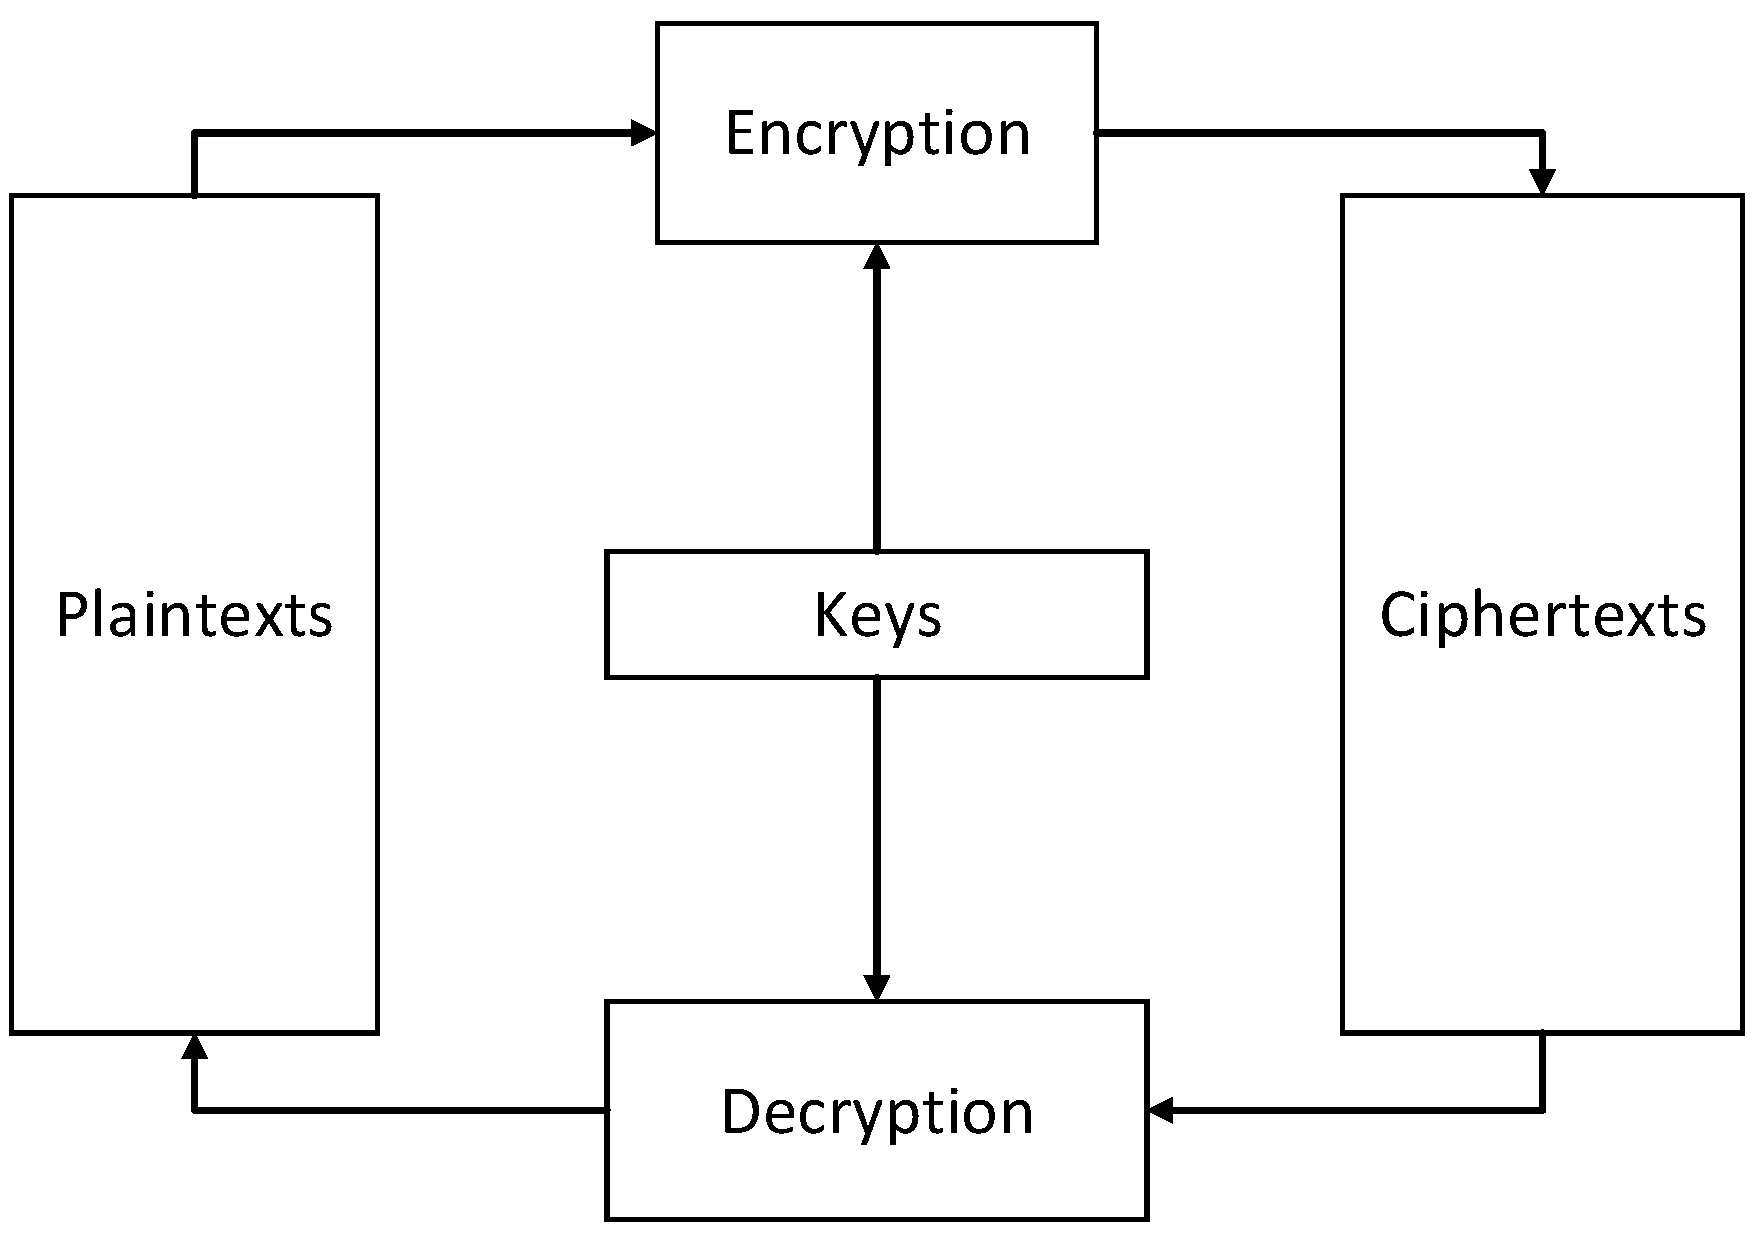
\includegraphics[width=0.7\textwidth , height = 5cm]{images/Cryptosystem}
    \caption{A basic cryptosystem}
    \label{fig:cryptosystem}
\end{figure}That means, a cryptosystem is a set of injective mappings from a finite set of plaintexts to a finite set of ciphertexts. Each key is associated with exactly one mapping. When the plaintext and the ciphertext space are equal the injective mappings are bijective. Figure \ref{fig:cryptosystem} shows a very high level picture of a cryptosystem. However, in this work, the terms \textit{cryptosystem} and \textit{cipher} have been used interchangeably. \par \noindent From the key management point of view, cryptosystems can be classified into two categories. One is public key cryptosystem and the other is symmetric key cryptosystem. In public key cryptosystem, the sender encrypts the message by the receiver\textquotesingle s public key before sending it. The encrypted message can only be decrypted by the receiver\textquotesingle s private key. The security of a public key cryptosystem depends on some computationally hard problems. Among many others, such difficult mathematical problems include discrete logarithm and integer factoring. RSA is a widely known, studied and used public key cryptosystem that uses the hardness of integer factoring as the basis of its security. In a symmetric key cryptosystem, both of the sender and the receiver share the same key which is secret from everyone else. This secret key is used to both encrypt and decrypt the message. Figures \ref{fig:symmetric_key_encryption} and \ref{fig:public_key_encryption} give a very high level view of a symmetric and public key cryptosystem. In both of the figures, Alice is the sender and Bob is the receiver. The security of such symmetric key cryptosystem primarily depends on its randomness, size of ciphertext space and key-length. Block ciphers and stream chiphers are examples of symmetric key cryptosystems. This thesis focuses on block ciphers.
\begin{figure}[h!]
    \centering
    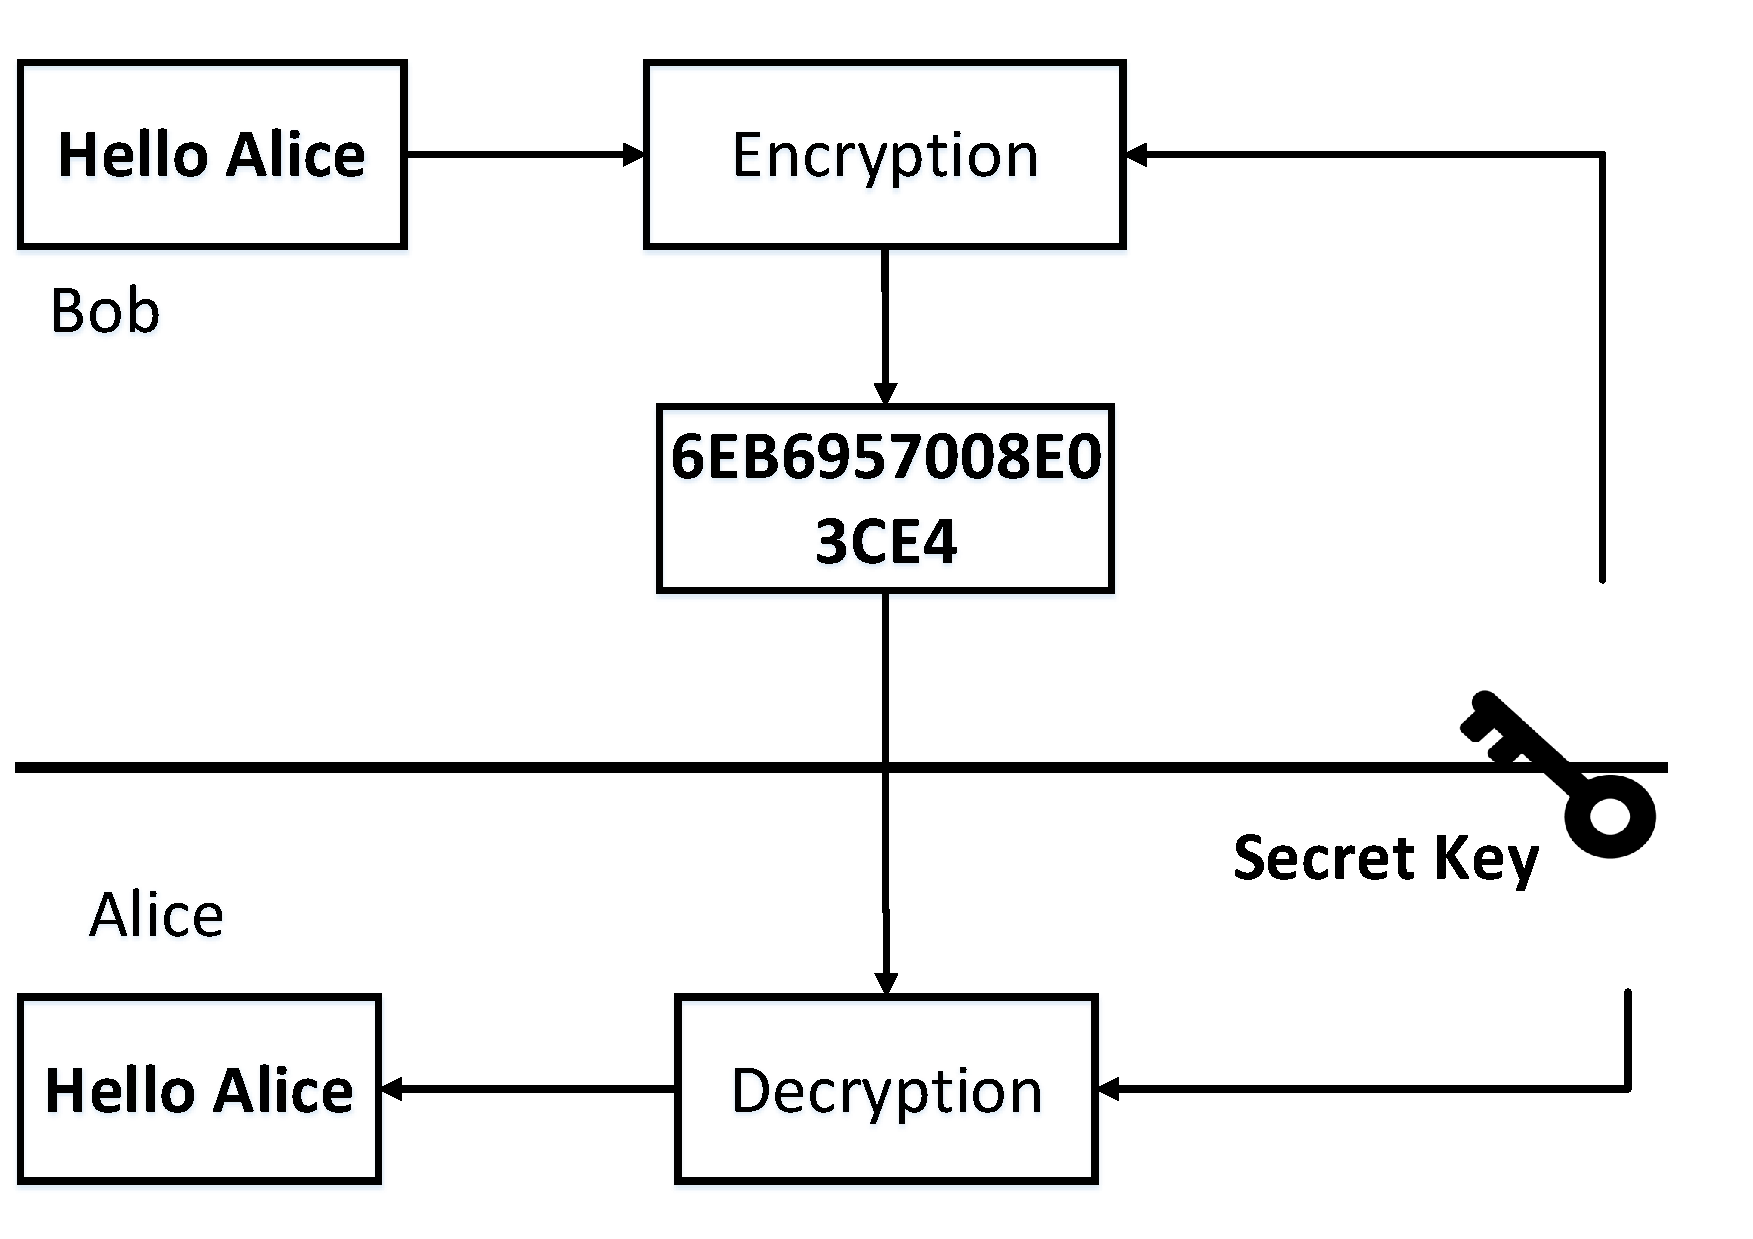
\includegraphics[width=.7\textwidth , height = 6cm]{images/SymmetricKeyEncryption}
    \caption{Symmetric key cryptosystem}
    \label{fig:symmetric_key_encryption}
\end{figure}
\begin{figure}[h!]
    \centering
    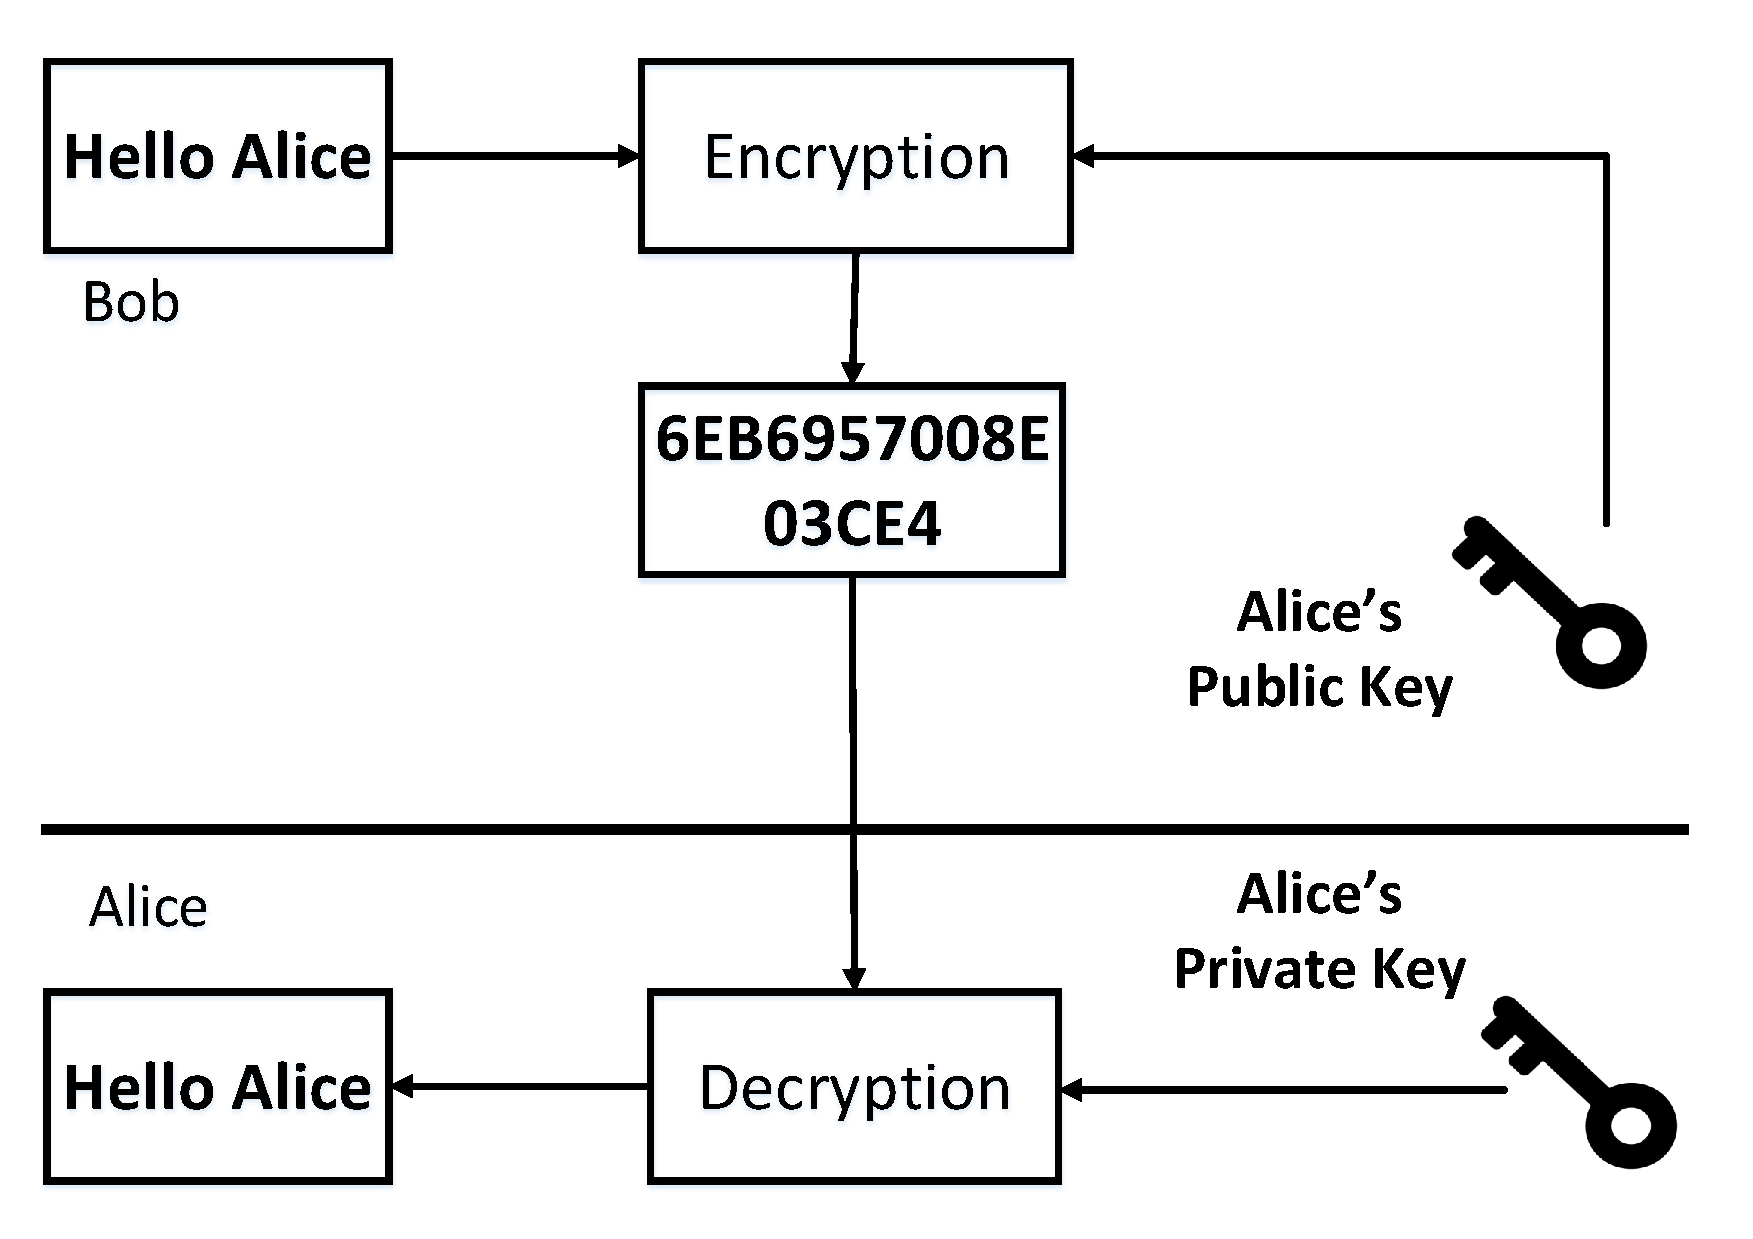
\includegraphics[width=.7\textwidth , height = 6cm]{images/PublicKeyEncryption}
    \caption{Public key cryptosystem}
    \label{fig:public_key_encryption}
\end{figure}
\section{Block Cipher} 
Block cipher is a symmetric key encryption system. The lowest level of granulairty of the encryption system is a block of bits. That is, the data to be encrypted is split into blocks $x_i$ of fixed length $n$ where $i \in \mathbb{N}$. A typical value of $n$ is $128$. And then it encrypts the whole block as a single plaintext and produce the ciphertext of the same length as the plaintext. Generally it can be written as 
\begin{eqnarray*}
\mathcal{P} &=& \mathcal{C} = \mathbb{Z}_2^n \\
\mathcal{K} &=& \mathbb{Z}_2^l
\end{eqnarray*}
For every $k \in \mathcal{K}$ there exists a bijective mapping $E_k:\mathcal{P} \rightarrow \mathcal{C}$. Generally, the mapping $E_k$ consists of repetitive applications of same set of operations. Each repetition is called a round. In each round the cipher often uses a different key which is called the round key. If a block cipher has $r$ number of rounds then there will be $r$ number of round keys denoted by $k^{1}, ...,k^{r}$ and the list of these keys, $(k^1,...,k^{r})$ is called the key schedule. The round keys are generated from a master key $k$ by a fixed key generation algorithm. This key generation algorithm is public. The first round of the cipher takes the plaintext as its input. The output of each round is considered as the input of the next round. The output of the final round is the ciphertext.
\begin{figure}[h!]
    \centering
    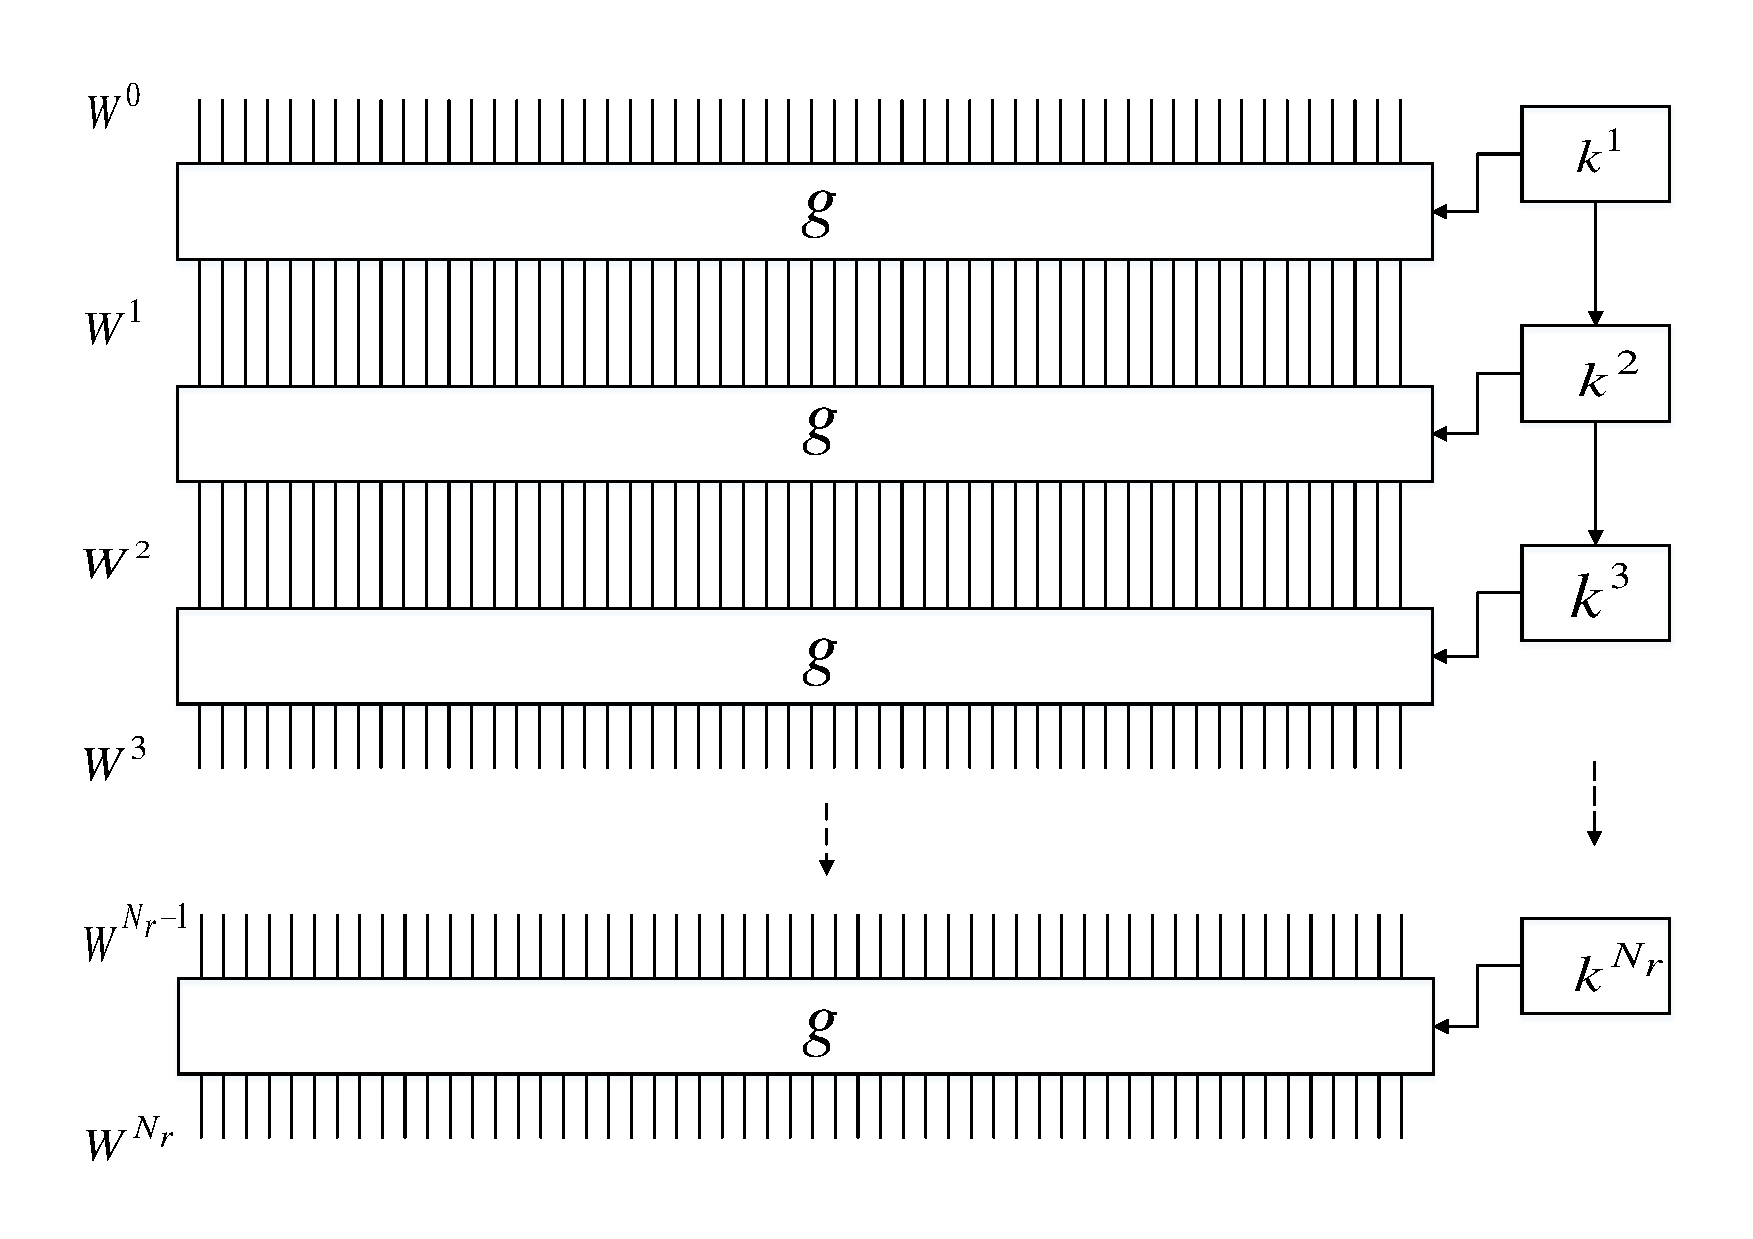
\includegraphics[width=.9\textwidth, height = 7cm]{images/BlockCipher}
    \caption{A block cipher}
    \label{fig:block_cipher}
\end{figure}If we denote the plaintext $x$ by $W^0$ and the ciphertext $E_k(x) = y$ by $W^{r}$ and the round function as $g:\mathcal{P \times \mathcal{K}} \rightarrow \mathcal{C}$, then the encryption of a block cipher can be computed by the Algorithm \ref{Algorithm_block_cipher_encryption}. Figure \ref{fig:block_cipher} shows the operation pictorially.
\begin{algorithm}
\caption{: $E(x,(k^1,...,k^{r}))$}
\label{Algorithm_block_cipher_encryption}
\begin{algorithmic}
\State $W^0 \leftarrow x$
\For {$i \leftarrow 1 \textbf{ to } r$}
	\State $W^{i} \leftarrow g(W^{i-1},k^{i})$
\EndFor
\State $\textbf{return }W^{r}$
\end{algorithmic}
\end{algorithm}
\par \noindent Decryption is applying the inverse of the function $g$ at every round. As we start from the ciphertext, we have to use the key in the reverse order. That is, we have to calculate $W^{r-1} = g^{-1}(W^{r},k^{r})$. Note that, $g$ has to be an injective mapping, otherwise $g^{-1}$ is not well defined. Using this process, we can decrypt the cipher by the Algorithm \ref{Algorithm_block_cipher_decryption}.
\begin{algorithm}
\caption{: $D(y,(k^1,...,k^{r}))$}
\label{Algorithm_block_cipher_decryption}
\begin{algorithmic}
\State $W^{r} \leftarrow y$
\For {$i \leftarrow r \textbf{ to } 1$}
	\State $W^{i-1} \leftarrow g^{-1}(W^{i},k^{i})$
\EndFor
\State $\textbf{return }W^{0}$
\end{algorithmic}
\end{algorithm}
However, based on the detail of function $g$ and the data structure used to hold the states, there are different kinds of block ciphers. The simplest one among those is SPN (Substitution-Permutation Network). In this thesis, SSA is experimented on an SPN named PRESENT. In the following section SPN is discussed in detail.

\subsection{Substitution-Permutation Networks }
\begin{defn} \label{SPN_definition} \citep{spn_definition_book}
Let $a,m$ and $r$ be positive integers, let $\pi_s:\left\lbrace 0,1 \right\rbrace^{a} \rightarrow \left\lbrace 0,1 \right\rbrace^{a}$ be a substitution, and let $\pi_p: \left\lbrace 1,...,am\right\rbrace \rightarrow \left\lbrace 1,...,am\right\rbrace$ be a permutation. Let $\mathcal{P} = \mathcal{C}=\left\lbrace 0,1 \right\rbrace^{am}$, and let $\mathcal{K} \subseteq (\left\lbrace 0,1 \right\rbrace^{am})^{r+1}$ consist of all possible key schedules that could be derived from an initial key $k$ using the key scheduling algorithm. For a key schedule $(k^1,...,k^{r+1})$, the encryption of plaintext is computed as Algorithm \ref{Algorithm_SPN}
\end{defn}
\begin{algorithm}
\caption{: $SPN(x,\pi_s,\pi_p,(k^1,...,k^{r+1}))$}
\label{Algorithm_SPN}
\begin{algorithmic}
\State $W^0 \leftarrow x$
\For {$r \leftarrow 1 \textbf{ to } r - 1$}
	\State $u^{r} \leftarrow W^{r-1} \oplus k^r$
	\For {$i \leftarrow 1 \textbf{ to m}$}
	\State $v^r_{<i>} \leftarrow \pi_s(u^r_{<i>})$
	\EndFor
	\State $W^r \leftarrow (v^r_{\pi_p(1)},...,v^r_{\pi_p(am)})$
\EndFor
\State $u^{r} \leftarrow W^{r-1} \oplus k^{r}$
\For {$i \leftarrow 1 \textbf{ to m}$}
\State $v^{r}_{<i>} \leftarrow \pi_s(u^{r}_{<i>})$
\EndFor
\State $y \leftarrow v^{r} \oplus k^{r+1}$
\State $\textbf{return }y$
\end{algorithmic}
\end{algorithm}Given an $am$ bit binary string, say $x = (x_1,...,x_{am})$, can be regarded as the concatenation of $m$ number of $a$-bit substrings, which can be denoted by $x_{<1>},...,x_{<m>}$. Thus
\begin{eqnarray*}
x &=& x_{<1>}||\cdots||x_{<m>}
\end{eqnarray*} 
and for $1 \leq i \leq m$, we have that 
\begin{eqnarray*}
x_{<i>} &=& (x_{(i-1)a+1},...,x_{ia})
\end{eqnarray*} The SPN consists of $r$ rounds. In each round (except for the last round, which is slightly different), we perform $m$ substitutions using $\pi_s$, followed by a permutation using $\pi_p$. Prior to each substitution operation, we incorporate the round key bits via a simple XOR operation, this is called round key mixing. In Algorithm \ref{Algorithm_SPN}, $u^r$ is the input to the $S$-boxes in round $r$, and $v^r$ is the output of the $S$-boxes after round $r$. $W^r$ is obtained from $v^r$ by applying the permutation $\pi_P$, and then $u^{r+1}$ is constructed from $W^r$ by XOR-ing with the round key $k^{r+1}$ . In the last round, the permutation $\pi_P$ is not applied. Now, we present an SPN as an example.
\begin{exmp}
\label{SPN_Example} \citep{spn_definition_book} Suppose that $a = m = r = 4$. Let $\pi_S$ and $\pi_P$ be defined by Table \ref{table: substitution_table} and \ref{table: permutation_table} respectively, where the input of $\pi_S$ are written in hexadecimal notation, $(0 \leftrightarrow (0,0,0,0), 1 \leftrightarrow (0,0,0,1),...,9 \leftrightarrow (1,0,0,1), A \leftrightarrow (1,0,1,0),...,F \leftrightarrow (1,1,1,1))$. 
\end{exmp}

\begin{table}
\centering
\begin{tabular}{|l|l|l|l|l|l|l|l|l|l|l|l|l|l|l|l|l|}
\hline
$z$ & $0$ & $1$ & $2$ & $3$ & $4$ & $5$  & $6$ & $7$ & $8$ & $9$ & $A$ & $B$ & $C$ & $D$  & $E$ & $F$ \\
\hline
$\pi_S(z)$ & $E$ & $4$ & $D$ & $1$ & $2$ & $F$ & $B$ & $8$ & $3$ & $A$ & $6$ & $C$ & $5$ & $9$ & $0$ & $7$  \\
\hline
\end{tabular}
\caption{Substitution function $\pi_S:\left\lbrace 0,1 \right\rbrace^{4} \rightarrow \left\lbrace 0,1 \right\rbrace^{4}$}
\label{table: substitution_table}
\end{table} 
\begin{table}
\centering
\begin{tabular}{|l|l|l|l|l|l|l|l|l|l|l|l|l|l|l|l|l|}
\hline
$z$ & $0$ & $1$ & $2$ & $3$ & $4$ & $5$  & $6$ & $7$ & $8$ & $9$ & $10$ & $11$ & $12$ & $13$  & $14$ & $15$ \\
\hline
$\pi_P(z)$ & $1$ & $5$ & $9$ & $13$ & $2$ & $6$ & $10$ & $14$ & $3$ & $7$ & $11$ & $15$ & $4$ & $8$ & $12$ & $16$  \\
\hline
\end{tabular}
\caption{Permuation function:$\pi_P: \left\lbrace 0,1,...,15\right\rbrace \rightarrow \left\lbrace 0,1,...,15\right\rbrace$}
\label{table: permutation_table}
\end{table}
\begin{figure}[h!]
    \centering
    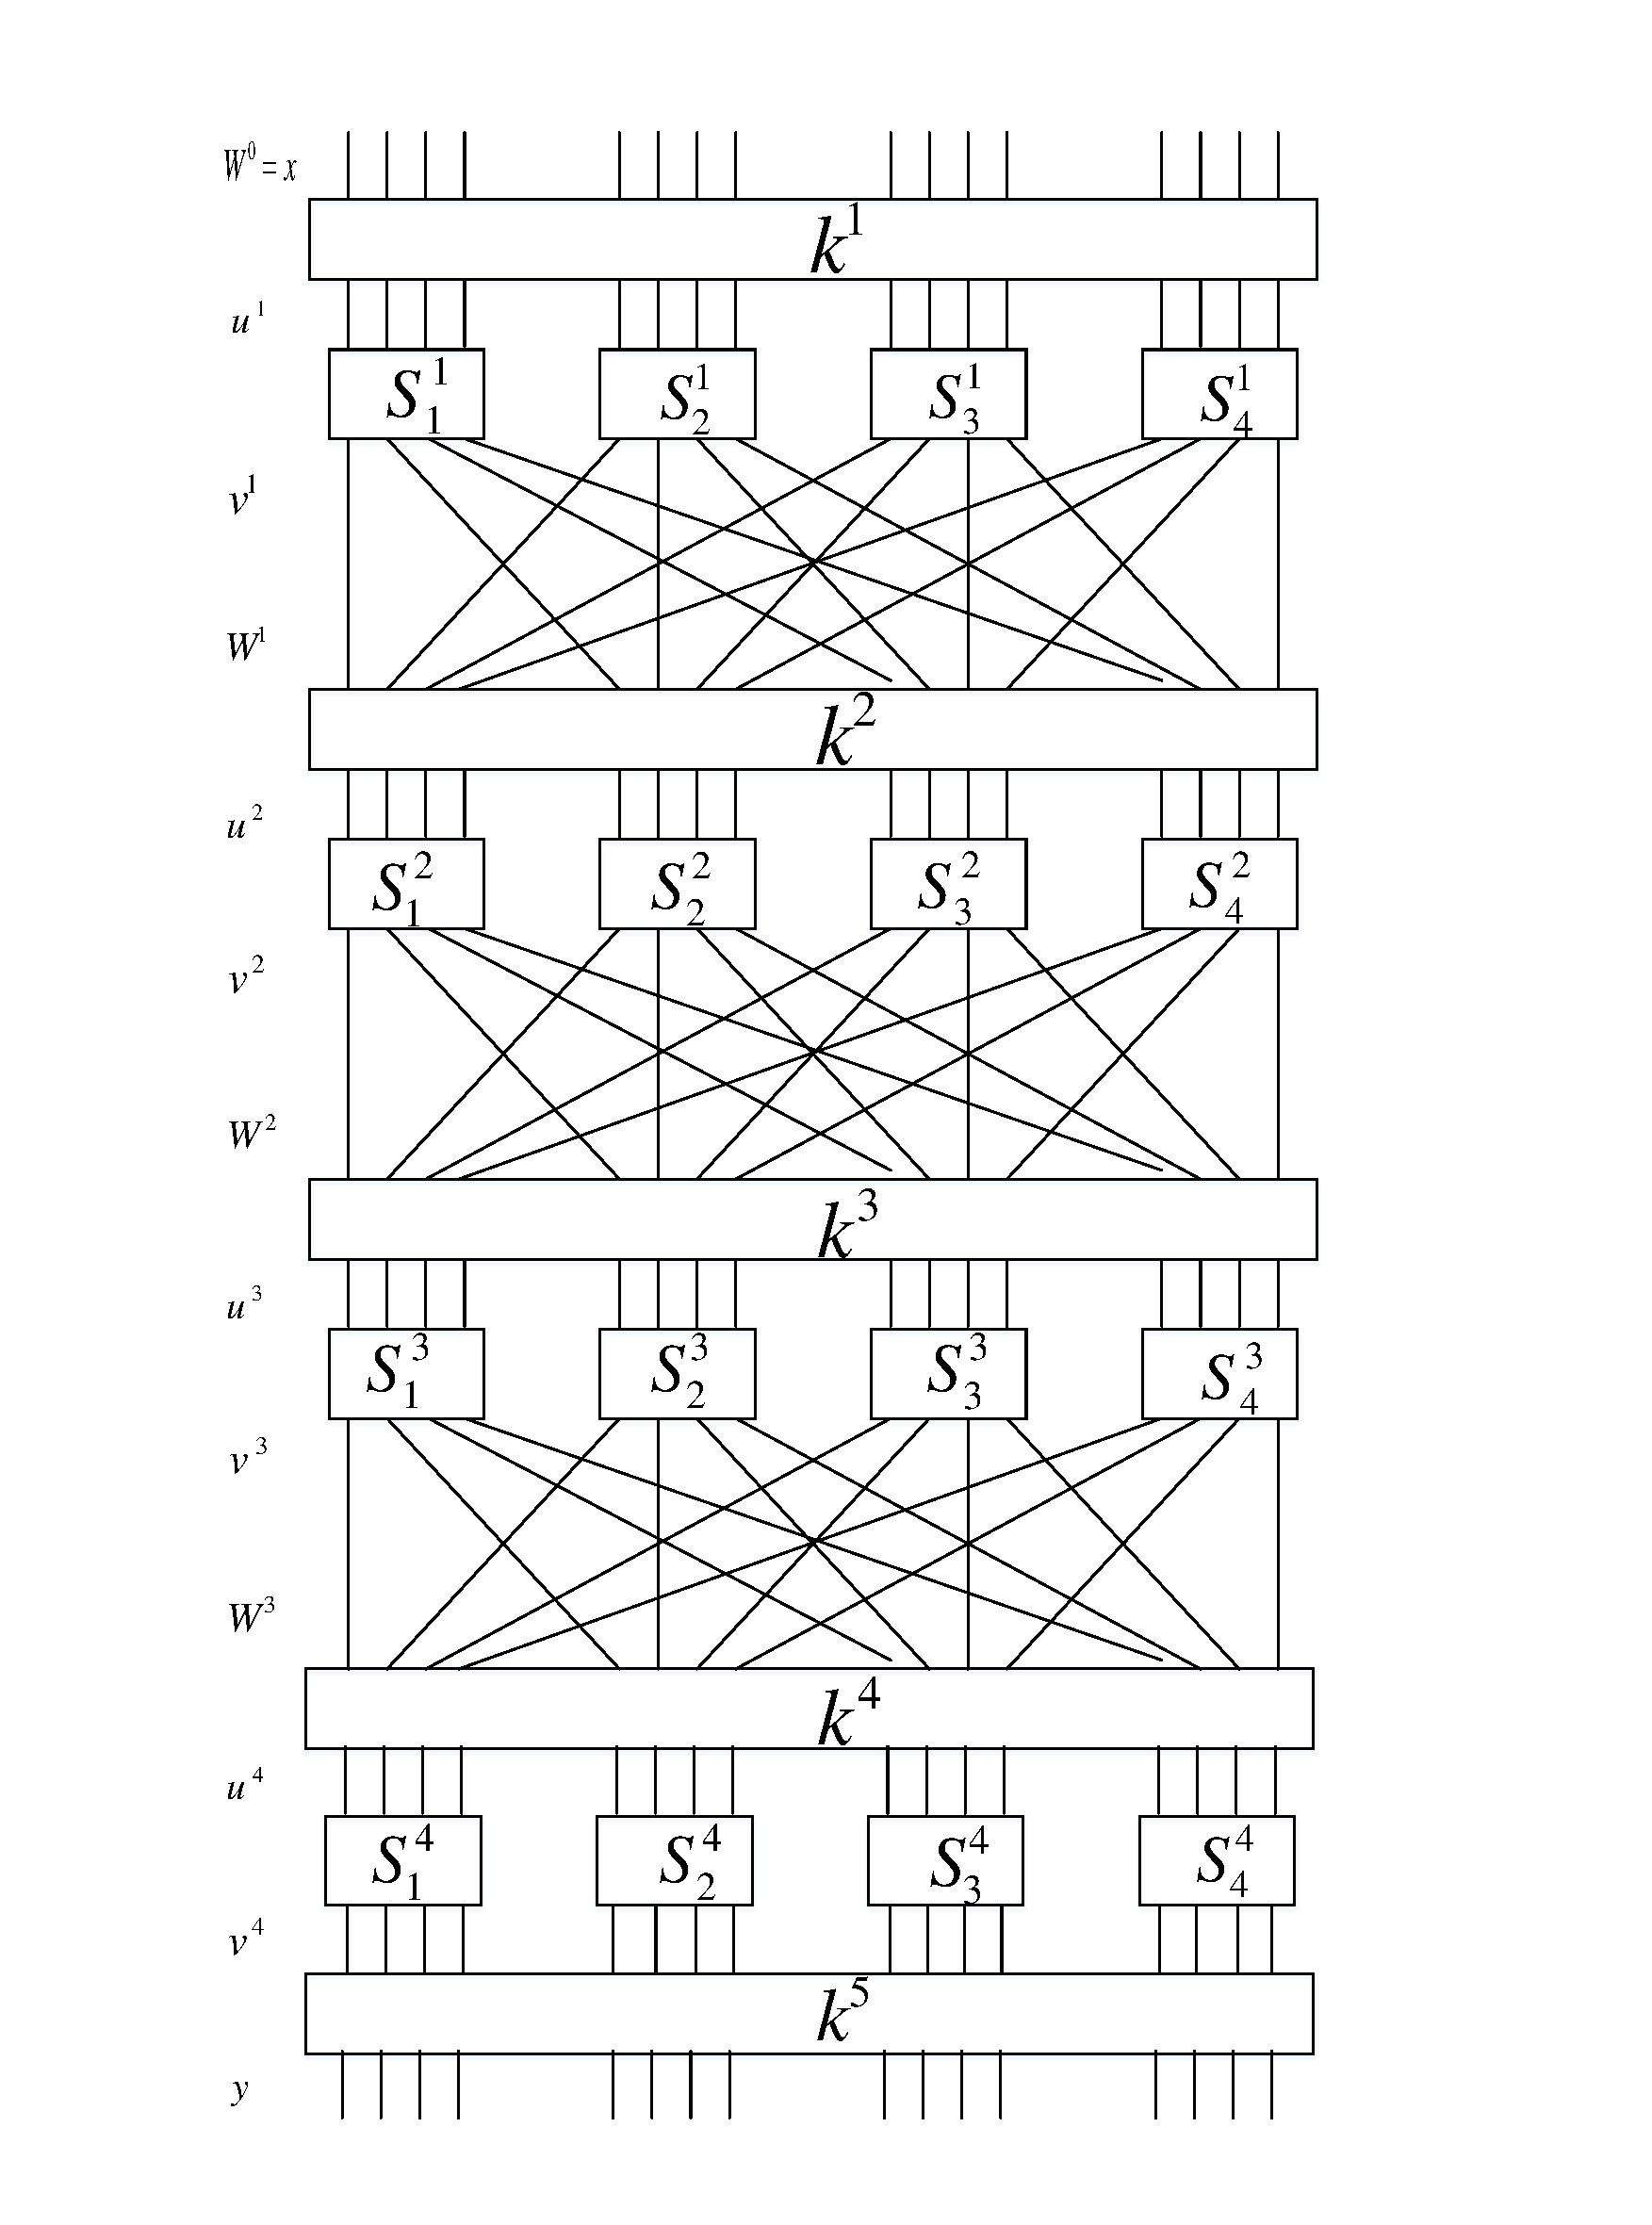
\includegraphics[width=.9\textwidth, height=16cm]{images/SPNDiagram}
    \caption{A substitution-permutation network}
    \label{fig:SPN}
\end{figure}See Figure \ref{fig:SPN} for a pictorial representation of this particular SPN. In this diagram, we have named the $S$-boxes $S_{i}^r$ $(1 \leq i,r \leq 4)$. All $16$ S-boxes incorporate the same substitution function based on $\pi_S$.\par \noindent
In order to complete the description of the SPN, we need to specify a key scheduling algorithm. Here is a simple possibility: suppose that we begin with a $32$-bit key $k = (k_1,...,k_{32}) \in \left\lbrace 0,1 \right\rbrace^{32}$. For $1 \leq r \leq 5$, define $k^r$ to consist of $16$ consecutive bits of $k$, beginning with $k_{4r-3}$. This may not be a very secure way to define a key schedule; we have just chosen something easy for purposes of illustration.\par \noindent SPNs have simple and very efficient design, in both hardware and software. The SPN in Example \ref{SPN_Example} is not secure, if for no other reason that the key length ($32$ bits) is small enough that an exhaustive key search is feasible. However, ``larger" SPNs can be designed that are secure against all known attacks. In this work, we use SPN as the test bed of the statistical model of SSA. As of now, we have defined cryptosystems, block ciphers and SPN. In Section \ref{section:cryptanalysis} we have discussed the general philosophy of statistical cryptnalysis of a block cipher and the state of the art in this field of research. Then we define the SSA formally. In Chapter \ref{chapter:statistical_distinguishers}, we start to derive our statistical model.
\section{Cryptanalysis} \label{section:cryptanalysis}
National Security Agency (NSA) has defined cryptanalysis as the analytic investigation of an information system with the goal of illuminating hidden aspects of that system. It encompasses any systematic analysis aimed at discovering features in, understanding aspects of, or recovering hidden parameters from an information system \cite{def_cryptanalysis}.\par \noindent This thesis work considers the information system to be a block cipher and the systematic analysis exploits the statistical properties of the cipher in question. The process we have followed is broadly known as statistical cryptanalysis. The process includes finding a statistic (preferably parametrized) computable from the cipher system which significantly deviates from the value of the same statistic computed in a uniformly random set up. The process also includes the task of finding the parameter that causes the statistic to deviate the most from random. As the statistic and the parameter is chosen, the cryptanalysis uses a large set of ciphertexts or plaintext-ciphertext pairs associated with the cipher in attack to compute the statistic. Comparing the value of this computed statistic with some known statistic can reveal other hidden information of the cipher. Depending on the statistic used and the way it is exploited, there are many different kinds of statistical cryptanalysis. Some of the very well known statistical cryptanalytic techniques include linear, ML, differential, TD, integral, and SS cryptanalysis. \par \noindent In linear attacks, the statistic used is the correlation of a linear approximation. The linear approximation is obtained by applying a mask on the inputs and a mask on the outputs of the cipher. The correlation of the linear approximation is calculated by comparing how many times the function outputs $1$ and how many times it outputs $0$. Using this statistic, a cipher can be distinguished from random and the last round key can also be partially recovered. Over the years, cryptanalysts have found tricky ways to define this linear approximation. In ML attack, the linear approximation has multiple input and output masks. Based on their correlations, the theoretical distribution of partial plaintext-ciphertext pairs is computed. The input and output masks are chosen in a way so that the distribution deviates by large values from the uniform distribution. \par \noindent On the other hand, in differential attacks, a different statistic is used. It considers the probability of a differential. That is, it checks the probability of pairs of plaintexts with some fixed difference to have certain fixed difference in their corresponding ciphertexts. If a differential is identified for a cipher which has a significantly different probability than in the random case, then that differential can be used to reveal other hidden information of the cipher. In general, the metric used to calculate the difference among the plaintext pairs and ciphertext pairs is bitwise $XOR$. Like linear cryptanalysis, differential cryptanalysis also has its variants. One such variant is truncated differential cryptanalysis. In TD attacks, the differential probability considers only certain bits of plaintexts and ciphertexts while ignoring the other bits. \par \noindent In SSA, the statistic of the distribution of ciphertext or plaintext-ciphertext is considered. Certain bits of the plaintexts are kept fixed while the other bits can vary. SSA encrypts a large number of such plaintexts and exploits the distribution of certain bits of the corresponding ciphertexts. In Section \ref{section:present}, SSA is formally explained  and in Chapter \ref{chapter:statistical_distinguishers}, the derivation of the statistical model of SSA is presented in detail. However, as Collard and Standaert applied this attack on the block cipher PRESENT, we also have selected PRESENT and its small versions \citep{smalpresent} as the test bed of SSA. As a result, before discussing SSA in  detail, it will be useful to discuss the specification of present PRESENT in brief.


\section{PRESENT} \label{section:present}
PRESENT is a Substitution-Permutation Network with a block size of $64$ bits designed by Bogdanov et al. \cite{bogdanov_PRESENT} in $2007$. The recommended key size is $80$ bits, which should be sufficient for the expected applications of the cipher. However, a 128-bit key-schedule is also proposed. The encryption is composed of $31$ rounds. Each of the $31$ rounds consists of a non-linear substitution layer, a linear bitwise permutation layer and a bitwise XOR operation with round key $K_i$ where $1 \leq i \leq 32$. Note that, $K_{32}$ is used for postwhitening. The non-linear layer uses a single $4$-bit S-box which is applied $16$ times in parallel in each round. 
\begin{figure}[h!]
    \centering
    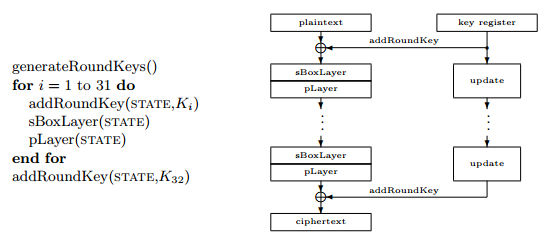
\includegraphics[width=0.9\textwidth]{images/presentCipherAlgorithm}
    \caption{Top-level algorithmic description of PRESENT \cite{SSA_Collard_Standaert}.}
    \label{fig:PRESENT_block_diagram}
\end{figure}  The linear permutation is defined by Table  \ref{table:permutation_table_PRESENT} where bit $i$ of input is moved to bit position $P(i)$. The $4$-bit S-box is defined according to Table 
\ref{table:substitution_table_PRESENT}. We do not mention the key-schedule here as we do not make explicit use of it in our distinguishing attack. Figure $\ref{fig:present_spn}$ shows the substitution-permutation network pictorially for one round.\begin{figure}[h!]
    \centering
    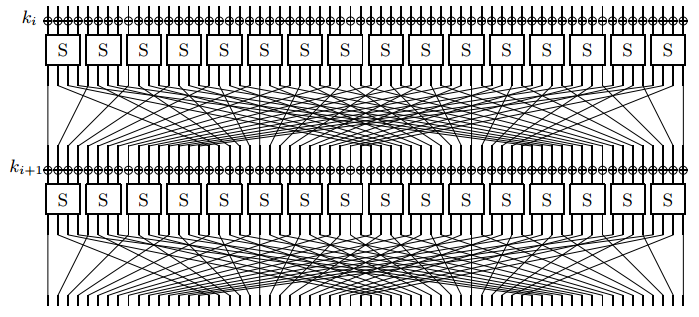
\includegraphics[width=0.9\textwidth]{images/presentCipherSPNetwork}
    \caption{PRESENT SPN \cite{SSA_Collard_Standaert}.}
    \label{fig:present_spn}
\end{figure}
\begin{table}
\centering
\begin{scriptsize}
\begin{tabular}{|l|l|l|l|l|l|l|l|l|l|l|l|l|l|l|l|l|}
\hline
$i$ & $0$ & $1$ & $2$ & $3$ & $4$ & $5$  & $6$ & $7$ & $8$ & $9$ & $10$ & $11$ & $12$ & $13$  & $14$ & $15$ \\
\hline
$p(i)$ & $0$ & $16$ & $32$ & $48$ & $1$ & $17$ & $33$ & $49$ & $2$ & $18$ & $34$ & $50$ & $3$ & $19$ & $35$ & $51$  \\
\hline
\hline
$i$ & $16$ & $17$ & $18$ & $19$ & $20$ & $21$  & $22$ & $23$ & $24$ & $25$ & $26$ & $27$ & $28$ & $29$  & $30$ & $31$ \\
\hline
$p(i)$ & $4$ & $20$ & $36$ & $52$ & $5$ & $21$ & $37$ & $53$ & $6$ & $22$ & $38$ & $54$ & $7$ & $23$ & $39$ & $55$  \\
\hline
\hline
$i$ & $32$ & $33$ & $34$ & $35$ & $36$ & $37$ & $38$ & $39$ & $40$ & $41$ & $42$ & $43$ & $44$ & $45$ & $46$ & $47$ \\
\hline
$p(i)$ & $8$ & $24$ & $40$ & $56$ & $9$ & $25$ & $41$ & $57$ & $10$ & $26$ & $42$ & $58$ & $11$ & $27$ & $43$ & $59$  \\
\hline
\hline
$i$ & $48$ & $49$ & $50$ & $51$ & $52$ & $53$ & $54$ & $55$ & $56$ & $57$ & $58$ & $59$ & $60$ & $61$ & $62$ & $63$ \\
\hline
$p(i)$ & $12$ & $28$ & $44$ & $60$ & $13$ & $29$ & $45$ & $61$ & $14$ & $30$ & $46$ & $62$ & $15$ & $31$ & $37$ & $63$  \\
\hline
\end{tabular}
\end{scriptsize}
\caption{Permutation layer of PRESENT}
\label{table:permutation_table_PRESENT}
\end{table}

\begin{table}
\centering
\begin{scriptsize}
\begin{tabular}{|l|l|l|l|l|l|l|l|l|l|l|l|l|l|l|l|l|}
\hline
$i$ & $0$ & $1$ & $2$ & $3$ & $4$ & $5$  & $6$ & $7$ & $8$ & $9$ & $A$ & $B$ & $C$ & $D$  & $E$ & $F$ \\
\hline
$S[i]$ & $C$ & $5$ & $6$ & $B$ & $9$ & $0$ & $A$ & $D$ & $3$ & $E$ & $F$ & $8$ & $4$ & $7$ & $1$ & $2$  \\
\hline
\end{tabular}
\end{scriptsize}
\caption{S-box of PRESENT (hexadecimal notation).}
\label{table:substitution_table_PRESENT}
\end{table} 


\section{Non-linearity of the S-box in PRESENT}
It is important for any block cipher to be non-linear to be immune against different kind of cryptanalytic attacks \citep{Celine_Kaisa_non_linear_functions,Kaisa_perfect_non_linear_functions}. PRESENT is not an exception. The S-box in PRESENT is a non-linear function. However, being non-linear is not a guarantee for the expected security. Cryptanalysts try to find out linear approximations of the non-linear function with sufficiently deviated correlation which eventually opens up a weakness of the cipher. A good S-box is the one which minimizes deviation of the correlations from zero for all the possible linear approximations. Correlation is a measure of the non-uniformity of a binary function. Let $f:\mathbb{F}_2^n \rightarrow \mathbb{F}_2$ is a boolean function. Then the correlation of function $f$ denoted by $\mathbf{cor}_x\left(f\right)$ is defined in \citep{Celine_Kaisa_Links_2013} as its correlation with the all-zero function as following 
\begin{eqnarray}
\mathbf{cor}_x\left(f\right) &=& \frac{1}{2^n}\left[\# \left\lbrace x \in \mathbb{F}_2^n \;|\;f\left(x\right) = 0 \right\rbrace - \# \left\lbrace x \in \mathbb{F}_2^n \;|\;f\left(x\right) \neq 0 \right\rbrace \right]
\end{eqnarray}
A linear approximation $f:\mathbb{F}_2^n \rightarrow \mathbb{F}_2$ of a vectorial boolean function $\mathbf{F}:\mathbb{F}_2^n \rightarrow \mathbb{F}_2^n$ is developed by considering an input and an output mask $\alpha,\beta \in \mathbb{F}_2^n$ in the following way
\begin{eqnarray}
f_{\left(\alpha,\beta \right)} \left( x \right) &=& \alpha \cdot x \oplus \beta \cdot \mathbf{F}\left( x \right)
\end{eqnarray} where the notation ``$\cdot$'' represents standard inner product.
The S-box used in PRESENT is a vectorial boolean function $S:\mathbb{F}_2^4 \rightarrow \mathbb{F}_2^4$ mentioned in Table \ref{table: substitution_table}. So, given an input mask $\alpha \in \mathbb{F}_2^4$ and an output mask $\beta \in \mathbb{F}_2^4$, and a vectorial boolean function $S$, the correlation of the linear approximation $f_{\left(\alpha,\beta \right)} = \alpha \cdot x \oplus \beta \cdot S\left(x\right)$ is measured as follows:
\begin{eqnarray*}
\mathbf{cor}_x\left(f_{\left(\alpha,\beta \right)}\right) &=& \frac{1}{2^n}\left[\# \left\lbrace x \in \mathbb{F}_2^n \;|\; f_{\left(\alpha,\beta \right)}\left(x\right) = 0 \right\rbrace - \# \left\lbrace x \in \mathbb{F}_2^n\;|\;f_{\left(\alpha,\beta \right)}\left(x\right) \neq 0 \right\rbrace \right]
\end{eqnarray*}
The correlation table of the S-box of PRESENT is given in Table \ref{table:correlation_matrix} \citep{j_y_cho_linear_cryptanalysis}. We have discussed how this table helps in preparing an SSA in Section \ref{section:choosing_ssa_trail}. In Chapter \ref{chapter:experiment}, we have shown in detail how this table helps in finding a feasible SSA attack on SMALLPESENT-$[n]$.
\begin{table}
\centering
\begin{tiny}
\begin{tabular}{|l|l|l|l|l|l|l|l|l|l|l|l|l|l|l|l|}
\hline
$\alpha / \beta$&$1$&$2$&$3$&$4$&$5$&$6$&$7$&$8$&$9$&$A$&$B$&$C$&$D$&$E$&$F$ \\
\hline
$1$&$0$&$\frac{1}{4}$&$0$&$0$&$-\frac{1}{2}$&$0$&$-\frac{1}{2}$&$0$&$0$&$0$&$0$&$0$&$-\frac{1}{2}$&$0$&$\frac{1}{2}$  \\ \hline
$2$&$0$&$\frac{1}{4}$&$\frac{1}{4}$&$-\frac{1}{4}$&$-\frac{1}{4}$&$0$&$0$&$\frac{1}{4}$&$-\frac{1}{4}$&$0$&$\frac{1}{2}$&$0$&$\frac{1}{2}$&$-\frac{1}{4}$&$\frac{1}{4}$  \\ \hline
$3$&$0$&$\frac{1}{4}$&$\frac{1}{4}$&$\frac{1}{4}$&$-\frac{1}{4}$&$-\frac{1}{2}$&$0$&$-\frac{1}{4}$&$\frac{1}{4}$&$-\frac{1}{2}$&$0$&$0$&$0$&$-\frac{1}{4}$&$-\frac{1}{4}$  \\ \hline;
$4$&$0$&$-\frac{1}{4}$&$\frac{1}{4}$&$-\frac{1}{4}$&$-\frac{1}{4}$&$0$&$\frac{1}{2}$&$-\frac{1}{4}$&$-\frac{1}{4}$&$0$&$-\frac{1}{2}$&$0$&$0$&$-\frac{1}{4}$&$\frac{1}{4}$  \\ \hline
$5$&$0$&$-\frac{1}{4}$&$\frac{1}{4}$&$-\frac{1}{4}$&$\frac{1}{4}$&$0$&$0$&$\frac{1}{4}$&$\frac{1}{4}$&$-\frac{1}{2}$&$0$&$\frac{1}{2}$&$0$&$\frac{1}{4}$&$\frac{1}{4}$  \\ \hline
$6$&$0$&$0$&$-\frac{1}{4}$&$0$&$0$&$-\frac{1}{2}$&$0$&$0$&$-\frac{1}{2}$&$0$&$0$&$\frac{1}{2}$&$0$&$0$&$0$  \\ \hline
$7$&$0$&$0$&$\frac{1}{4}$&$\frac{1}{2}$&$0$&$0$&$0$&$0$&$-\frac{1}{2}$&$0$&$0$&$0$&$0$&$\frac{1}{2}$&$0$  \\ \hline
$8$&$0$&$\frac{1}{4}$&$-\frac{1}{4}$&$0$&$0$&$-\frac{1}{4}$&$\frac{1}{4}$&$-\frac{1}{4}$&$\frac{1}{4}$&$0$&$0$&$-\frac{1}{4}$&$\frac{1}{4}$&$\frac{1}{2}$&$\frac{1}{2}$  \\ \hline
$9$&$\frac{1}{2}$&$-\frac{1}{4}$&$-\frac{1}{4}$&$0$&$0$&$\frac{1}{4}$&$-\frac{1}{4}$&$-\frac{1}{4}$&$-\frac{1}{4}$&$-\frac{1}{2}$&$0$&$-\frac{1}{4}$&$\frac{1}{4}$&$0$& $0$  \\ \hline
$A$&$0$&$\frac{1}{2}$&$0$&$\frac{1}{4}$&$\frac{1}{4}$&$0$&$-\frac{1}{4}$&$\frac{1}{4}$&$0$&$0$&$-\frac{1}{2}$&$\frac{1}{4}$&$\frac{1}{4}$&$-\frac{1}{4}$&$\frac{1}{4}$  \\ \hline
$B$&$-\frac{1}{2}$&$0$&$0$&$-\frac{1}{4}$&$-\frac{1}{4}$&$\frac{1}{4}$&$-\frac{1}{4}$&$-\frac{1}{4}$&$0$&$0$&$0$&$\frac{1}{4}$&$\frac{1}{4}$&$\frac{1}{4}$& $-\frac{1}{4}$  \\ \hline
$C$&$0$&$0$&$0$&$-\frac{1}{4}$&$-\frac{1}{4}$&$-\frac{1}{4}$&$-\frac{1}{4}$&$\frac{1}{4}$&$0$&$0$&$-\frac{1}{2}$&$-\frac{1}{4}$&$\frac{1}{4}$&$\frac{1}{4}$&$-\frac{1}{4}$  \\ \hline
$D$&$\frac{1}{2}$&$\frac{1}{2}$&$0$&$-\frac{1}{4}$&$-\frac{1}{4}$&$\frac{1}{4}$&$\frac{1}{4}$&$0$&$0$&$0$&$0$&$\frac{1}{4}$&$-\frac{1}{4}$&$\frac{1}{4}$&$-\frac{1}{4}$  \\ \hline
$E$&$0$&$\frac{1}{4}$&$\frac{1}{4}$&$-\frac{1}{2}$&$\frac{1}{2}$&$-\frac{1}{4}$&$-\frac{1}{4}$&$-\frac{1}{4}$&$-\frac{1}{4}$&$0$&$0$&$-\frac{1}{4}$&$-\frac{1}{4}$&$0$&$0$\\ \hline
$F$&$\frac{1}{4}$&$\frac{1}{4}$&$\frac{1}{4}$&$0$&$0$&$-\frac{1}{4}$&$-\frac{1}{4}$&$-\frac{1}{4}$&$\frac{1}{4}$&$-\frac{1}{2}$&$0$&$\frac{1}{4}$&$\frac{1}{4}$&$0$&$0$  \\ \hline
\end{tabular}
\end{tiny}
\caption{Correlation table of S-box of PRESENT: $\mathbf{cor}_x\left(f_{\left( \alpha, \beta \right)} \right)$}
\label{table:correlation_matrix}
\end{table} 


\section{SSA} \label{section:SSA}
SSA is a chosen plaintext attack. It means the attacker has access to an encryption oracle and can encrypt any plaintext without knowing the encryption key. As the idea of SSA has already been mentioned in the introduction, we will now define it formally and discuss the basic principle of finding a weakness in a block cipher to mount an SSA. \par \noindent Let the length of the input and the output block of the SPN is $n$. Then the set of plaintexts and ciphertexts can be considered as a set of vectors of length $n$ defined over the field $\mathbb{F}_2$, that is $\mathbb{F}_2^n$. Let $x^i$ denote the $i$-th element of the vector $x \in \mathbb{F}_2^n$.  As the assumed weakness of the cipher suggests, we find four integers $s,t,q$ $r$ such that $s+t = q+r = n$ and $B_s, B_t, B_q, B_r \subseteq [n]$ are subsets of all the possible bit positions. $|B_s| = s, |B_t|=t, |B_q| = q,|B_r|=r$ and $B_s \cap B_t = B_q \cap B_r = \emptyset$ and $|B_s \cup B_t| = |B_q \cup B_r| = \emptyset$. \par \noindent That is, the bit positions are partitioned into two disjoint parts in possibly two different ways. Then the plaintexts are chosen in a way so that the bits in positions $B_s$ are kept fixed while the bits in positions $B_t$ vary. In this fashion, sufficiently large number of plaintexts are chosen and encrypted. Then from all the ciphertext achieved from this process is observed by focusing only on the bits in $B_q$. The distribution of the bits in $B_q$ is supposed to be non-uniform enough to be used in a statistical test given that the plaintext and chiphertext space partition has been done based on a weakness. In this scenario, the sets $B_s$ and $B_q$ form what is called an SS trail. We call $B_s$ as the input and $B_q$ as the output of the trail.
\section{Constructing an SS trail for PRESENT} \label{section:choosing_ssa_trail}
The strenght of an SSA depends on the non-uniformity of the the distribution at the output of the trail associated with the attack. In an SPN, in every round, apart from the key mixing, there are two layers. One is the non-linear layer which is called the sBoxLayer and the other is the linear layer called pLayer. The target is to choose certain bits from the plaintext space of the cipher so that they are strongly correlated with certain other bits in the ciphertext space across the sBoxLayer and pLayer of all the rounds under consideration. Then those strongly correlated bits in the plaintext and ciphertext space will form a useful SS trail. \par \noindent One way to find such correlations is to select a set of input and output bits (from the round function of the SPN) for the trail in such a way that the output bits of every round will after the permutation be the input bits of the next round. \par \noindent Now if we encrypt many plaintexts by ensuring extreme non-uniformity in those input bits at the very first round (in other words, fixing those input bits in the plaintext  space), then because of the bijective property of the S-box, there will be some degree of non-uniformity in the output bits of the selected S-box. In addition, because of the correlation among the selected input and output bits of the S-box, there will also be a certain level of non-uniformity in the chosen output bits of the first round. As the selection of the bits is made in a way that the selected output bits of the round function is permuted only among the input bit positions, the distribution of the input bits of the  next round will also remain non-uniform. In this fashion, after $r$ number of rounds, the output bits will remain non-uniform to certain degree. And thus the chosen input and output bits define the trail. However, the non-uniformity decreases as the number of rounds increases. So, naturally a good SS trail is the one which provides useful non-uniformity in the chosen output bits even after a significantly large value of $r$. \par \noindent An S-box is a bijective function from a set of binary vectors to a set of binary vectors. As this is a bijection, applying non-uniformity in the inputs of an S-box will also produce non-uniformity in its output. Let the non-uniformity of the inputs of an S-box is generated by making only one specific input bit non-uniform. Let this specific input bit is $x_i$. Then such non-uniformity in the input will generate non-uniformity in those output bits $y_j$ which has non-zero correlation with $x_i$. If for $i \neq j$, two input bits $x_i,x_j$ has non-zero correlation with output bit $y_k$, then the non-uniformity of $y_k$ achieved by the non-uniformity of both of the bits $x_i$ and $x_j$ is higher than the non-uniformity achieved by the non-uniformity of only one of $x_i$ or $x_j$. \par \noindent This suggests that, the input and output bits of the trail should be chosen in such a way that the number of input bits are maximized in one S-box. However, this also forces the number of output bits to be maximized in one S-box because the chosen output bits of one round become the chosen input bits of the next round. Note that if a chosen input bit $x_i$ of an S-box has zero correlation with a chosen output bit $y_j$ of the same S-box, then applying non-uniformity on $x_i$ doesn't produce any non-uniformity on $y_j$. This suggests to avoid choosing any pair of input-output bits from the same S-box which have zero correlation accross that S-box.

\subsection{SS trails in PRESENT}
Let us visualize the S-box in PRESENT as shown in Figure \ref{fig:S-box}. The leftmost input bit $x_0$ is considered as the least significant bit. By observing Table \ref{table:correlation_matrix}, we find that input bit $x_0$ has zero correlation with all the output bits $y_i$ where $0\leq i \leq 3$. We also find that input bit $x_3$ has zero correlation with output bit $y_2$. The 1 bit trails in case of zero correlations are marked using the red lines. As a result a good SS trail should include the bits from every S-box in a way that $x_0$ is not included at all and $x_3,y_2$ are not present in the trail simultaneously.
\begin{figure}[h!]
    \centering
    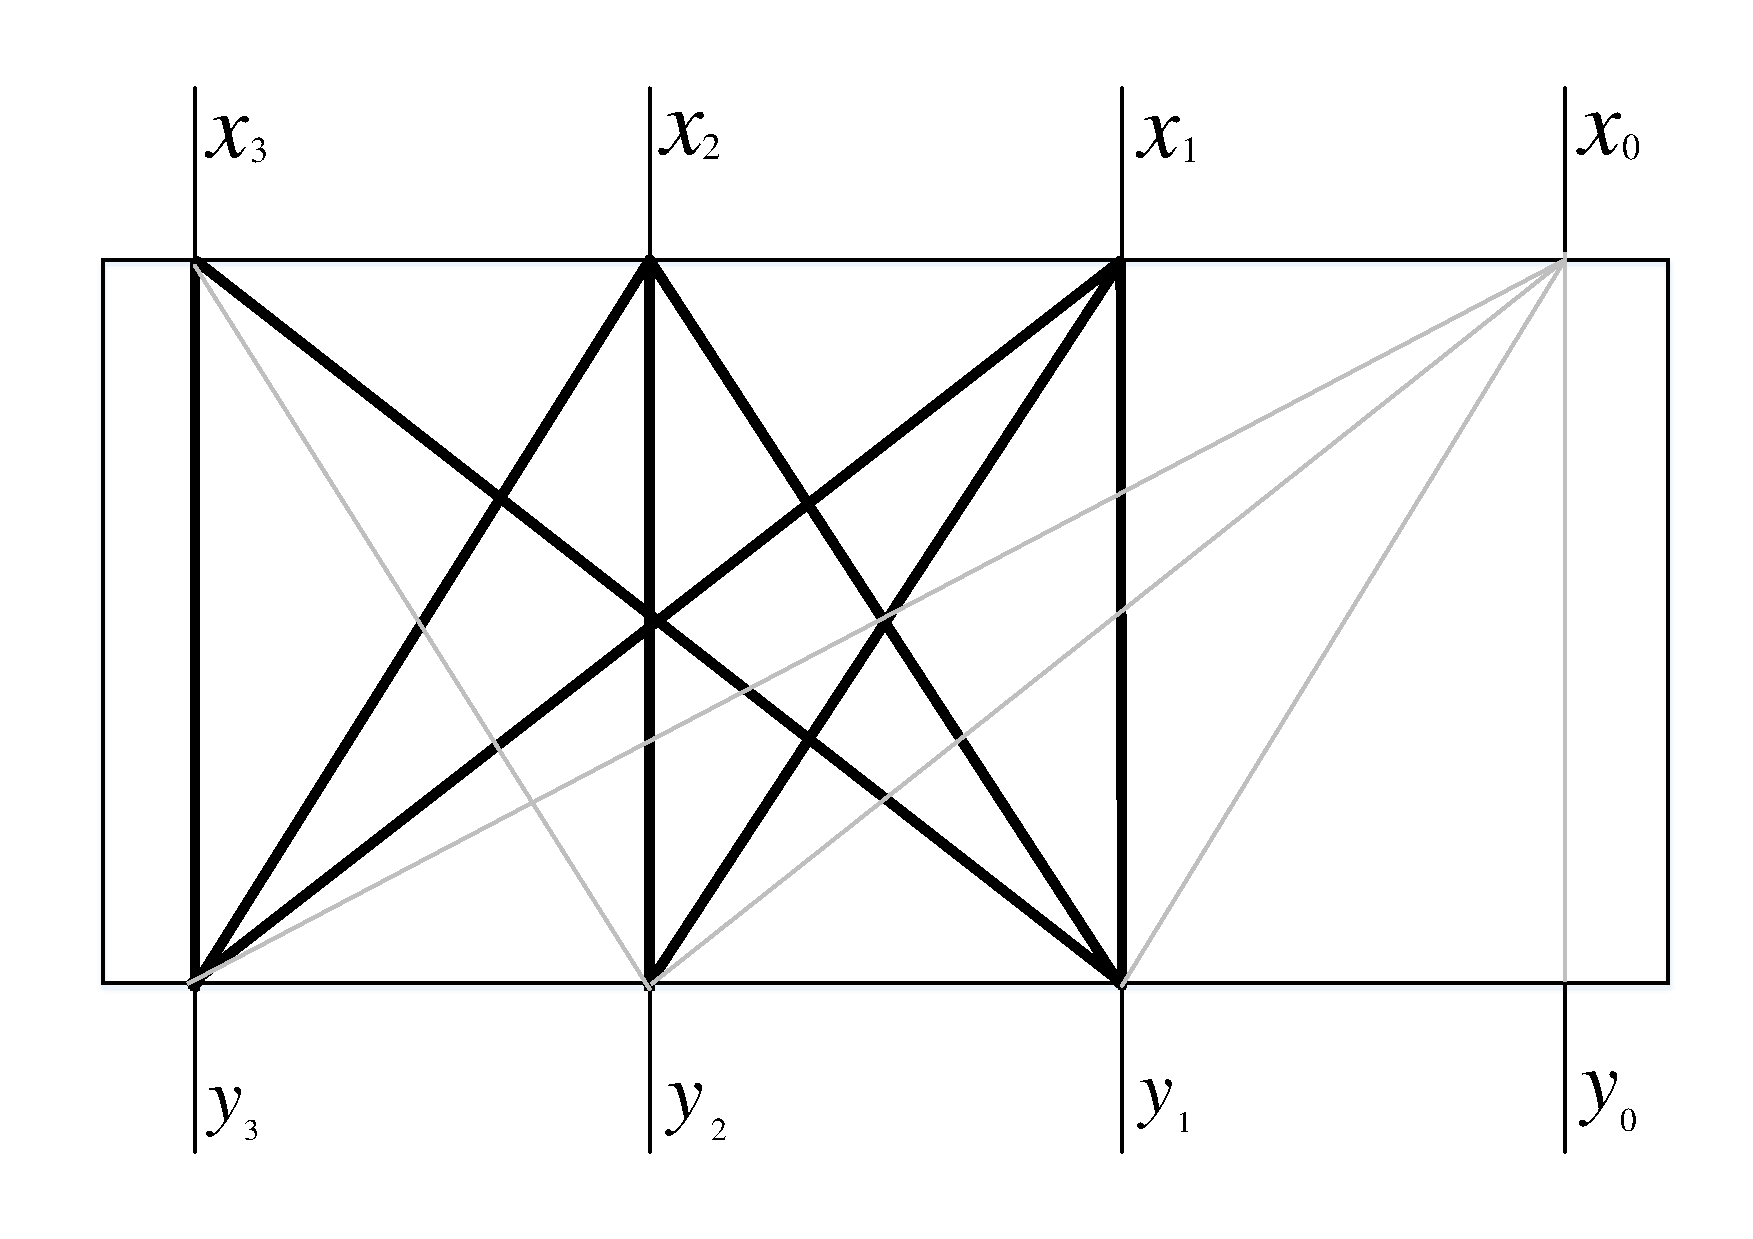
\includegraphics[width=0.9\textwidth,height = 6cm]{images/S-box_PRESENT}
    \caption{1 bit trails in the S-box of PRESENT.}
    \label{fig:S-box}
\end{figure}


\begin{figure}[h!]
    \centering
    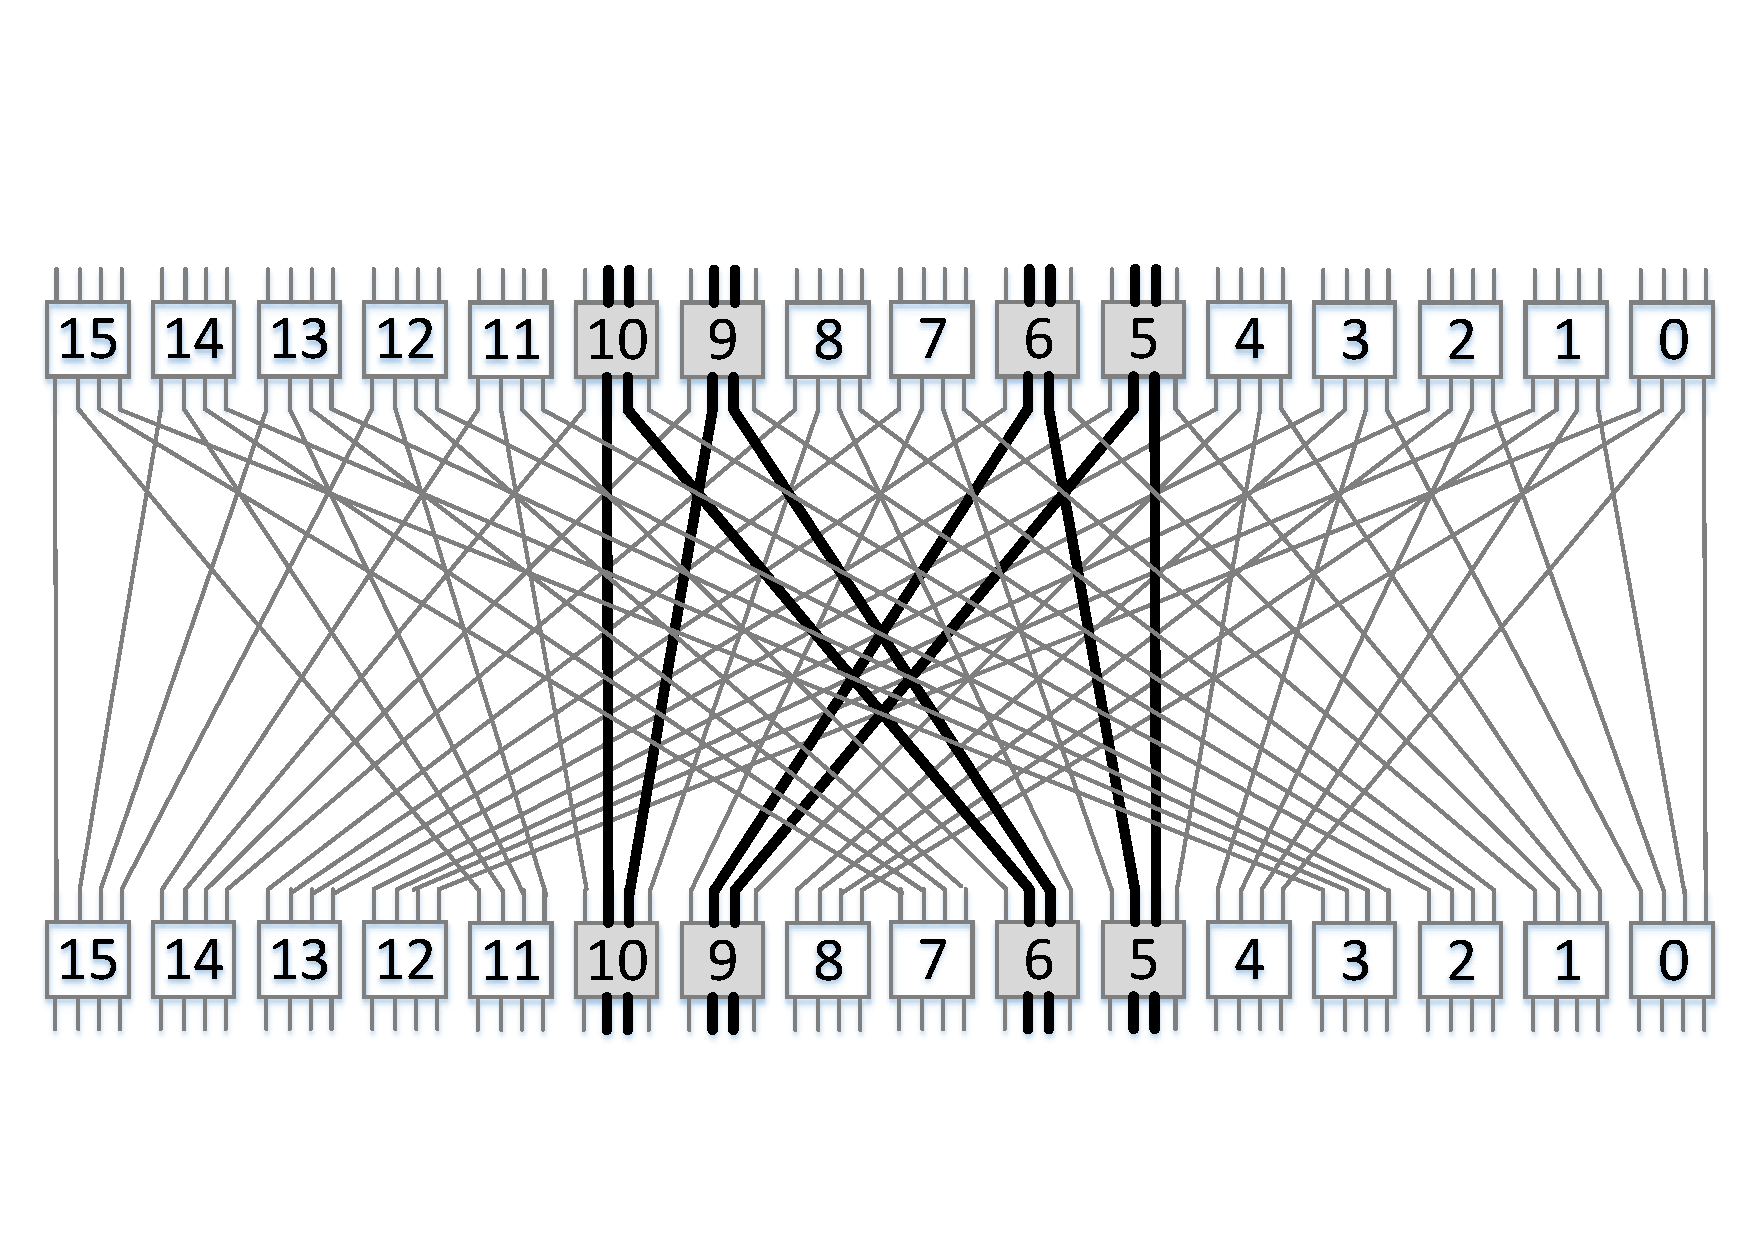
\includegraphics[width=0.9\textwidth]{images/presentCipherPoorDiffusionweakness}
    \caption{Weakness in PRESENT \cite{SSA_Collard_Standaert}.}
    \label{fig:present_weakness}
\end{figure}
There is a weakness in the permutation layer of PRESENT as described in Figure \ref{fig:present_weakness} \cite{SSA_Collard_Standaert}. The size of a block is $n=64$. Counting the plaintext bits starting from $0$ from the right, the $21,22,25,26,37,38,41,42$ bits are active only in $4$ S-boxes. And none of these bits are $x_0,x_3$ or $y_2$. So, it is expected that if we fix these $8$ bits (extreme non-uniformity) for each plaintext that we encrypt, then after encrypting sufficiently large amount of plaintexts, the ciphertexts will also have non-uniformity in the same $8$ bits. That is, the evolution of these $8$ bits are not random enough. As a result, we have a partitioning of the plaintext and ciphertext space. In the partitioning $s = q = 8$, $t = r = 56$, $B_s = B_q = \left\lbrace 21,22,25,26,37,38,41,42 \right\rbrace$ and $B_t = B_r = \left\lbrace 0,1,...,63  \right\rbrace \setminus B_s$.
\par \noindent Another interesting SS trail is mentioned in Figure \ref{fig:27bittrailPRESENT}. This trail has $27$ bits at its input and $27$ bits at its output. There are $9$ active S-boxes. Every S-box has $3$ input and $3$ output bits. That means in every S-box there are $3 \times 3 = 9$ different $1$ bit to $1$ bit trail. Note that this SS trail includes $x_3,y_2$ simultaneously which is unlike the principle we discussed in previous section. The reason, it is still a good SS trail is, out of the $9$ trails in every S-box, $x_3,y_2$ bits are involved in only one of them simultaneously. This results into $8$ active trails in every S-box whereas by excluding both of them we could have at most $2 \times 2 = 4$ active trails in every S-box. That means, even though $x_3,y_2$ has zero correlation among them across the S-box, it is still useful to include them in a trail as they contribute in generating other active trails.
\begin{figure}[h!]
    \centering
    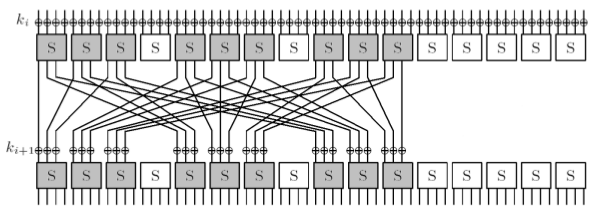
\includegraphics[width=0.9\textwidth]{images/27bittrailPRESENT}
    \caption{Weakness in PRESENT \cite{SSA_Collard_Standaert}.}
    \label{fig:27bittrailPRESENT}
\end{figure}

\section{Exploiting the Weakness}
In \cite{SSA_Collard_Standaert}, the authors proposed two techniques to exploit the weakness. In both of the techniques a sufficient number of chosen plaintexts are encrypted where $x_s$ part of $x$ is fixed to a value $a$.

\subsection{Comparing with Model Distribution} In order to exploit this weakness, the model distribution of $y_q$ part of $y$ is evaluated by Algorithm \ref{alg:theoretical_distribution} for each key guess. For one key guess at each round, the work needed to compute the model distribution of the target trail after $r$ round is equivalent to $r \cdot 2^{16}$ partial encryptions. Once the model distributions are computed, the key of the model distribution that minimizes the distance with the distribution computed from a secret key is accepted to be the correct key. 
\begin{algorithm}
\caption{: Computing model distribution}
\label{alg:theoretical_distribution}
\begin{algorithmic}[1]
\State Input: $8$-bit subkey guess $sk$ and the $8$-bit input distribution $distrib\_in[256]$
\State Output: the $8$-bit output distribution $distrib\_out[256]$\\
\State initialize $distrib\_out[256]$ to the all-zero state
\For {$8$-bit values $text$}
	\For {$8$-bit values $rand$}
		\State fix the $8$-bit trail to $text$ and xor with $sk$
		\State fix the $8$-bit non-trail to $rand$
		\State apply the S-boxes
		\State apply the permutation
		\State evaluate the value of the $8$ bit trail out
		\State update $distrib\_out[out]= distrib\_out[out] + distrib\_in[text]/256$;
	\EndFor
\EndFor
\end{algorithmic}
\end{algorithm}
\par \noindent To verify the practicability of the attack model, Collard and Standaert have conducted an experiment on reduced-round version of PRESENT. To reduce the number of key guess, they have simplified the key scheduling algorithm by using the same key in each round. They have used $2^{30}$ chosen plaintexts. In all those plaintexts, the $8$ bits (mentioned in Figure \ref{fig:present_weakness} in bold lines) are fixed, and the other $56$ bits are varied. All those plaintexts are encrypted where round keys are kept fixed in each round. Then they have computed the distribution of those fixed $8$ bits at the end of $2,4,6$ and $8$ round. These experimental distributions computed from the real cipher itself with reduced-round and modified key scheduling algorithm is compared with the model distributions computed from Algorithm \ref{alg:theoretical_distribution} for $2,4,6$ and $8$ rounds. According to this simplified experiment, both experimental and model distributions present a significant deviation from uniform as expected. \par \noindent They also have made an observation on the distance in between the experimental and model distributions. First they have computed the experimental and model distributions of the concerned $8$ bits at the end of $2,4,6$ and $8$ rounds for the key byte $32$ (i.e. $00100000$). Then they have computed the model distributions of these $8$ bits for all possible $256$ sub-keys at the end of $2,4,6$ and $8$ rounds. Finally they have plotted the distance in between the model distribution for every possible key bytes and model disribution of key byte $32$. For the sake of discussion, let us call this distance to be model-model distance. They also have plotted the distance in between the model distribution for every possible key bytes and experimental disribution of key byte $32$. Let us call this distance to be model-experiment distance. It has been found that the distance between the model-model and model-experiment distance is minimized at the correct key. This indicates that the model distribution captures the essence of the experimental distribution. \par \noindent In both of the experiments it has been found that the deviation tends to decrease with number of rounds. So, as the number of rounds increases, to find significant deviation, the number of chosen plaintext is also needed to be increased. In other words, as the number of rounds increases, the data complexity of the attack also increases.
\par \noindent However, in the attack mentioned above, the effect of the key scheduling algorithm has been ignored to show that the basic idea works in principle. Now considering the key scheduling algorithm, demands more key bits to be guessed as the round key changes in every round. As for one round we need to guess at most $8$ bits, we are in need of guessing at most $r \times 8$ bits after $r$ rounds. According to Collard and Standaert, for $12$ rounds of PRESENT, $63$ key bits have to be guessed, meaning, there are $2^{63}$ different possible keys in effect. For each key guess, after $r$ rounds, we are in need of computing $r \times 2^{16}$ partial encryptions. Which implies that we are in need of $2^{63} \times r \times 2^{16}$ partial encryptions. We see that the attack becomes quite impossible even with $12$ rounds because of its time complexity. In the next section, we present a tricky way to overcome this problem. The idea is the same as in commonly used statistical linear and differential attacks. Instead of guessing key bits on the intermediate rounds, make a prediction about the behaviour of the cipher over those rounds that holds on the average over the keys.

\subsection{Distinguishing Attack:} Computing the theoretical distribution is costly. To overcome this problem, they suggest a distinguishing attack which we will explain in brief here. The plaintexts are encrypted using $r$-rounds of PRESENT and record the distribution of the ciphertexts for the $16$ bits at the output of the $4$ active $S$-box in the last round. Given this experimental distribution, it is possible to compute the output distribution of the target $8$-bit trail one round before by a classical partial decryption process. For one key guess, the evaluation of such $r-1$-round distribution requires $2^{16}$ computations. For the corect key guess, the experimental $8$-bit distribution in the $r-1$-round is expected to be more non-uniform than for any other guess. This is because decrypting with a wrong guess is expected to have the same effect as encrypting one more round. Thus it is expected to distinguish the correct key from the wrong ones by computing the distance between a partially decrypted distribution and the uniform distribution. If the attack works properly, the distribution with the highest distance should correspond to the correct key. \par \noindent There are extensions of this distinguishing attack. The same attack can be made by increasing the number of fixed plaintext bits or by using multiple fixations of the fixed bits or by doing partial decryption for $2$ rounds instead of $1$ round. However, all these extensions require to distinguish a distribution from uniform distribution. The statistical model developed in this work is a statistic $T$ which can be used to perform a statistical test that can distinguish the computed distribution in between two known distributions. In the next sections, we have defined formally the notion of a distribution. We will also recall some known distributions and their properties as they will be useful in finding the statistical model. In the next chapter we have presented how to perform a statistical test to distinguish a distribution between two given distributions. In the next chapter we have defined the statistic $T$ and used it to develop a SS distinguisher in Chapter \ref{chapter:statistical_distinguishers}. In Chapter \ref{chapter:data_complexity_of_SSA}, we have shown how the success probability of the statistical test is related with the number of plaintexts we encrypt before performing the statistical test.

\chapter{Statistics}
\label{chapter:statistics} 
\section{Probability Distribution}
Probability distribution is a function from a set of possible outcomes of an experiment to a set of real values in the range $[0,1]$. The sum of the probabilities of occurrences of all the possible outcomes is always $1$. Now if the set of possible outcomes contains only discrete values then the function that defines the probability distribution is called probability mass function (pmf). If the set of possible outcomes contains continuous value within any range, then the function that defines the probability distribution of the experiment is called probability density function (pdf). \par \noindent There are different kinds of probability density and probability mass functions that describes the probability distribution of many natural events. Few of these probability distributions have been found to be very important in developing the statistical model of SSA. In this section those distributions along with their properties are discussed briefly
\subsection{Gamma Distribution} 
\begin{defn} \citep{gamma_distribution_book} A random variable X that is gamma-distributed with shape $k$ and scale $\theta$ is denoted by
\begin{eqnarray*}
X \sim \Gamma(k, \theta) \equiv \textrm{Gamma}(k, \theta)
\end{eqnarray*}
The probability density function using the shape-scale parametrization is
\begin{eqnarray*}
f(x;k,\theta) =  \frac{x^{k - 1}e^{-\frac{x}{\theta}}}{\theta^k\Gamma(k)} \quad \mbox{ for } x > 0 \mbox{ and } k, \theta > 0
\end{eqnarray*}
Here $\Gamma(k)$ is the gamma function evaluated at $k$.
\end{defn}
Figure \ref{fig:gamma_dist}  provides a visualization of the gamma distribution given different shape and scale parameters.
\begin{figure}[h!]
    \centering
    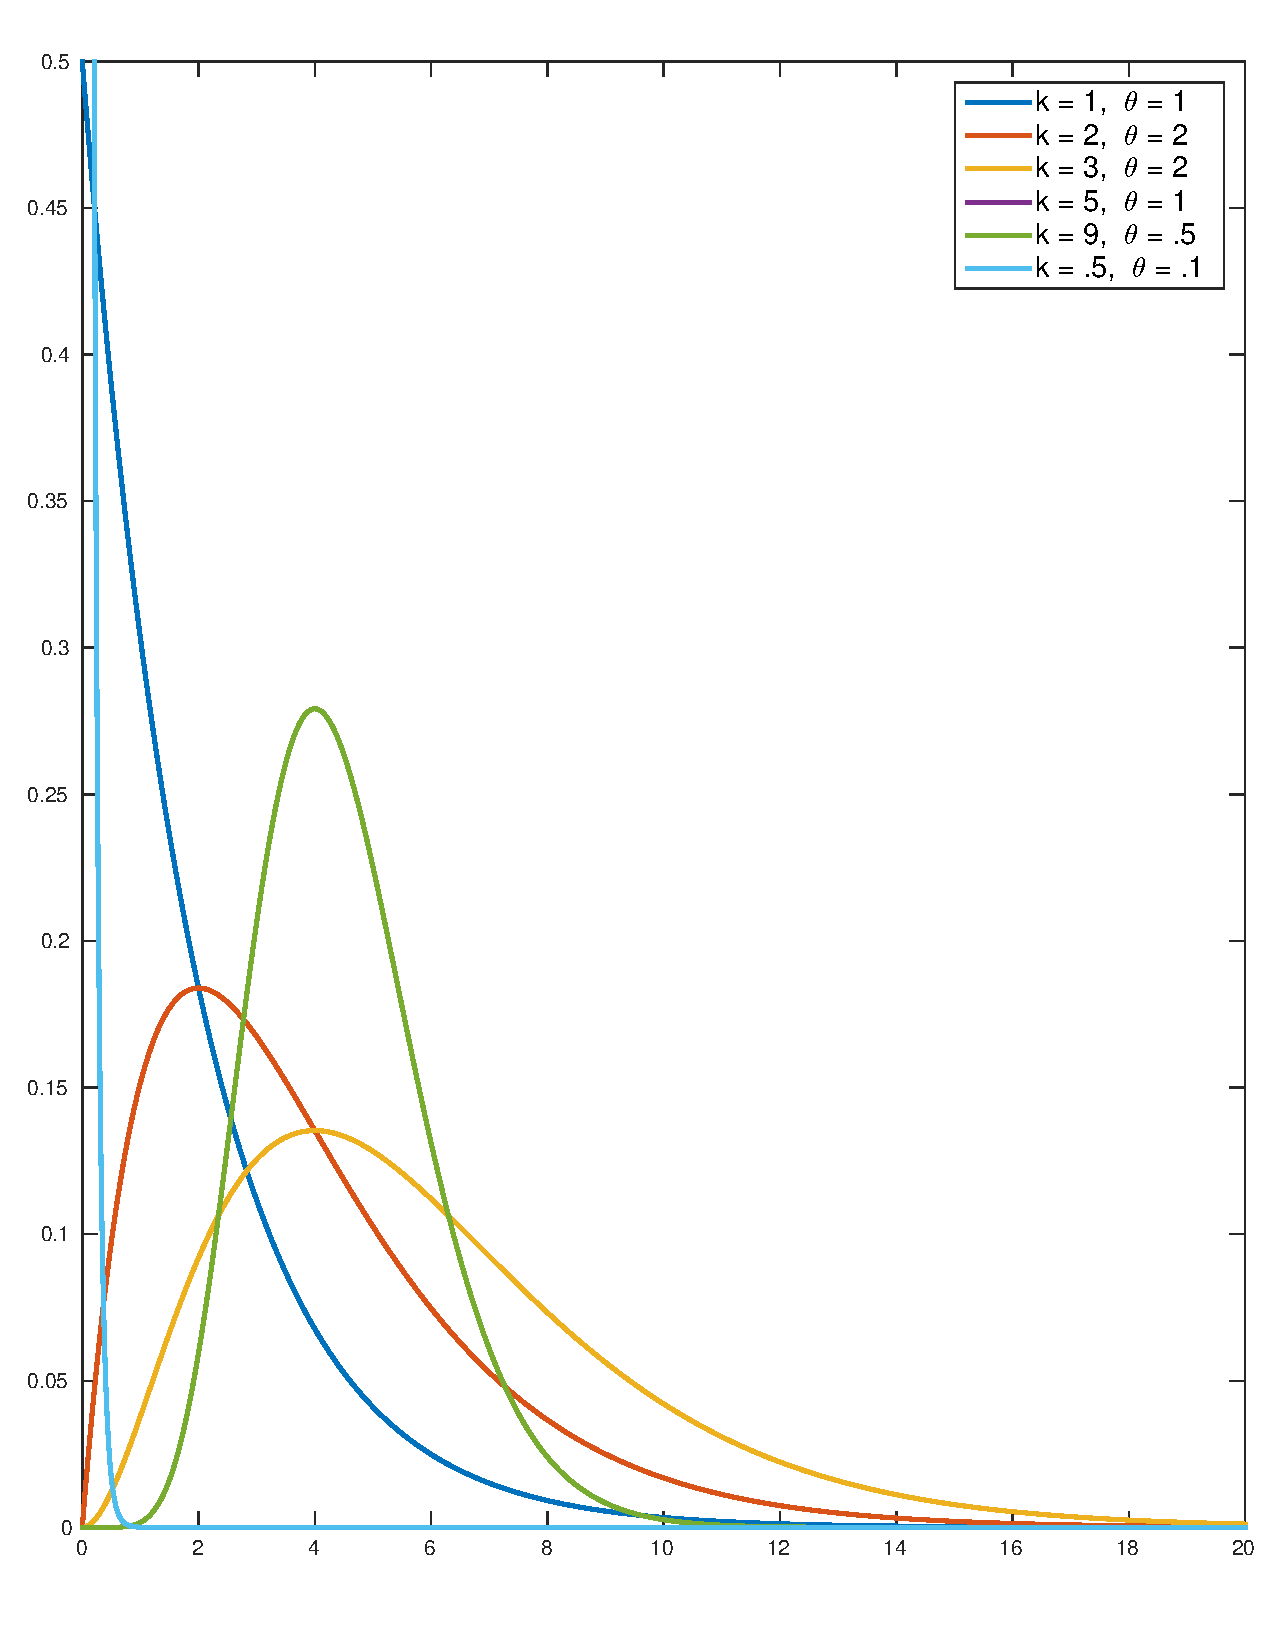
\includegraphics[width=0.9\textwidth, height=12cm]{images/GammaDistribution}
    \caption{Gamma distribution with different shape and scale parameters}
    \label{fig:gamma_dist}
\end{figure}
\subsection{Properties of Gamma Distribution}
\begin{enumerate}
\item Let $X$ be a random variable which is gamma distributed with shape parameter $k$ and scale parameter $\theta$. Then for any constant $c$, the random variable $Y = cX$ is also gamma distributed with the shape parameter $k^{'}$ and scale parameter $\theta^{'}$. Where $k^{'} = k$ and $\theta^{'} = c\theta$ \cite{scaling_of_gamma_distribution_uah}. In other words, we can write
\begin{eqnarray}
X \sim \Gamma(k,\theta) \Rightarrow cX \sim \Gamma(k,c\theta)\label{eqn:gamma_dist_property_scaling}
\end{eqnarray}
\item Le $X$ be a random variable which is gamma distributed with the shape parameter $k$ and scale parameter $\theta$. Then the mean and variance of $X$ denoted by $\mu_X$ and $\sigma^2_X$ respectively are defined as follows \citep{gamma_distribution_book}
\begin{eqnarray}
\mu_X &=& k \theta  \label{eqn:mean_gamma_dist} \\
\sigma^2_X &=& k \theta^2 \label{eqn:variance_gamma_dist}
\end{eqnarray}

\end{enumerate}
\subsection{$\chi^2$-Distribution} \citep{chi_square_definition_book} In probability theory and statistics, the chi-squared distribution (also chi-square or $\chi^2$-distribution) with $k$ degrees of freedom is the distribution of a sum of the squares of $k+1$ independent standard normal random variables. The probability density function of the chi-squared distribution is
\begin{eqnarray}
f(x;\,k) =
\begin{cases}
  \frac{x^{(k/2-1)} e^{-x/2}}{2^{k/2} \Gamma\left(\frac{k}{2}\right)},  & x \geq 0; \\ 0, & \text{otherwise}.
\end{cases}
\end{eqnarray}
where $\Gamma(k/2)$ denotes the Gamma function, which has closed-form values for integer $k$. In addition to these, the concept of central and non-central $\chi^2$-distributions, their means and variances will be useful in deriving the statistical model. Figure \ref{fig:chi-square_distribution} shows how the probability density function looks for different values of $k$
%\pagebreak
\begin{figure}[h!]
	\centering
    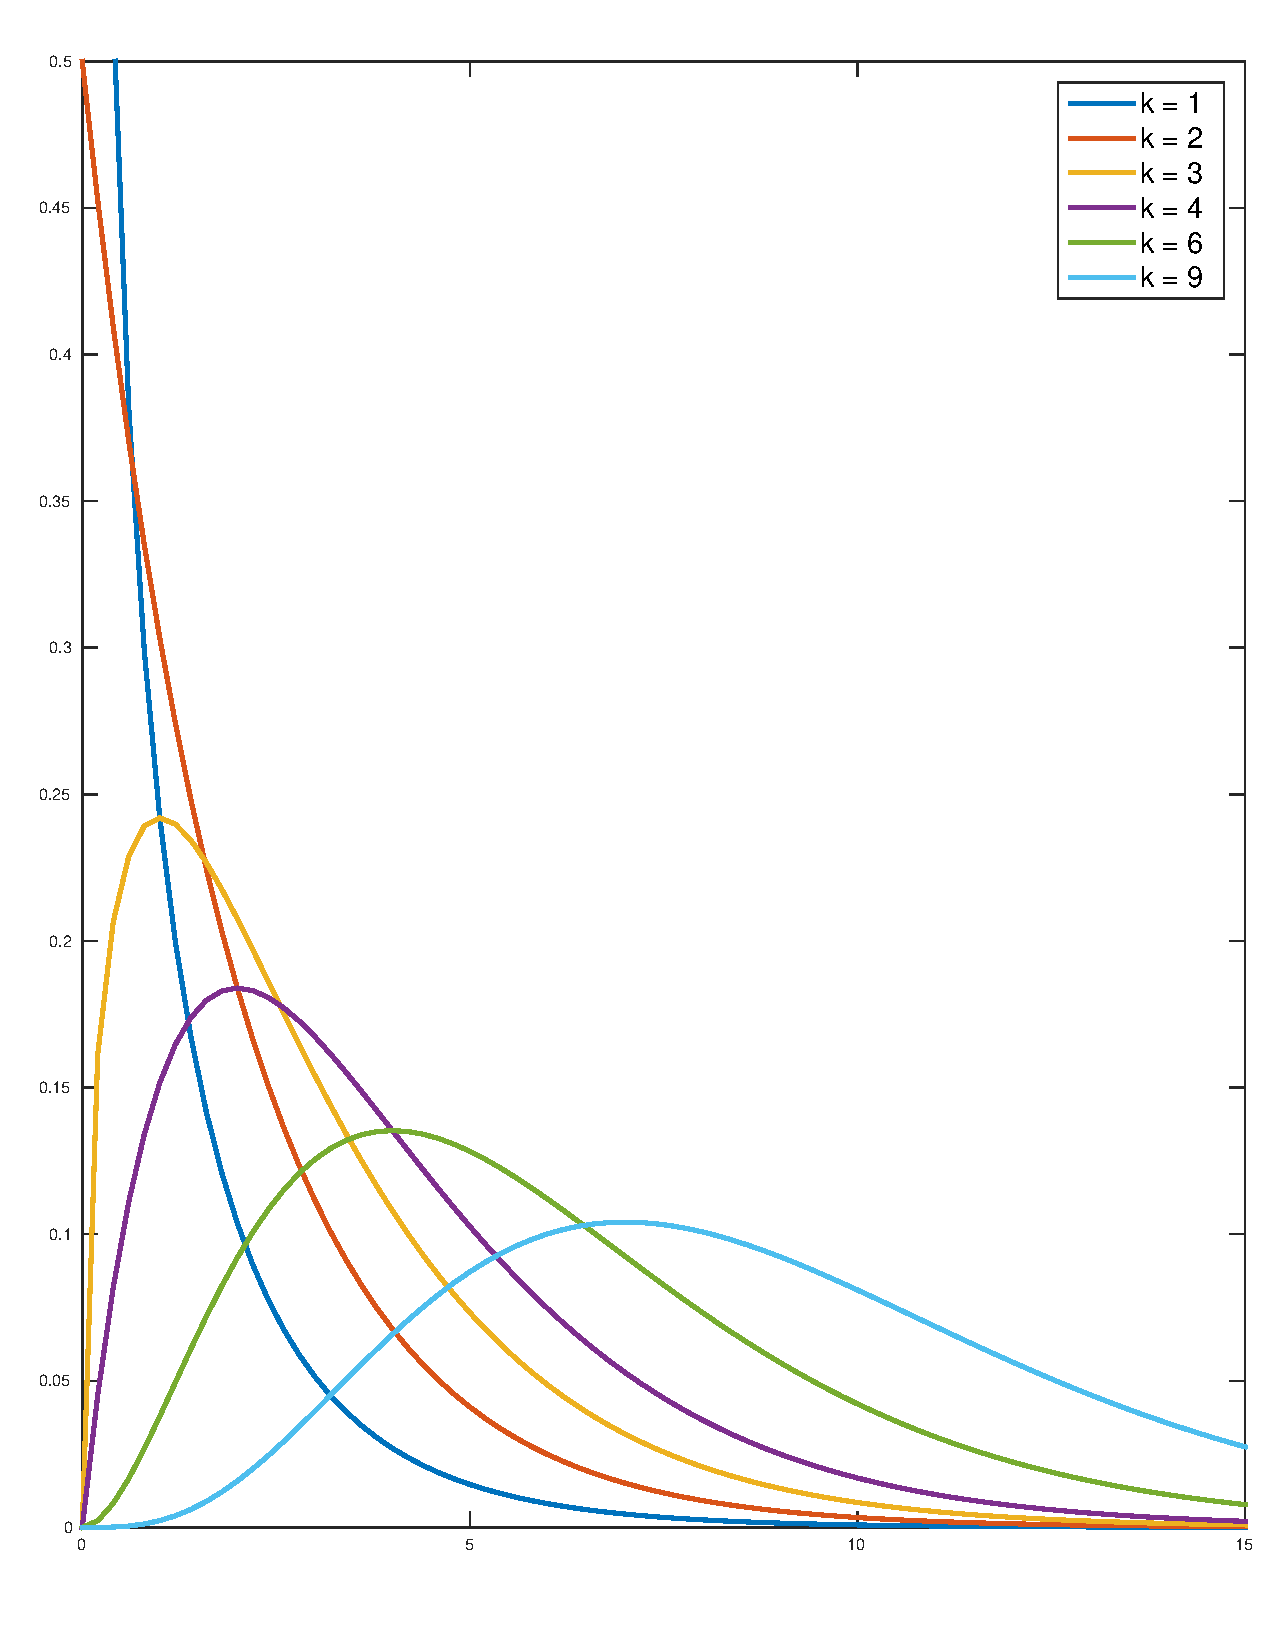
\includegraphics[width=.9\textwidth, height = 12cm]{images/ChiSquareDistribution}
    \caption{Chi-square distribution with different parameters}
    \label{fig:chi-square_distribution}
\end{figure}
\newline
\begin{defn}
\label{defn:chi_square_distribution}
\cite{distribution_cryptanalysis_kaisa_lecture_ice_break_2013} Let $X_i \sim \mathcal{N}(\mu_i,\sigma^2_i)$ where $i = 0, . . . ,k$. Then the random variable
\begin{eqnarray}
T_0 &=& \displaystyle\sum_{i=0}^{k}\frac{(X_i - \mu_i)^2}{\sigma^2_i} 
\end{eqnarray} has central $\chi^2$ distribution with $k$ degrees of freedom which is written as 
\begin{eqnarray}
T_0 &\sim & \chi^2_{k} \label{eqn:chi_square_distribution_central}
\end{eqnarray}
and the random variable 
\begin{eqnarray}
T_1 &=& \displaystyle\sum_{i=0}^{k}\frac{(X_i)^2}{\sigma^2_i} 
\end{eqnarray} has non-central $\chi^2$-distribution with $k$ degrees of freedom where the non-centrality parameter is
\begin{eqnarray}
\delta &=& \displaystyle\sum_{1=0}^{k}\frac{\mu_i^2}{\sigma_i^2} \label{eqn:chi_square_non_centrality}
\end{eqnarray} And this is written as:
\begin{eqnarray}
T_1 &\sim & \chi^2_{k}(\delta) \label{eqn:chi_square_distribution_non_central}
\end{eqnarray}
The mean and variance of the variable $T_0$ which is centrally $\chi^2$-distributed are following:
\begin{eqnarray}
\mu_{T_0} &=& k \label{eqn:chi_square_central_mean}\\
\sigma^2_{T_0} &=& 2k \label{eqn:chi_square_central_variance} 
\end{eqnarray} And the mean and variance of the variable $T_1$ which is non-centrally $\chi^2$-distributed with $\delta$ as non-central parameter is following:
\begin{eqnarray}
\mu_{T_1} &=& k + \delta \label{eqn:chi_square_non_central_mean}\\
\sigma^2_{T_1} &=& 2(k + 2\delta) \label{eqn:chi_square_central_mean}
\end{eqnarray}
\end{defn}
\subsection{Link Between $\chi^2$ and $\Gamma$ Distribution}
A $\chi^2$ variable $X$ of $k$ degrees of freedom is gamma distributed with shape $\alpha = \frac{k}{2}$ and scale $\beta=2$ \citep{chi_gamma_link_book}. That is
\begin{eqnarray}
X \sim \chi^2_{k} \Rightarrow X \sim \Gamma \left(\alpha= k/2, \beta= 2 \right) \label{eqn:link_chi_gamma}
\end{eqnarray}

%Consequently, as $nk \to \infty$, we have
% \begin{eqnarray*}
% \bar X &=& \frac{1}{n} \sum_{i=1}^{n} X_i \sim \Gamma \left(\alpha= nk/2, \beta= 2/n \right) \\
%\Rightarrow \bar X  &\sim & \mathcal{N}\left(\mu = \left(nk/2\right)\left(2/n\right), %\sigma^2 = \left(nk/2\right)\left(2/n\right)^2 \right)\\
%\Rightarrow \bar X  &\sim & \mathcal{N}\left(\mu = k, \sigma^2 = 2k/n \right) 
%\end{eqnarray*}
%So, if we set $n=1$ then for sufficiently large degree of freedom $k$ of a $\chi^2$-%distributed random variable $X$ we have
%\begin{eqnarray}
%X \sim \mathcal{N}\left(k,2k \right) \label{eqn:gamma_dist_property_normal_approximations}
%\end{eqnarray}

\subsection{Normal approximation of $\chi^2$ distribution:} \label{section:normal_approximation_of_chi_square_distribution}
\citep{chi_square_normal_approximation} For large number of degrees of freedom $k$, the chi-square distribution may be approximated by a normal distribution. Consequently we have the following two approximations.
\begin{enumerate}
\item For a sufficiently large value of $k$, a central $\chi^2$-distributed random variable $X$ with $k$ degrees of freedom is approximately normally distributed
\begin{eqnarray}
X \sim \mathcal{N}\left(k,2k \right) \label{eqn:chi_square_central_normal_approx}
\end{eqnarray}
\item For a sufficiently large value of $k$, a non-central $\chi^2$-distributed random variable $X$ with $k$ degrees of freedom and $\delta$ as non-centrality parameter is approximately normally distributed
\begin{eqnarray}
X \sim \mathcal{N}\left(k+\delta,2 \left(k+ 2\delta \right) \right) \label{eqn:chi_square_non_central_normal_approx}
\end{eqnarray}
\end{enumerate}


\subsection{Normal approximation of $\Gamma$ Distribution} \label{section:link_gamma_normal_distribution}
Let the shape and scale parameters of a gamma distribution be $\alpha$ and $\beta$. Asymptotically, given that for a shape parameter $\alpha$,  going to infinity, a gamma distribution converges towards a normal distribution with expectation  $\mu = \alpha\cdot \beta$ and variance  $\sigma^2 = \alpha\, \beta^2$ \cite{normal_approximation_of_gamma_distribution_uah}.

\subsection{Binomial Distribution}
As defined in \cite{binomial_distribution_defn}, the binomial distribution with parameters $n$ and $\theta$ is the discrete probability distribution of the number of successes in a sequence of $n$ independent ``$yes/no$'' experiments, each of which yields success with probability $\theta$. The probability of getting exactly $k$ successes in $n$ trials is given by the probability mass function
\begin{eqnarray}
f(k;n,\theta) = \Pr(X = k) = {n\choose k}\theta^k(1-\theta)^{n-k} \label{eqn:binomail_distribution_pmf}
\end{eqnarray}
for $k = 0, 1, 2, ..., n$, where ${n\choose k}=\frac{n!}{k!(n-k)!}$ is the binomial coefficient, hence the name of the distribution. \par \noindent Let $N$ be the number of data (sample size), $M$ be the number of cells with different probabilities $p(\eta), \eta = 1, 2, . . . , M$. Now if $\omega(\eta)$ denotes the number of data in cell $\eta$, then
$\omega(\eta) \sim \mathcal{B}(p(\eta))$. As mentioned in \cite{distribution_cryptanalysis_kaisa_lecture_ice_break_2013}, for large $N$ we have 
\begin{eqnarray}
\omega(\eta) \sim \mathcal{N}(Np(\eta), Np(\eta)) \approx \mathcal{N}(Np(\eta), N/M) \label{eqn:binomial_distribution_normal_approximation}
\end{eqnarray}

\section{Capacity}
\subsection{Capacity of a Distribution} \label{section:capacity_of_a_distribution}
Given a function $f:X \rightarrow Y$, $x \in X$, $\eta \in Y$, and $X$ is uniformly distributed, the probability of $f(x) =\eta$ is denoted by $p_{\eta}$ defined as 
\begin{eqnarray}
p_{\eta} = |X|^{-1}\#\lbrace x \in X \;|\; f(x) = \eta \rbrace \label{eqn:p_eta_a}
\end{eqnarray}  
The probability distribution of the function $f$ is described by the pmf $p = (p_{\eta})$. The uniformity of a distribution $p$ is measured by its capacity, also called as Squared Euclidean Imbalance. Capacity of a distribution is computed from its squared distance from the uniform distribution. If the capacity of a distribution $p$ is denoted by $C_p$, then it can be formally written as 
\begin{eqnarray}
C_{p} = |Y|\displaystyle\sum_{\eta \in Y}(p_{\eta} - |Y|^{-1})^2 \label{eqn:capacity_of_a_distribution}
\end{eqnarray}Let $p(a) = (p_{\eta}(a))$ denote a probability distribution over domain $Y$ in a family of distributions parametrized by $a \in I$. We consider $a$ as a uniformly distributed random variable. We assume that this family of probability distributions satisfies the following hypothesis. 
\begin{hyp}\label{hyp:hypothesis_on_p_eta_a}
For each fixed $\eta \in Y$, the probability $p_{\eta}(a)$ is a random variable and independently distributed and follow the normal distribution
\begin{eqnarray*}
p_{\eta}(a) \sim \mathcal{N}\left(\mu,\sigma^2\right) 
\end{eqnarray*}
where $\mu = |Y|^{-1}$
\end{hyp}For an arbitrarily fixed $a$, the capacity of $p(a) = \left(p_{\eta}\left(a\right)\right)$ is denoted by $C(a)$. Then
\begin{eqnarray}
C\left(a\right) = |Y|\displaystyle\sum_{\eta \in Y}(p_{n}\left(a\right) - |Y|^{-1})^2 \label{eqn:defn_c(a)}
\end{eqnarray}
The average capacity over the parametrized probability distributions $p(a)$ is defined by 
\begin{eqnarray}
C = |I|^{-1}\displaystyle\sum_{a \in I}C(a) \label{eqn:average of C a}
\end{eqnarray}
\subsection{Distribution of Capacity}
\begin{theorem}\label{general capacity distribution}
Given a family $p(a), a \in I$ of probability distributions that satisfies Hypothesis 1, the capacity $C(a)$ is gamma distributed $$C(a) \sim \Gamma\left(\frac{|Y|-1}{2},\frac{2C}{|Y|-1}\right)$$ with mean $C$ and variance $\frac{2C^2}{|Y|-1}$
\end{theorem}
\begin{proof}
Let $\mu_{C(a)}$ and $\sigma^{2}_{C(a)}$ denote the mean and variance of $C(a)$ respectively. According to (\ref{eqn:average of C a}) we have $\mu_{C(a)} = C$. Let us now examine the parametrized statistic $Q(a)$ defined as
\begin{eqnarray}
Q(a) &=& \displaystyle\sum_{\eta}\frac{\left(p_{\eta}(a) - \mu_{p_{\eta}(a)}\right)^2}{\sigma^{2}_{p_{\eta}(a)}} 
\end{eqnarray}
From Hypothesis \ref{hyp:hypothesis_on_p_eta_a}, we know that $p_{\eta}(a)$ is identically and independently normally distributed. As a result, using Hypothesis \ref{hyp:hypothesis_on_p_eta_a} and Definition  \ref{defn:chi_square_distribution}, we can write
\begin{eqnarray}
Q\left(a\right) &=& \displaystyle\sum_{\eta}\frac{(p_{\eta}(a) - |Y|^{-1})^2}{\sigma^{2}} \sim  \chi^2_{|Y|-1} \label{eqn:Q(a)}
\end{eqnarray}
Let us multiply both sides of (\ref{eqn:Q(a)}) by the cardinality of the set $Y$ and variance of the distribution $p_{\eta}(a)$.  The result is following:
\begin{eqnarray}
|Y|Q(a)\sigma^{2} &=& |Y|\displaystyle\sum_{\eta}\left(p_{\eta}(a) - |Y|^{-1}\right)^2 \label{eqn:Y_Q_sigma}
\end{eqnarray}
As per definition of capacity of a distribution given in (\ref{eqn:capacity_of_a_distribution}), the right hand side of (\ref{eqn:Y_Q_sigma}) is the capacity of the distribution $p(a)$, which can be denoted as $C(a)$ as per our convention. So, we get
\begin{eqnarray*}
C(a) &=& |Y|\sigma^{2}Q(a)
\end{eqnarray*}
Now if we plug (\ref{eqn:Q(a)}) in (\ref{eqn:link_chi_gamma}), then we can write 
\begin{eqnarray}
Q(a) &\sim& \Gamma\left(\frac{|Y-1|}{2},2\right) \label{eqn:Q_gamma_distributed}
\end{eqnarray}
We see $|Y|$ is a constant and as per Hypothesis \ref{hyp:hypothesis_on_p_eta_a}, $\sigma^2$ is also a constant. According to (\ref{eqn:Q_gamma_distributed}), $Q(a)$ is gamma distributed. So, as per the property of gamma distribution given in (\ref{eqn:gamma_dist_property_scaling}), we can write 
\begin{eqnarray} 
C(a) &\sim & \Gamma\left(\frac{|Y-1|}{2},2|Y|\sigma^{2}\right) \label{eqn:distribution_of_C_a}
\end{eqnarray}
Let us denote the mean of $C(a)$ over all $a \in I$ by $C$. As per the property of gamma distribution given in (\ref{eqn:mean_gamma_dist}) the mean of the gamma distributed random variable is the multiplication of its shape and scale parameter. Consequently, from (\ref{eqn:distribution_of_C_a}), the mean  $C$ is as follows
\begin{eqnarray*}
C &=& |Y-1||Y|\sigma^2\\
\end{eqnarray*} Which implies that
\begin{eqnarray}
\sigma^2 &=& \frac{C}{|Y-1||Y|} \label{eqn:variance_of_p_eta_i}
\end{eqnarray} 
Now by plugging the $\sigma^2$ from (\ref{eqn:variance_of_p_eta_i}) in (\ref{eqn:distribution_of_C_a}), we obtain the following result 
\begin{eqnarray}
C(a) \sim \Gamma\left(\frac{|Y|-1}{2},\frac{2C}{|Y|-1}\right) \label{eqn:distribution_of_C a_second}
\end{eqnarray}
The first claim of the theorem is now proven and it remains to show that the variance is $\sigma^2_{C(a)} = \frac{2C^2}{Y-1}$. As per the property of gamma distribution given in (\ref{eqn:variance_gamma_dist}), variance of a gamma distributed variable  is the multiplication of it's shape parameter and the square of scale parameter. Using this property in (\ref{eqn:distribution_of_C a_second}), we find the variance $\sigma^2_{C(a)}$ as follows 
\begin{eqnarray*}
\sigma^{2}_{C(a)} &=& \frac{|Y-1|}{2}\left(\frac{2C}{|Y-1|}\right)^2 \\ 
&=& \frac{2C^2}{|Y|-1}
\end{eqnarray*}
\end{proof}

\section{A statistical test to distinguish distribution} \label{section:statistical_test} In the applications of cryptanalysis, the task is to distinguish between cipher and random behavior based on an observed distribution computed from sample data. Now we present a statistical test to accomplish this task. To perform the statistical test, we are in need of a statistic computed from the cipher data distribtuion. We denote this statistic as $T$. For the statistical test we are presenting here, it is essential for $T$ to be defined in a way that it is normally distributed. Suppose we already know two normal deviates $T_0$ and $T_1$ such that
\begin{eqnarray*}
T_0 \sim \mathcal{N}\left(\mu_{T_0},\sigma^{2}_{T_0} \right)\\
T_1 \sim \mathcal{N}\left(\mu_{T_1},\sigma^{2}_{T_1} \right)
\end{eqnarray*} and assuming without loss of generality that $\mu_{T_0} < \mu_{T_1}$. Given a $T$ computed from a sample about which we know that it follows either the distribution of $T_0$ or $T_1$. The task is to decide which of those two it is. The test is defined by a value $\tau$. If $T\leq \tau$ the outcome of the test is that $T$ is drawn from the distribution of $T_0$ and if $T > \tau$ then $T$ is drawn from the distribution $T_1$. The error probabilities are defined as 
\begin{eqnarray*}
\alpha_0 &=& \Pr\left(T_0\;|\;T > \tau\right)\\
\alpha_1 &=& \Pr\left(T_1\;|\;T \leq \tau \right)
\end{eqnarray*}
That is, $\alpha_0$ is the probability that the test outputs $T_1$ when the reality is $T_0$. Similarly $\alpha_1$ is the probablity that the test outputs $T_0$ when the reality is $T_1$. To make the error probabilities less than $\alpha_0$ and $\alpha_1$, we must select $\tau$ to satisfy
\begin{eqnarray}
\mu_{T_0} + \sigma_{T_0}\zeta_0 \leq \tau \leq \mu_{T_1} - \sigma_{T_1}\zeta_1 \label{eqn:selecting_tau_range}
\end{eqnarray} where $\mathit{\Phi}(\zeta_i) = 1 - \alpha_i$ for $i \in \mathbb{Z}_2$ for the cumulative distribution function $\mathit{\Phi}$ of the standard normal distribution. That is, $\zeta_i$ indicates how many standard deviation beyond the mean is required to bound the probability of wrongly choosing $T_{i-1}$ by at most $\alpha_i$. The Figure \ref{fig:single_tau_range} shows the range of feasible values of $\tau$. In Figure \ref{fig:single_tau} shows how to choose a single value of $\tau$. Note that in Figure \ref{fig:single_tau}, the area on the right side of the yellow line under the red curve indicates $\alpha_0$ and the area on the left side of the yellow line under the blue curve indicates $\alpha_1$
\begin{figure}[h!]
    \centering
    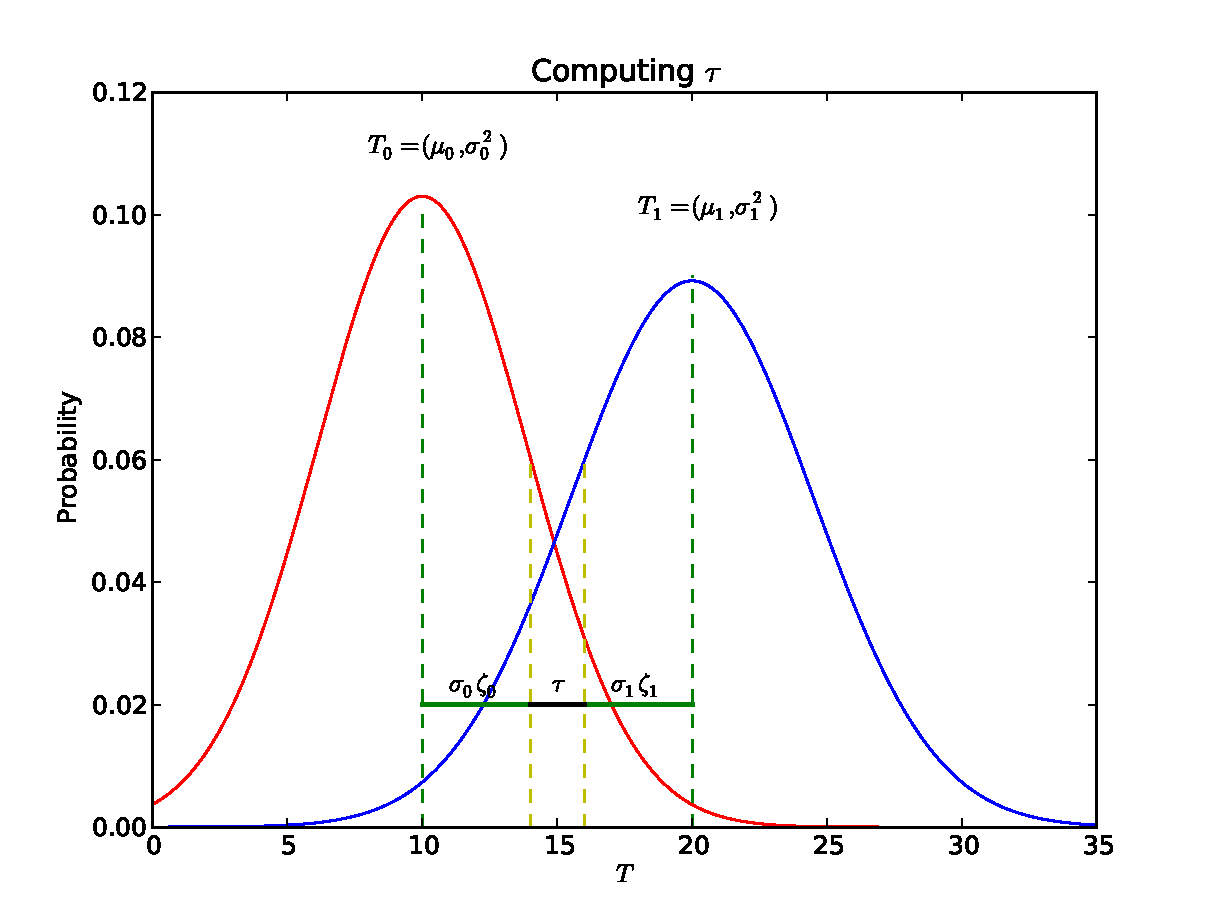
\includegraphics[width=\textwidth , height = 8cm]{images/feasible_range_of_tau}
    \caption{Choosing a range of feasible values of $\tau$}
    \label{fig:single_tau_range}
\end{figure}
In the applications of cryptanalysis the distribution of $T_1$ is determined by the cipher while $T_0$ represents random behaviour. If the cipher distribution has non-zero capacity the statistic $T$ given above can be used. The parameters of $T_1$ depend on the number $N$ of plaintexts, while the parameters of $T_0$ are constant with $N$ as the distribution is uniform and its capacity is equal to zero. Then the distributions of $T_0$ and $T_1$ move apart as $N$ grows. The phenomenon is presented in Figure \ref{fig:single_tau_as_distributions_distinguishes}. In this figure, the blue line has moved on the right along the $X$-axis, which has made the error areas smaller. Then the above equation allows to determine the sample size $N$ which is sufficient to find a threshold $\tau$ that gives a test with as small non-zero error probabilities $\alpha_0$ and $\alpha_1$ as desired.
\begin{figure}[h!]
    \centering
    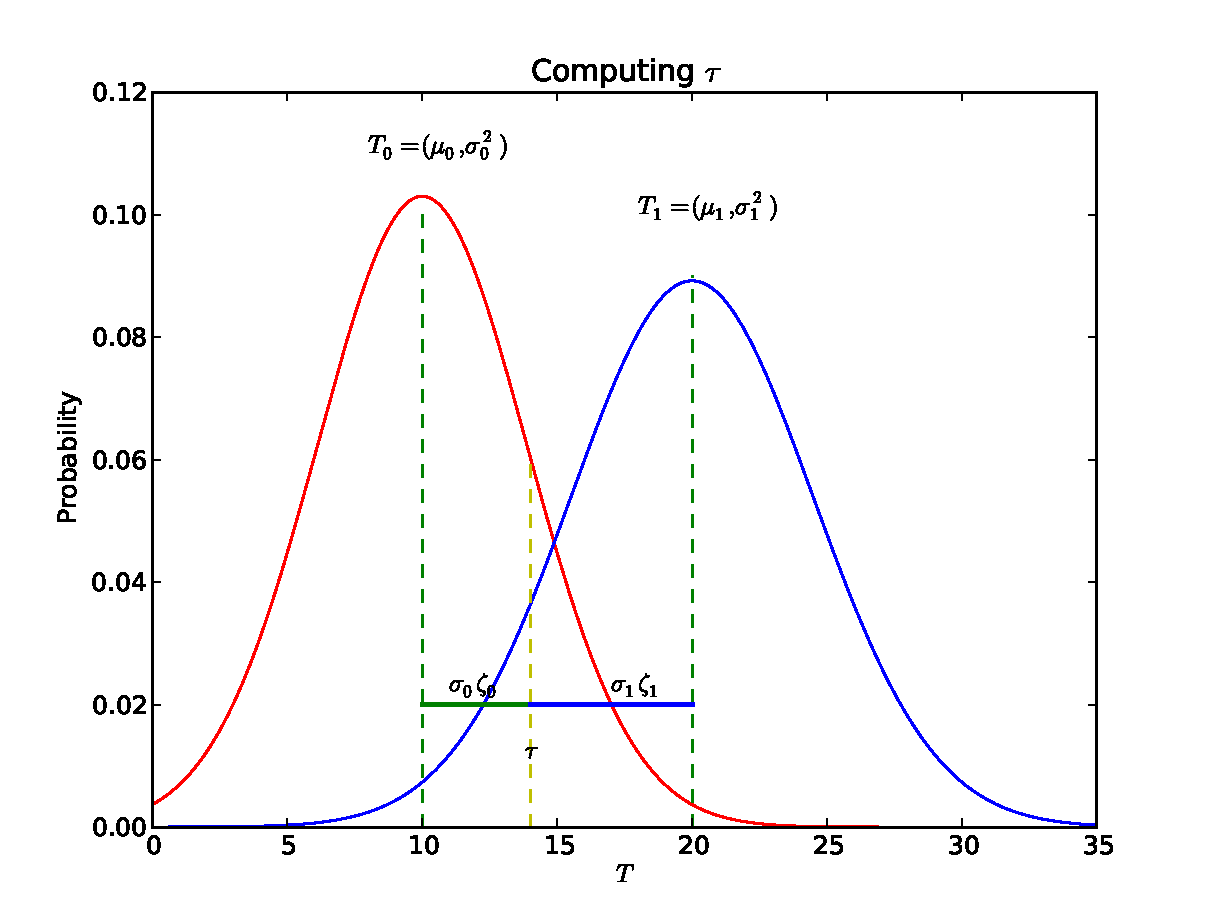
\includegraphics[width=\textwidth , height = 8cm]{images/single_tau}
    \caption{Choosing a single value of $\tau$. That is $\mu_0+\sigma_0\zeta_0 = \mu_1 - \sigma_1\zeta_1$}
    \label{fig:single_tau}
\end{figure}
\begin{figure}[h!]
    \centering
    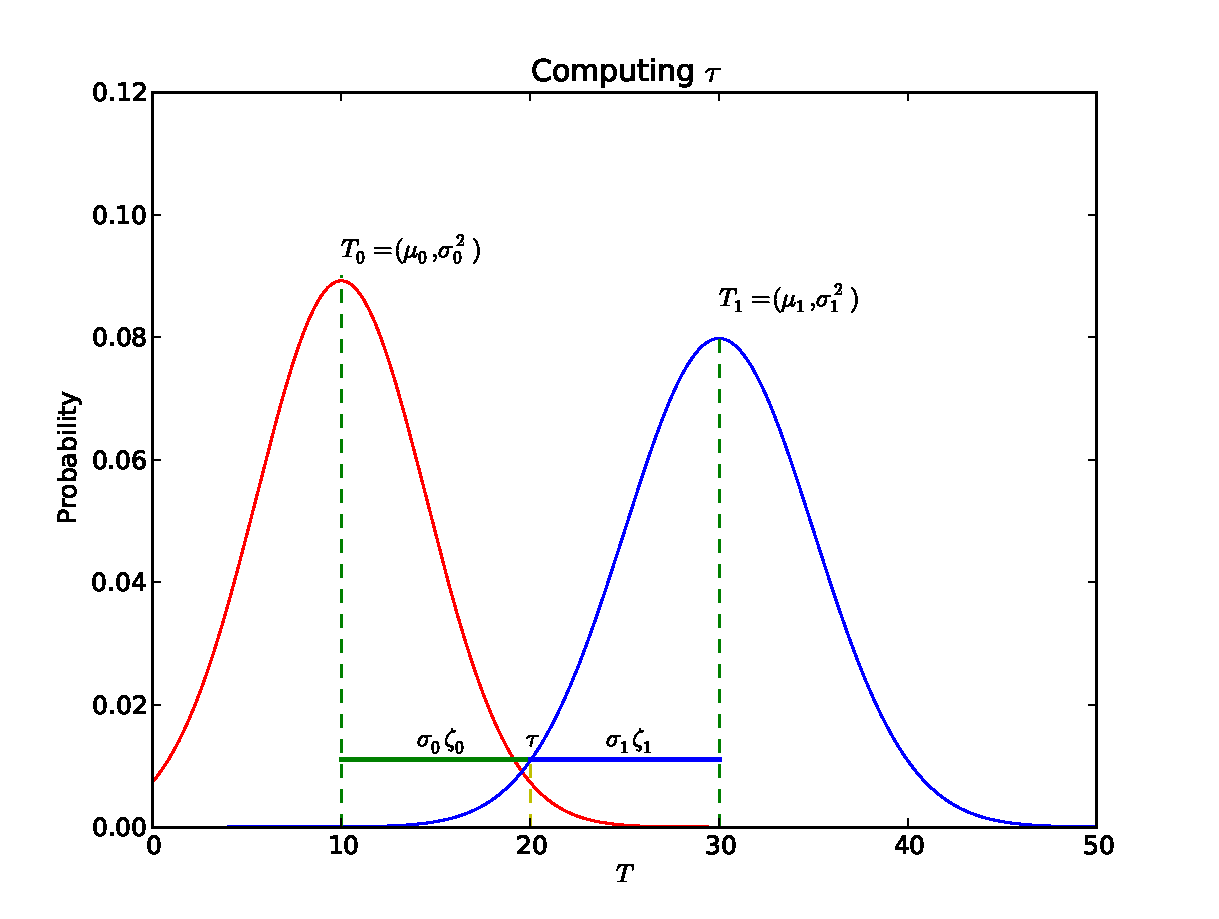
\includegraphics[width=\textwidth , height = 8cm]{images/single_tau_as_the_distributions_distinguishes}
    \caption{As $T_0,T_1$ move apart, $\tau$ can be chosen for smaller error rate}
    \label{fig:single_tau_as_distributions_distinguishes}
\end{figure}
\par \noindent In Section \ref{section:statistic_T}, we have defined statistic $T$ which we have used to develop the statistical model in the Chapter \ref{chapter:statistical_distinguishers}.

\section{Statistic $T$ for the statistical test} \label{section:statistic_T}
We already have mentioned that statistic $T$ is computed from cipher data distribution. Note that the cipher data is computed from a set of chosen plaintexts. Let us call this set of chosen plaintexts as sample denoted by $\phi$. Let us consider a fuction $\Omega:\phi \rightarrow Y$ derived from the encryption function. Let $\omega:Y \rightarrow \mathbb{Z}$ another function such that $\omega\left(\eta \right)$ is the number of times a value $\eta \in Y$ is observed as the output of function $\Omega$, that is
\begin{eqnarray*}
\omega\left( \eta \right) = \# \left\lbrace x \in \phi \; \vert \; \Omega \left( x \right) = \eta \right\rbrace , \eta \in Y
\end{eqnarray*}
Now given a sample $\phi$ of size $N$, we define $T$ as following:
\begin{eqnarray*}
T&=&\displaystyle\sum_{\eta \in Y}\frac{\left( \omega(\eta) - N|Y|^{-1}\right)^2}{N|Y|^{-1}} \\ 
\end{eqnarray*} In sections \ref{section:sampling_with_replacement} and \ref{section:sampling_without_replacement}, we have discussed how the statistic $T$ is distributed when the sample $\phi$ is sampled with or without replacement. 

\subsection{Sampling with replacement} \label{section:sampling_with_replacement} Let $p_{\eta}$ denote the expected probability of getting $\Omega(x) = \eta$ when $N=1$. We also observe that that $\omega({\eta})$ is binomially distributed. As per property of binomial distribution given in (\ref{eqn:binomial_distribution_normal_approximation}) we can write 
\begin{eqnarray}
\mu_{\omega({\eta})} = Np_{\eta} \\
\sigma^2_{\omega({\eta})} = N|Y|^{-1}
\end{eqnarray}
Now, according to the definition of $\chi^2$-distribution given in (\ref{eqn:chi_square_distribution_non_central}), the statistic
\begin{eqnarray*}
T&=&\displaystyle\sum_{\eta \in Y}\frac{\left( \omega(\eta) - N|Y|^{-1}\right)^2}{N|Y|^{-1}} \\ 
&=& \displaystyle\sum_{\eta \in Y}\frac{\left( \omega(\eta) - N|Y|^{-1}\right)^2}{\sigma^2_{\omega({\eta})}}\\
&=& \displaystyle\sum_{\eta \in Y}\frac{\left( \omega(\eta) - N|Y|^{-1}\right)^2}{\sigma^2_{\omega({\eta})- N|Y|^{-1}}}
\end{eqnarray*}
is non-centrally $\chi^2_{|Y|-1}(\delta)$-distributed. To calculate the the non-central parameter $\delta$, we need to know the mean and variance of $\omega(\eta) - N|Y|^{-1}$. Observe that $N|Y|^{-1}$ is a constant and the mean of $\omega(\eta)$ is $Np_{\eta}$. Consequently the mean of $\omega(\eta) - N|Y|^{-1}$ is $Np_{\eta} -N|Y|^{-1}$. And variance of $\omega(\eta)$ and $\omega(\eta) - N|Y|^{-1}$ are same. As a result we can calculate $\delta$ as following
\begin{eqnarray*}
\delta &=& \displaystyle\sum_{\eta \in Y} \frac{\left(Np_{\eta} -N|Y|^{-1} \right)^2}{\sigma^2_{\omega({\eta})- N|Y|^{-1}}}\\
&=& \displaystyle\sum_{\eta \in Y} \frac{N^2\left(p_{\eta} -|Y|^{-1} \right)^2}{N|Y|^{-1}}\\
&=& N \displaystyle\sum_{\eta \in Y} \frac{\left(p_{\eta} -|Y|^{-1} \right)^2}{|Y|^{-1}} \\
&=& NC 
\end{eqnarray*}Where $C$ is the capacity of the distribution $p=(p_{\eta})$. Now according to Definition \ref{defn:chi_square_distribution}, the mean and variance of $T$, denote by $\mu_T$ and $\sigma^2_T$ are 
\begin{eqnarray*}
\mu_T &=& |Y| - 1 + NC\\
\sigma^2_T &=& 2\left(|Y| -1 + 2NC\right) 
\end{eqnarray*}According to the normal approximation of $\chi^2$-distribution as mentioned in Section \ref{section:normal_approximation_of_chi_square_distribution} we can write 
\begin{eqnarray}
T &\sim & \mathcal{N} \left( |Y| - 1 + NC, 2\left(|Y| -1 + 2NC\right) \right)
\end{eqnarray}

\subsection{Sampling without replacement} \label{section:sampling_without_replacement}
When $\phi$ is sampled without replacement, the number of different possible samples decreases as the size of the samples increases. The difference between those different samples also decreases as the size of the samples increases. Which implies, as the sample size grows, the value of $T$ also differs small for different samples. As a result, the variance of $T$ decreases. This is indeed, because when we consider the maximum sample size, there is only one possible sample and only one possible value of $T$ resulted from this sample. Which means, in this case $T$ has zero variance. This phenomenon has been taken into account by Blondeau and Nyberg in \citep{sample_without_replacement}. They have introduced a co-efficient $B$ in the computation of the mean and variance of $T$ using sample without replacement. When the sample size is small, $B$ is almost one and as the sample size grows towards the maximum size, $B$ approaches to zero and becomes zero when the sample size is maximum. \par \noindent According to \citep{sample_without_replacement}, we can define $B$ as $\left(1 - \frac{N}{\lvert \phi \rvert_{max}} \right)$. Here $\lvert \phi \rvert_{max}$ is the largest possible size of a valid sample $\phi$. And the mean and variance of $T$ are following:
\begin{eqnarray}
\mu_T &=& \left(\lvert Y \rvert - 1\right)B + NC \\
\sigma^2_T &=& 2\left(\lvert Y \rvert - 1\right)B^2 + 4BNC
\end{eqnarray} \par \noindent In the next chapter we have extended this discussion of $T$ considering the associated trail of the attack. That is, we have defined the function $\Omega$ considering the the encryption function and the SS trail. However, we will only focus on the case of sampling with replacement in the rest of the thesis. Sampling with replacement is already good enough, in real life cryptanalysis. As shown in \citep{sample_without_replacement}, the method of sampling without replacement offers some advantage when the sample size is close to the full codebook. In an upcoming paper \citep{kaisa_mohsin_2015} the statistical model developed in this work has been extended to the case of sampling without replacement.

\chapter{Statistical Distinguishers}
\label{chapter:statistical_distinguishers} In previous chapter we have discussed how to exploit the weakness of a cipher in SSA. Now we know that, to exploit the weakness of a block cipher by SSA, we need to be able to distinguish a distribution from random. It was shown how a statistical test can accomplish this task. We also have explained that we need a statistic to perform the statistical test and have defined the statistic that we have used in the test. While defining the statistic $T$ in previous chapter we have introduced two function $\Omega$ and $\omega$ but have not exactly defined them. In this chapter we define the statistic $T$ specifically by defining the exact mapping of $\Omega$ and $\omega$ .
\par \noindent In the SSA introduced by Collard and Standaert \cite{SSA_Collard_Standaert}, a part of the plaintext is fixed and the distribution of a part of the ciphertext is observed. Let the plaintext be 
\begin{eqnarray*}
x&=&(x_s,x_t) \in \mathbb{F}_{2}^{s} \times \mathbb{F}_{2}^{t}
\end{eqnarray*} and the ciphertext 
\begin{eqnarray*}
y = E(x,K) = (y_q,y_r) \in \mathbb{F}_{2}^{q} \times \mathbb{F}_{2}^{r}
\end{eqnarray*} We fix the $x_s$ part of the plaintexts to different values and observe the distribution of $y_q$ part. We can define the functions $\Omega$ and $\omega$ differently based on how $x_s$ is fixed. In the following sections we will derive different distributions of the statistics $T$ defined differently, based on different variants of the functions $\Omega$ and $\omega$. 
\section{Model For One Fixation} \label{section:model_for_one_fixation}
We find the distribution of the statistic depending on the way the fixation is chosen. First, we derive the distribution for a given fixation $a$ and then we go for general case of any fixation $a \in \mathbb{F}^2_s$. For a fixed $a \in \mathbb{F}_{2}^{s}$ such that $x = (a,x_t)$ and $K \in \mathbb{F}_{2}^{l}$ the vectorial boolean function under consideration is
\begin{eqnarray}
\Omega_{a}: \phi \rightarrow \mathbb{F}_{2}^{q} \mbox{ where } \Omega_{a}(x_t)=y_q
\end{eqnarray} where $y = E\left(\left(a,x_t\right),K\right) = (y_q,y_r)$ and $\phi \subseteq \mathbb{F}_{2}^{t}$ is sampled randomly with replacement. We also define another integer function $\omega_a:\mathbb{F}_2^q \rightarrow \mathbb{Z}$ such that for a given $\eta \in \mathbb{F}_2^q$
\begin{eqnarray}
\omega_a\left(\eta \right) =  \# \left\lbrace \Omega_a\left( x_t \right) = \eta \; \vert \; x_t \in \phi \right\rbrace  \label{eqn:omega_a}
\end{eqnarray}
%where $\_{a}(\eta) = \# \left\lbrace x|x = (a,x_t),x_t \in \phi, y_q = \eta \right\rbrace$. 
\subsection{Arbitrarily Fixed Fixation}
For a fixed fixation $a$ and any sample $\phi \subseteq \mathbb{F}_{2}^{t}$ such that $|\phi| = N \leq 2^t$, the statistic $T$ is denoted by $T_{a}(\phi)$ and defined as
\begin{eqnarray}
T_{a}(\phi) = \displaystyle\sum_{\eta = 0}^{2^q-1} \frac{\left( \omega_{a}(\eta)-N2^{-q}\right)^2}{N2^{-q}} \label{eqn:T_fixed_a_variable_phi}
\end{eqnarray}
We see that $\omega_{a}(\eta)$ is binomially distributed. So, according to (\ref{eqn:binomial_distribution_normal_approximation}), we can write 
\begin{eqnarray*}
\omega_{a}(\eta) \sim \mathcal{N}\left(\mu_{\omega_{\eta}(a)},\sigma^{2}_{\omega_{\eta}(a)}\right)
\end{eqnarray*} where $\mu_{\omega_{a}(\eta)} = Np_{\eta}(a)$ and $\sigma^{2}_{\omega_{a}(\eta)} = N2^{-q}$. Then the random variable $X_{a}(\eta) = \omega_{a}(\eta)-N2^{-q}$  is also approximately normally distributed 
\begin{eqnarray*}
X_{a}(\eta) \sim \mathcal{N}(\mu_{X_{a}(\eta)},\sigma^{2}_{X_{a}(\eta)})
\end{eqnarray*}  where $\mu_{X_{a}(\eta)} = \mu_{\omega_{a}(\eta)} - N2^{-q}$  and $\sigma^{2}_{X_{a}(\eta)} = \sigma^{2}_{\omega_{a}(\eta)}$. Now we can write 
\begin{eqnarray*}
T_{a}(\phi) &=& \displaystyle\sum_{\eta = 0}^{2^q-1} \frac{\left(X_{a}(\eta) \right)^2}{N2^{-q}} \\
&=& \displaystyle\sum_{\eta = 0}^{2^q-1} \frac{\left( X_{a}(\eta) \right)^2}{\sigma^{2}_{X_{a}\left(\eta\right)}} \\
&=& \displaystyle\sum_{\eta = 0}^{2^q-1} \frac{\left(X_{a}(\eta) \right)^2}{\sigma^{2}_{X_{a}\left(\eta\right)}}
\end{eqnarray*} Then by Definition \ref{defn:chi_square_distribution} we can write
\begin{eqnarray}
T_{a}(\phi) &\sim & \chi_{2^q-1}^2(\delta(a))
\end{eqnarray}where $\chi_{2^q-1}^2(\delta(a))$ is the non-central $\chi^2$ distribution with $2^q-1$ degrees of freedom and non-central parameter 
\begin{eqnarray*}
\delta(a) &=& \displaystyle\sum_{\eta = 0}^{2^q-1} \frac{(\mu_{X_{a}(\eta)})^2}{\sigma^{2}_{X_{a}(\eta)}}\\ 
&=& \displaystyle\sum_{\eta = 0}^{2^q-1} \frac{(\mu_{\omega_{a}(\eta)} - \sigma^{2}_{\omega_{a}(\eta)})^2}{\sigma^{2}_{\omega_{a}(\eta)}}\\
&=&\displaystyle\sum_{\eta = 0}^{2^q-1} \frac{(Np_{\eta}(a)-N2^{-q})^2}{N2^{-q}} \\
&=& NC(a)
\end{eqnarray*} Then by Definition \ref{defn:chi_square_distribution}, for each fixed $a$ the mean $\mu_{T_{a}(\phi)}$ and variance $\sigma^2_{T_{a}(\phi)}$ of $T_{a}(\phi)$, as the sample of size $N$ varies, are 
\begin{eqnarray*}
\mu_{T_{a}(\phi)} &=& 2^q -1 + NC(a)\\
\sigma^2_{T_{a}(\phi)} &=& 2(2^q-1+2NC(a))
\end{eqnarray*}
By the normal approximation of $\chi^2$ distribution as given in (\ref{eqn:chi_square_non_central_normal_approx}), we can write:
\begin{eqnarray*}
T_{a}(\phi) &\sim & \mathcal{N}(\mu_{T_{a}(\phi)},\sigma^2_{T_{a}(\phi)})
\end{eqnarray*}
\begin{eqnarray}
T_{a}(\phi) &\sim & \mathcal{N}\left(2^q -1 + NC(a),2(2^q-1+2NC(a)\right) \label{eqn:distribution_of_T_fixed_a_variable_phi}
\end{eqnarray}
\subsection{Variable Fixation}
By Theorem \ref{general capacity distribution}, for any arbitrarily fixed fixation $a \in \mathbb{F}_2^{s}$, the capacity of the distribution $p(a)$ denoted by $C(a)$ is
\begin{eqnarray*}
C(a) \sim \Gamma\left(\frac{|Y|-1}{2},\frac{2C}{|Y|-1}\right)
\end{eqnarray*} where we have assumed that $p\left(a\right)$ satisfies Hypothesis \ref{hyp:hypothesis_on_p_eta_a}. According to the property of gamma distribution as given in \ref{eqn:mean_gamma_dist} and \ref{eqn:variance_gamma_dist}, the mean and variance of $C\left(a\right)$ over all possible $a$ is $C$ and $\frac{2C^2}{|Y|-1}$ respectively. According to the link in between gamma and normal distribution given in Section $\ref{section:link_gamma_normal_distribution}$ we get
\begin{eqnarray}
C(a) \sim \mathcal{N}\left(C,\frac{2C^2}{|Y|-1}\right) \label{normal distribution C a}
\end{eqnarray} We can derive the mean $\mu_{NC(a)}$ and variance $\sigma^{2}_{NC(a)}$ of $NC(a)$. 
\begin{eqnarray*}
\mu_{NC(a)} &=& N\mu_{C(a)} = NC \\
\sigma^{2}_{NC(a)} &=& N^2\sigma^{2}_{C(a)} = N^2\frac{2C^2}{|Y|-1} = \frac{2(NC)^2}{|Y|-1}
\end{eqnarray*}
That implies
\begin{eqnarray}
NC(a) \sim \mathcal{N}\left(NC,\frac{2(NC)^2}{|Y|-1}\right) \label{Distribution of NC(a)}
\end{eqnarray}
\par \noindent We denote by $T\left(\phi,a \right)$ the statistic $T_a\left(\phi\right)$ where fixation $a$ also varies in the same way sample $\phi$ of size $N$ varies. Then we have the following result.
\begin{theorem} \label{theorem: variable fixation}
Let us assume that sample $\phi$ of size $N \leq 2^t$ drawn randomly with replacement with a fixed key and fixation $a$ of $s$ bits of the plaintext and the number $q$ of observed bits in the ciphertext is sufficiently large. If $p\left(a\right)$ satisfies Hypothesis \ref{hyp:hypothesis_on_p_eta_a}, then $T\left(\phi,a\right)$ is approximately normal with mean $\mu_{T\left(\phi,a\right)}$ and variance $\sigma^2_{T\left(\phi,a\right)}$, where
\begin{eqnarray*}
\mu_{T\left(\phi,a\right)} &=& 2^{-s}\displaystyle\sum_{a \in \mathbb{F}_{2}^{s}}\mu_{T_{a}(\phi)} = 2^{q}-1+NC\\
\sigma^2_{T\left(\phi,a\right)} &=& \frac{2}{2^q - 1}\left(2^q -1 + NC\right)^2
\end{eqnarray*}
\end{theorem}
\begin{proof}
For each fixed $a$ and variable sample $\phi$ of size $N$, according to (\ref{eqn:distribution_of_T_fixed_a_variable_phi}) we have 
\begin{eqnarray*}
T_{a}(\phi) &\sim & \mathcal{N}(2^q - 1 + NC(a),2(2^q -1 + 2NC(a)))
\end{eqnarray*}
And according to (\ref{Distribution of NC(a)}) we also have
\begin{eqnarray*}
NC(a) &\sim & \mathcal{N}\left(NC, \frac{2(NC)^2}{(2^q-1)}\right)
\end{eqnarray*} Hence $T\left(\phi,a\right)$ is also a normal deviate. Now we derive the mean $\mu_{T\left(\phi,a\right)}$ and variance $\sigma^2_{T\left(\phi,a\right)}$ of $T\left(\phi,a\right)$. Let $\Phi$ be the set of all possible samples of size $N$. Then with variable fixation $a \in \mathbb{F}_{2}^{s}$ and variable sample $\phi \in \Phi$ where $|\phi|= N$, we can write:
\begin{eqnarray*}
\mu_{T\left(\phi,a\right)} &=& \frac{1}{2^s|\Phi|}\displaystyle\sum_{a \in \mathbb{F}_{2}^s, \phi \in \Phi}T\left(\phi,a\right) \\
&=& \frac{1}{2^s|\Phi|}\displaystyle\sum_{a \in \mathbb{F}_{2}^s}\displaystyle\sum_{\phi \in \Phi}T_{a}(\phi) \\
&=& \frac{1}{2^s}\displaystyle\sum_{a \in \mathbb{F}_{2}^s}\frac{1}{|\Phi|}\displaystyle\sum_{\phi \in \Phi}T_{a}(\phi)\\
&=& \frac{1}{2^s}\displaystyle\sum_{a \in \mathbb{F}_{2}^s}\mu_{T_{a}(\phi)}\\
&=& \frac{1}{2^s}\displaystyle\sum_{a \in \mathbb{F}_{2}^s}2^q -1 + NC(a)\\
&=& 2^q -1 + \mu_{NC(a)}\\
&=& 2^q -1 + NC
\end{eqnarray*}
Let $\mu_{\mu_{T_{a}(\phi)}}$ be the mean of $\mu_{T_{a}(\phi)}$ over all the fixation $a$. That means  $\mu_{T\left(\phi,a\right)} = \mu_{\mu_{T_{a}(\phi)}}$. So we write 
\begin{scriptsize}
\begin{eqnarray*}
T\left(\phi,a\right) - \mu_{T\left(\phi,a\right)} &=& T - \mu_{T_{a}(\phi)} + \mu_{T_{a}(\phi)} - \mu_{\mu_{T_{a}(\phi)}}\\
\left(T\left(\phi,a\right) - \mu_{T\left(\phi,a\right)}\right)^2 &=& \left((T\left(\phi,a\right) - \mu_{T_{a}(\phi)}) + (\mu_{T_{a}(\phi)} - \mu_{\mu_{T_{a}(\phi)}})\right)^2\\
\frac{1}{2^{s}|\Phi|}\displaystyle\sum_{a \in \mathbb{F}_{2}^{s},\phi \in \Phi}(T\left(\phi,a\right) - \mu_{T\left(\phi,a\right)})^2 &=& \frac{1}{2^{s}|\Phi|}\displaystyle\sum_{a \in \mathbb{F}_{2}^{s},\phi \in \Phi}\left((T\left(\phi,a\right) - \mu_{T_{a}(\phi)}) + (\mu_{T_{a}(\phi)} - \mu_{\mu_{T_{a}(\phi)}})\right)^2\\
\sigma^2_{T\left(\phi,a\right)} &=& \frac{1}{2^{s}|\Phi|}\displaystyle\sum_{a \in \mathbb{F}_{2}^{s},\phi \in \Phi}\left((T\left(\phi,a\right) - \mu_{T_{a}(\phi)}) + (\mu_{T_{a}(\phi)} - \mu_{\mu_{T_{a}(\phi)}})\right)^2\\
\end{eqnarray*}
\end{scriptsize}
Consequently we find
\begin{tiny}
\begin{eqnarray*}
\sigma^2_{T\left(\phi,a\right)} &=& \frac{1}{2^{s}|\Phi|}\displaystyle\sum_{a \in \mathbb{F}_{2}^{s}}\displaystyle\sum_{\phi \in \Phi}\left((T\left(\phi,a\right) - \mu_{T_{a}(\phi)})^2 + 2(T\left(\phi,a\right) - \mu_{T_{a}(\phi)})(\mu_{T_{a}(\phi)} - \mu_{\mu_{T_{a}(\phi)}})  + (\mu_{T_{a}(\phi)} - \mu_{\mu_{T_{a}(\phi)}})^2 \right)
\end{eqnarray*}
\end{tiny}Let MT denote the the middle term at the right side in the above equation. Now let us analyse MT. $(\mu_{T_{a}(\phi)} - \mu_{\mu_{T_{a}(\phi)}})$ part does not depend on the variable $\phi$ because $\mu_{T_{a}(\phi)}$ is the mean of $T_{a}(\phi)$ over all possible $\phi$ and $\mu_{\mu_{T_{a}(\phi)}}$ is a constant. As a result we can write
\begin{eqnarray*}
MT &=&\frac{1}{2^{s}|\Phi|}\displaystyle\sum_{a \in \mathbb{F}_{2}^{s}}\displaystyle\sum_{\phi \in \Phi} 2(T\left(\phi,a\right) - \mu_{T_{a}(\phi)})(\mu_{T_{a}(\phi)} - \mu_{\mu_{T_{a}(\phi)}})\\
&=& \frac{2}{2^{s}|\Phi|} \displaystyle\sum_{a \in \mathbb{F}_{2}^{s}}(\mu_{T_{a}(\phi)} - \mu_{\mu_{T_{a}(\phi)}}) \displaystyle\sum_{\phi \in \Phi} (T\left(\phi,a\right) - \mu_{T_{a}(\phi)})
\end{eqnarray*}
Observe that for a fixed $a$, $T_{a}\left(\phi\right) = T\left(\phi,a\right)$.As a result we get
\begin{eqnarray*}
MT &=& \frac{2}{2^{s}|\Phi|} \displaystyle\sum_{a \in \mathbb{F}_{2}^{s}}\left(\mu_{T_{a}(\phi)} - \mu_{\mu_{T_{a}(\phi)}}\right) \left( \displaystyle\sum_{\phi \in \Phi} T_a\left(\phi\right) - \displaystyle\sum_{\phi \in \Phi} \mu_{T_{a}(\phi)} \right)\\
\end{eqnarray*}
By the definition of mean we know that $\left( \displaystyle\sum_{\phi \in \Phi} T_a\left(\phi\right) = \displaystyle\sum_{\phi \in \Phi} \mu_{T_{a}(\phi)} \right)$. This implies $MT = 0$. And we can continue deriving the variance of $T\left(\phi,a\right)$ as following.
\begin{eqnarray*}
\sigma^2_{T\left(\phi,a\right)} &=& \frac{1}{2^{s}}\displaystyle\sum_{a \in \mathbb{F}_{2}^{s}}\frac{1}{|\Phi|}\displaystyle\sum_{\phi \in \Phi}(T_{a}(\phi) - \mu_{T_{a}(\phi)})^2  + \frac{1}{2^{s}}\displaystyle\sum_{a \in \mathbb{F}_{2}^{s}}\frac{1}{|\Phi|}\displaystyle\sum_{\phi \in \Phi}(\mu_{T_{a}(\phi)} - \mu_{\mu_{T_{a}(\phi)}})^2\\
&=& \frac{1}{2^{s}}\displaystyle\sum_{a \in \mathbb{F}_{2}^{s}} \sigma^2_{T_{a}(\phi)} + \frac{1}{2^{s}}\displaystyle\sum_{a \in \mathbb{F}_{2}^{s}}\frac{1}{|\Phi|}\displaystyle\sum_{\phi \in \Phi}(2^q -1 + NC(a) - 2^q + 1 - NC)^2\\
&=& \frac{1}{2^{s}}\displaystyle\sum_{a \in \mathbb{F}_{2}^{s}} \sigma^2_{T_{a}(\phi)} + \frac{1}{2^{s}}\displaystyle\sum_{a \in \mathbb{F}_{2}^{s}}\frac{1}{|\Phi|}\displaystyle\sum_{\phi \in \Phi}(NC(a) - NC)^2\\
&=& \frac{1}{2^{s}}\displaystyle\sum_{a \in \mathbb{F}_{2}^{s}} \sigma^2_{T_{a}(\phi)} + \frac{1}{2^{s}}\displaystyle\sum_{a \in \mathbb{F}_{2}^{s}}\sigma^{2}_{NC(a)}\\
&=& \frac{1}{2^{s}}\displaystyle\sum_{a \in \mathbb{F}_{2}^{s}} 2(2^q-1+2NC(a)) + \frac{1}{2^{s}}\displaystyle\sum_{a \in \mathbb{F}_{2}^{s}}\frac{2(NC)^2}{2^q-1}\\
&=& 2(2^q-1+2NC) + \frac{2(NC)^2}{(2^q-1)}\\
&=& \frac{2(2^q-1+2NC)(2^q - 1) + 2(NC)^2}{(2^q-1)}\\
&=& \frac{2((2^q - 1)^2 + 2(NC)(2^q -1) + (NC)^2}{(2^q-1)} \\
&=& \frac{2}{(2^q -1)}(2^q -1 + NC)^2
\end{eqnarray*}
\end{proof}
\par \noindent To justify Hypothesis \ref{hyp:hypothesis_on_p_eta_a} we observe that 
\begin{eqnarray*}
2^{-s}\displaystyle\sum_{a \in \mathbb{F}_{2}^{s}}p_{\eta}(a) = 2^{-q}
\end{eqnarray*} as this probability is the probability of the event $y_q = \eta$ taken over all plaintexts. The variance $p_{\eta}\left(a\right)$ taken over $a$ may not be same for all $\eta \in \mathbb{F}_2^q$. We will see in the Experiment chapter that the variance of ``variance of $p_{\eta}\left( a \right)$ taken over $a$'' taken over $\eta$ is nonzero for any number of rounds. And the experimental and theoretical variance of $C\left(a\right)$ taken over all the possible $a$ also differs by large value. However, interestingly we have found that, this does not affect the distance in between the theoretical and experimental variance of the statistic $T$ as shown in Figures \ref{fig:T_a_phi_variable_a_varible_phi_variable_size_03rounds}, \ref{fig:T_a_phi_variable_a_varible_phi_variable_size_04rounds},
\ref{fig:T_a_phi_variable_a_varible_phi_variable_size_22rounds},
\ref{fig:T_a_phi_variable_a_varible_phi_variable_size_23rounds} for the case of SMALLPRESENT-[$4$]. In an upcoming research paper \citep{kaisa_mohsin_2015}, for SMALLPRESENT-[$8$], we have observed that the experimental variance of $T$ is very larger than the theoretical variance but this happens only when the distinguisher already distinguishes itself from the uniform one. As a result, such a distance in between theory and experiment does not affect our original goal significantly.

\section{Model for Multiple Fixations} \label{section:model_for_multiple_fixations}
Let $A \subseteq \mathbb{F}_{2}^{s}$ be a set of fixations, $\phi \subseteq \mathbb{F}_2^t$ be the sample which is sampled randomly with replacement and $\Phi$ is the set of all possible $\phi$. In this context, the functions $\Omega: A \times \phi \rightarrow \mathbb{F}_2^q$ and $\omega:A \times \mathbb{F}_2^q \rightarrow \mathbb{Z}$ are defined so that
\begin{eqnarray}
\Omega(a,x_t) &=& y_q \\
\omega\left(a,\eta \right) &=&  \# \left\lbrace \Omega\left(a,x_t \right) = \eta \; \vert \; x_t \in \phi \right\rbrace  \label{eqn:omega_a_eta}
\end{eqnarray} where $y = E\left(\left(a,x_t\right),K\right) = (y_q,y_r)$ and $a \in A$
\subsection{A given set of fixations}
For a given set of fixations $|A|=M$ and any sample $\phi$ such that $\lvert \phi \rvert = S \leq 2^t$, the size of the domain of the distribution to be distinguished from random is $M2^q$. The distribution of the function $\omega$ is composed of the probabilities $p_{\left(a,\eta\right)}(A)$. In this context, let the statistic $T$ be denoted by $T_{A}\left(\phi\right)$ is defined as
\begin{eqnarray}
T_{A}(\phi) = \displaystyle\sum_{a \in A}\displaystyle\sum_{\eta \in \mathbb{F}_{2}^{q}} \frac{(\omega(a,\eta) - N2^{-q}M^{-1})^2}{N2^{-q}M^{-1}}
\label{eqn:T_for_a_set_of_fixations}
\end{eqnarray} For simplicity, we restrict the considerations to the case where, for each
fixation, the $q$ bits of the ciphertext is computed for equally many, say $S$, different $x_t \in \mathbb{F}_{2}^{t}$. Then $N = MS$, We also observe that for a given $a$, $w_a\left(\phi\right) = w\left(\phi,a\right)$ and $T_{a}\left( \phi \right) = T\left(\phi,a\right)$. Consequently, and we get 
\begin{eqnarray*}
T_{A}(\phi) &=& \displaystyle\sum_{a \in A}\displaystyle\sum_{\eta \in \mathbb{F}_{2}^{q}} \frac{(\omega(a,\eta) - S2^{-q})^2}{S2^{-q}} \\
&=& \displaystyle\sum_{a \in A}\displaystyle\sum_{\eta \in \mathbb{F}_{2}^{q}} \frac{(\omega_a(\eta) - S2^{-q})^2}{S2^{-q}} \\
&=& \displaystyle\sum_{a \in A}T_{a}(\phi)\\
&=& \displaystyle\sum_{a \in A}T(\phi,a) 
\end{eqnarray*}
By Theorem \ref{theorem: variable fixation}, $T(\phi,a)$ is a normal deviate. And from the above equation we see $T_{A}\left(\phi\right)$ is a summation of $\lvert A \rvert = M$ number of normally distributed random variables. As a result, according to the property of normal distribution $T_{A}\left(\phi\right)$ is also normally distributed and we can write
\begin{eqnarray*}
T_{A}(\phi) &\sim & \mathcal{N}\left(M\mu_{T_{a}(\phi)},M\sigma_{T_{a}(\phi)}^2\right)\\
&=& \mathcal{N}\left(M(2^q-1+SC),M\frac{2(2^q -1 +SC)^2}{(2^q -1)}\right)\\
&=& \mathcal{N}\left(M(2^q-1)+MSC,M\frac{2(2^q -1 +SC)^2}{(2^q -1)}\right)\\
\end{eqnarray*}
Which implies
\begin{eqnarray}
T_{A}(\phi) &\sim & \mathcal{N}\left(M(2^q-1)+NC,\frac{2M(2^q -1 +SC)^2}{(2^q -1)}\right)
\end{eqnarray}But the tools developed in this thesis work offer also an alternative approach to determine the distribution of $T_{A}(\phi)$. Instead of splitting the domain of the distribution of $(a,\eta)$ as a union of subdomains of size $2^q$ we can investigate the distribution over the large domain directly. 
\par \noindent Let the capacity of the distribution $p\left(A\right) = \left( p_{\left(a,\eta \right)} \left(A\right) \right)$ be denoted by $C\left(A\right)$. We can now define $C\left(A\right)$ in the same way $C\left(a\right)$ is defined for the distribution $p\left(a\right) = \left( p_{\left(\eta \right)} \left(a\right) \right)$ in \ref{eqn:defn_c(a)} and write
\begin{eqnarray*}
C\left(A\right) = |A|2^q\displaystyle\sum_{\left(a,\eta \right) \in A \times \mathbb{F}_2^q} \left( p_{\left(a,\eta \right)}\left(A\right) - \frac{1}{|A|2^q} \right)^2
\end{eqnarray*}
By plugging in the definition of probability
\begin{eqnarray*}
p_{\left(a,\eta \right)}\left(A\right) = \frac{\#\lbrace x_t \in \mathbb{F}_{2}^{t}\;|\;x_s = a,y_q=\eta \rbrace}{|A|2^t},
\end{eqnarray*} we can write 
\begin{eqnarray}
C\left(A\right) = |A|2^q\displaystyle\sum_{\left(a,\eta \right) \in A \times \mathbb{F}_2^q} \left( \frac{\#\lbrace x_t \in \mathbb{F}_{2}^{t}\;|\;x_s = a,y_q=\eta \rbrace}{|A|2^t} - \frac{1}{|A|2^q} \right)^2 \label{eqn:C(A)_elaborate}
\end{eqnarray}
\begin{lemma} \label{lemma:C(A)} Let us denote by $C(A)$ the capacity of the distribution over the values 
$(a,\eta) \in A \times \mathbb{F}_{2}^{q}$ as $x_t$ varies in $\mathbb{F}_{2}^{t}$. Then 
$$C(A)=\frac{1}{|A|}\displaystyle\sum_{a \in A}C(a)$$
\end{lemma}
\begin{proof}
Let us recall that $C(a)$ is defined in (\ref{eqn:defn_c(a)}) as
\begin{eqnarray}
C(a) &=& 2^q \displaystyle\sum_{\eta \in \mathbb{F}_{2}^{q}}\left(p_{\eta}\left(a\right) -\frac{1}{2^q}\right)^2 \label{eqn:c(a)}
\end{eqnarray}
According to definition $p_{\eta}\left(a\right) = \frac{\#\lbrace x_t \in \mathbb{F}_{2}^{t}\;|\;x_s = a,y_q=\eta \rbrace}{2^t}$. By plugging this equality in \ref{eqn:c(a)}, we continue as following
\begin{eqnarray*}
|A|^{-1}\displaystyle\sum_{a \in A}C(a) &=& |A|^{-1}\displaystyle\sum_{a \in A}2^q \displaystyle\sum_{\eta \in \mathbb{F}_{2}^{q}}\left(\frac{\#\lbrace x_t \in \mathbb{F}_{2}^{t}\;|\;x_s = a,y_q=\eta \rbrace}{2^t} -\frac{1}{2^q}\right)^2\\
&=& |A|^{-1}2^q\displaystyle\sum_{a \in A} \displaystyle\sum_{\eta \in \mathbb{F}_{2}^{q}}\left(\frac{\#\lbrace x_t \in \mathbb{F}_{2}^{t}\;|\;x_s = a,y_q=\eta \rbrace}{2^t} -\frac{1}{2^q}\right)^2\\
&=& |A|^{-1}2^q\displaystyle\sum_{\eta \in \mathbb{F}_{2}^{q}, a \in A}\left(\frac{\#\lbrace x_t \in \mathbb{F}_{2}^{t}\;|\;x_s = a,y_q=\eta \rbrace}{2^t} -\frac{1}{2^q}\right)^2\\
&=& |A|^{-1}2^q\displaystyle\sum_{\eta \in \mathbb{F}_{2}^{q}, a \in A}\frac{|A|^2}{|A|^2}\left(\frac{\#\lbrace x_t \in \mathbb{F}_{2}^{t}\;|\;x_s = a,y_q=\eta \rbrace}{2^t} -\frac{1}{2^q}\right)^2\\
&=& |A|2^q\displaystyle\sum_{\eta \in \mathbb{F}_{2}^{q}, a \in A}\left(\frac{\#\lbrace x_t \in \mathbb{F}_{2}^{t}\;|\;x_s = a,y_q=\eta \rbrace}{|A|2^t} -\frac{1}{|A|2^q}\right)^2
\end{eqnarray*}
Now using (\ref{eqn:C(A)_elaborate}) in the last equality above, we have
\begin{eqnarray*}
|A|^{-1}\displaystyle\sum_{a \in A}C(a) &=& C(A), \mbox{ that is } \\
C(A) &=& \frac{1}{|A|}\displaystyle\sum_{a \in A}C(a)
\end{eqnarray*}
\end{proof}
\begin{lemma} \label{lemma:C(A)_2} Let $A$ be a set of fixations such that $A \subseteq \mathbb{F}_{2}^{s}$ and $|A|=M$ and $C(A)$ be the capacity of the distribution $(a,\eta)$ where $a \in A$ and $\eta \in \mathbb{F}_{2}^{q}$. The average capacity of $C(A)$ as $A$ runs over all possible subset of $\mathbb{F}_{2}^{s}$ such that $|A| = M$ is
$C$ which is also the average capacity of $C(a)$
\end{lemma}
\begin{proof}
Let $\mu_{C(A)}$ denote the average capacity of $C(A)$ and $\mathcal{F}$ be the set family that contains all the $M$-subset of $\mathbb{F}_{2}^{s}$. Then we can write
$$\mu_{C(A)} = \frac{1}{|\mathcal{F}|}\displaystyle\sum_{A \in \mathcal{F}}C(A)$$
Now as per the Lemma \ref{lemma:C(A)} we can write
\begin{eqnarray*}
\mu_{C(A)} &=& \frac{1}{|\mathcal{F}|}\displaystyle\sum_{A \in \mathcal{F}} |A|^{-1}\displaystyle\sum_{a \in A}C(a)\\
&=& \frac{1}{|\mathcal{F}|M}\displaystyle\sum_{A \in \mathcal{F}} \displaystyle\sum_{a \in A}C(a)\\
&=& \frac{1}{|\mathcal{F}|M}\displaystyle\sum_{A \in \mathcal{F}, a \in A}C(a)\\
&=& \frac{1}{|\mathcal{F}|M}\displaystyle\sum_{A \in \mathcal{F}, a \in A}C(a)
\end{eqnarray*} Observe that $|\mathcal{F}| = \binom{2^s}{M}$. As $A$ runs through $\mathcal{F}$ and $a$ runs through each of these $M$-subsets, each term $C\left(a\right)$ for each $a \in \mathbb{F}_2^s$ occurs $\binom{2^s - 1}{M-1}$ many times. So, we can continue with the proof as following
\begin{eqnarray*}
\mu_{C(A)} &=& \frac{\binom{2^s - 1}{M-1}}{\binom{2^s}{M}M}\displaystyle\sum_{a \in \mathbb{F}_2^s}C(a) \\
&=& \frac{1}{2^s}\displaystyle\sum_{a \in \mathbb{F}_{2}^{s}}C(a) \\
&=& C
\end{eqnarray*}

\end{proof}
\begin{corollary} \label{corollary C A}
The capacity $C(A)$ of set $A$ of size $M$ is approximately a normal deviate with mean $\mu_{C(A)} = C$ and variance $\sigma^{2}_{C(A)} = \frac{2C^2}{M(2^q-1)}$
\end{corollary}
\begin{proof}
We know $C\left(a\right)$ is a normal deviate. According to the definition, $C\left(A\right)$ is average of $C\left(a\right)$ over all the $a \in A$. We know that average of a collection of normally distributed random variable is also normally distributed. Consequently $C\left(A\right)$ is a normal deviate. From lemma 2 we see that the mean $\mu_{C(A)} = C$. We know $C\left(A\right) = \frac{1}{|A|}\displaystyle\sum_{a \in A}C\left(a\right)$. So variance of $C\left(A\right)$ will be $\frac{1}{|A|^2}$ times the variance of $\displaystyle\sum_{a \in A}C\left(a\right)$. And variance of $\displaystyle\sum_{a \in A}C\left(a\right)$ is $|A|$ times the variance of $C\left(a\right)$. As a result, we write
\begin{eqnarray*}
\sigma^{2}_{C(A)} &=& \frac{1}{|A|^{2}}|A|\sigma_{C(a)}^{2}\\
&=& \frac{2C^2}{M(2^q-1)}
\end{eqnarray*}
\end{proof}

\begin{corollary} \label{corollary:T_A_phi}
For each fixed set $A \subseteq \mathbb{F}_{2}^{s}$ such that $|A| = M$ and variable sample of size $N = MS$ where $S$ is the size of the sample $\phi \subseteq \mathbb{F}_2^t$ drawn randomly with replacement for each fixation $a \in A$, the statistic $T_{A}(\phi)$ is $\chi^2$-distributed with non-central parameter $\delta(A)=NC(A)$ where degree of freedom is $M2^q-1$. That is
\begin{eqnarray*}
T_{A}(\phi) \sim \chi^2_{M2^{q}-1}(NC(A))
\end{eqnarray*}
\end{corollary}
\begin{proof}
Recall the definition of $T_{A}(\phi)$
\begin{eqnarray*}
T_{A}(\phi) = \displaystyle\sum_{a \in A}\displaystyle\sum_{\eta \in \mathbb{F}_{2}^{q}} \frac{(\omega(a,\eta) - N2^{-q}M^{-1})^2}{N2^{-q}M^{-1}}
\end{eqnarray*}
%$$\implies T_{\phi,a \in A}(A) = \displaystyle\sum_{a \in A}\displaystyle\sum_{\nu \in %\mathbb{F}_{2}^{q}} \frac{(N_{a,\nu}(A) - \frac{N}{2^{q}M})^2}{\frac{N}{2^{q}M}}$$
Here $\omega(a,\eta)$ is non-uniformly binomially distributed. So the mean and variance of $\omega(a,\eta)$ are $\mu_{\omega(a,\eta)} = Np_{\left( a,\eta \right)}\left(A\right)$ and $\sigma^{2}_{\omega(a,\eta)} = \frac{N}{M2^{q}}$. Where $\left( p_{\left(a,\eta\right)\left(A\right)} \right)$ is the probability distribution of function $\omega$. As a result we get
\begin{eqnarray*}
T_{A}(\phi) = \displaystyle\sum_{a \in A}\displaystyle\sum_{\eta \in \mathbb{F}_{2}^{q}} \frac{(\omega(a,\eta) - \mu_{\omega(a,\eta)})^2}{\sigma^{2}_{\omega(a,\eta)}}
\end{eqnarray*} Now let us assume that $X = \omega(a,\eta) - \sigma^{2}_{\omega(a,\eta)}$. Then the mean and variance of $X$ are $\mu_{X} = Np_{\left(a,\eta\right)}(A) - \frac{N}{M2^q}$ and $\sigma^{2}_{X} = \frac{N}{M2^q}$. So we write 
\begin{eqnarray*}
T_{A}(\phi) = \displaystyle\sum_{a \in A,\eta \in \mathbb{F}_{2}^{q}}\frac{(X)^2}{\sigma^{2}_{X}}
\end{eqnarray*} Now as per the definition of non-central $\chi^2$ distribution we see that
\begin{eqnarray*}
T_{A}(\phi) \sim \chi^{2}_{|A|2^q-1}(\delta(A))\\
T_{A}(\phi) \sim \chi^{2}_{M2^q-1}(\delta(A))
\end{eqnarray*} where 
\begin{eqnarray*}
\delta(A) &=& \displaystyle\sum_{a \in A, \eta \in \mathbb{F}_{2}^{q}}\frac{\mu_{X}^2}{\sigma^{2}_{X}}\\
&=& \displaystyle\sum_{a \in A, \eta \in \mathbb{F}_{2}^{q}}\frac{(Np_{\left(a,\eta\right)}(A) - \frac{N}{M2^q})^2}{\frac{N}{M2^q}}\\
&=& NM2^q\displaystyle\sum_{a \in A, \eta \in \mathbb{F}_{2}^{q}}\left(p_{\left(a,\eta\right)}(A) - \frac{1}{M2^q}\right)^2 \\
&=& NM2^q\displaystyle\sum_{a \in A, \eta \in \mathbb{F}_{2}^{q}}\left(\frac{1}{|A|}p_{\left(\eta\right)}(a) - \frac{1}{M2^q}\right)^2 \\
&=& NM\displaystyle\sum_{a \in A} 2^q \displaystyle\sum_{\eta \in \mathbb{F}_{2}^{q}}\left(\frac{1}{|M|}p_{\left(\eta\right)}(a) - \frac{1}{M2^q}\right)^2 \\
&=& NM\displaystyle\sum_{a \in A} \frac{1}{M^2} 2^q \displaystyle\sum_{\eta \in \mathbb{F}_{2}^{q}}\left(p_{\left(\eta\right)}(a) - \frac{1}{2^q}\right)^2 \\
&=& N\frac{1}{|A|}\displaystyle\sum_{a \in A} C\left(a\right) \\
&=& NC(A)
\end{eqnarray*} The last equality is as per Lemma \ref{lemma:C(A)}. That means:
\begin{eqnarray*}
T_{A}(\phi) \sim \chi^{2}_{M2^q-1}(NC(A))
\end{eqnarray*}
\end{proof}\noindent So now as per the property of $\chi^2$-distribution the mean and variance of $T_{A}(\phi)$ are 
\begin{eqnarray}
\mu_{T_{A}(\phi)} &=& M2^q-1+NC(A) \label{eqn:T_A_phi_mean} \\
\sigma_{T_{A}(\phi)}^{2} &=& 2(M2^q-1+2NC(A)) \label{eqn:T_A_phi_variance}
\end{eqnarray}And according to the normal approximation of $\chi^2$-distribution mentioned in Section \ref{section:normal_approximation_of_chi_square_distribution}, we have 
\begin{eqnarray}
T_{A}(\phi) &\sim & \mathcal{N}\left(M2^q-1+NC(A),2(M2^q-1+2NC(A))\right) \label{eqn:T_A_phi_variable_phi_fixed_A}
\end{eqnarray}
where $\phi$ is sampled randomly with replacement.
\subsection{A variable set of fixations}
\begin{lemma} \label{varible set of fixation T phi A}
Now let us consider the statistic $T\left(\phi,A\right)$ where the sample $\phi$ of size $S$ which is sampled randomly with replacement and the set of fixations $A$ of size $M$ both are variable and $N=MS$. Then the mean and variance of $T\left(\phi,A\right)$ are 
\begin{eqnarray*}
\mu_{T\left(\phi,A\right)} &=& M2^q-1 + NC \\
%\sigma^{2}_{T\left(\phi,A\right)} &=& 2(M2^q-1+2N\mu_{C(A)}) + \frac{2(N\mu_{C(A)})^2}{M(2^q-1)}
\sigma^{2}_{T\left(\phi,A\right)} &=& 2(M2^q-1 + 2NC) + N^2\sigma_{C\left(A\right)}^2
\end{eqnarray*}
\end{lemma}
\begin{proof}
Let $\Phi$ is the set of all the $\phi$ with $|\phi|=S$. According to the definition, the mean of $T\left(a,\phi\right)$ over all the possible value of $a$ and $\phi$ is
\begin{eqnarray}
\mu_{T\left(\phi,A \right)} &=& \frac{1}{|\mathcal{F}||\Phi|}\displaystyle\sum_{\phi \in \Phi, A \in \mathcal{F}}T\left(\phi,A\right) \label{eqn:T(a,phi)}
\end{eqnarray}
It is immediate to see that for a given set of fixations $A$, $T\left(\phi,A\right) = T_{A}\left(\phi\right)$. Using this equality in (\ref{eqn:T(a,phi)}), we obtain
\begin{eqnarray*}
\mu_{T\left(\phi,A \right)} &=& \frac{1}{|\mathcal{F}|}\displaystyle\sum_{A \in \mathcal{F}}\frac{1}{|\Phi|}\displaystyle\sum_{\phi \in \Phi}T_{A}\left(\phi\right) \label{eqn:T_phi_A_1}
\end{eqnarray*}
Consequently we can write 
\begin{eqnarray}
\mu_{T\left(\phi,A \right)} &=& \frac{1}{|\mathcal{F}|}\displaystyle\sum_{A \in |\mathcal{F}|}\mu_{T_{A}(\phi)} \label{eqn:T_A_phi_2}\\ 
&=& \mu_{\mu_{T_{A}(\phi)}} \label{eqn:T_A_phi_3}
\end{eqnarray}
Now, by plugging (\ref{eqn:T_A_phi_mean}) in (\ref{eqn:T_A_phi_2}) we obtain
\begin{eqnarray*}
\mu_{T\left(\phi,A \right)} &=& \frac{1}{|\mathcal{F}|}\displaystyle\sum_{A \in |\mathcal{F}|}(M2^q-1+NC(A))\\
&=& \frac{|\mathcal{F}|(M2^q-1)}{|\mathcal{F}|}+\frac{1}{|\mathcal{F}|}\displaystyle\sum_{A \in |\mathcal{F}|}(NC(A))\\
&=& M2^q-1 + N\mu_{C(A)}
\end{eqnarray*}
By applying the Lemma \ref{lemma:C(A)_2} in the last equality above, we can write
\begin{eqnarray}
\mu_{T\left(\phi,A \right)} &=& M2^q-1 + NC
\end{eqnarray}
Using (\ref{eqn:T_A_phi_3}), we can write 
\begin{eqnarray}
T\left(\phi,A\right) - \mu_{T\left(\phi,A\right)} &=& T\left(\phi,A\right) - \mu_{T_{A}(\phi)} + \mu_{T_{A}(\phi)} - \mu_{\mu_{T_{A}(\phi)}} \label{T phi A - mu T phi A}
\end{eqnarray} Taking the average of the square of both side of (\ref{T phi A - mu T phi A}) over all the possible fixations and samples we have 
\begin{eqnarray*}
\sigma^{2}_{T\left(\phi,A\right)} &=& \frac{1}{|\mathcal{F}||\Phi|}\displaystyle\sum_{\phi \in \Phi, A \in \mathcal{F}}(T\left(\phi,A\right) - \mu_{T_{A}(\phi)} + \mu_{T_{A}(\phi)} - \mu_{\mu_{T_{A}(\phi)}})^2
\end{eqnarray*}
By expanding the right side of the above equation we can write
\begin{eqnarray*}
\sigma^{2}_{T\left(\phi,A\right)} &=& \frac{1}{|\mathcal{F}||\Phi|}\displaystyle\sum_{\phi \in \Phi, A \in \mathcal{F}}(T\left(\phi,A\right) - \mu_{T_{A}(\phi)})^2\\
&+& \frac{1}{|\mathcal{F}||\Phi|}\displaystyle\sum_{}(\mu_{T_{A}(\phi)} - \mu_{\mu_{T_{A}(\phi)}})^2 \\
&+& \frac{1}{|\mathcal{F}||\Phi|}\displaystyle\sum_{\phi \in \Phi, A \in \mathcal{F}}2(T\left(\phi,A\right) - \mu_{T_{A}(\phi)})(\mu_{T_{A}(\phi)} - \mu_{\mu_{T_{A}(\phi)}}) \label{eqn:variance_T_A_phi}
\end{eqnarray*}

Let MT denote the the third term at the right side in the above equation. Now let us analyse MT. $(\mu_{T_{A}(\phi)} - \mu_{\mu_{T_{A}(\phi)}})$ part does not depend on the variable $\phi$ because $\mu_{T_{A}(\phi)}$ is the mean of $T_{A}(\phi)$ over all possible $\phi$ and $\mu_{\mu_{T_{A}(\phi)}}$ is a constant. As a result we can write
\begin{eqnarray*}
MT &=& \frac{1}{|\mathcal{F}||\Phi|}\displaystyle\sum_{\phi \in \Phi, A \in \mathcal{F}}2\left( T\left(\phi,A\right) - \mu_{T_{\phi,a}\left(A\right)} \right)\left(\mu_{T_{A}(\phi)} - \mu_{\mu_{T_{A}(\phi)}}\right)\\
&=& \frac{2}{|\mathcal{F}||\Phi|} \displaystyle\sum_{A \in \mathcal{F}}\left(\mu_{T_{A}(\phi)} - \mu_{\mu_{T_{A}(\phi)}}\right) \displaystyle\sum_{\phi \in \Phi} \left(T\left(\phi,A\right) - \mu_{T_{A}(\phi)}\right)
\end{eqnarray*}
Observe that for a fixed $A$, $T_{A}\left(\phi\right) = T\left(\phi,A\right)$.As a result we get
\begin{eqnarray*}
MT &=& \frac{2}{|\mathcal{F}||\Phi|} \displaystyle\sum_{A \in \mathbb{F}_{2}^{s}}\left(\mu_{T_{A}(\phi)} - \mu_{\mu_{T_{A}(\phi)}}\right) \left( \displaystyle\sum_{\phi \in \Phi} T_A\left(\phi\right) - \displaystyle\sum_{\phi \in \Phi} \mu_{T_{A}(\phi)} \right)\\
\end{eqnarray*}
By the definition of mean we know that $\left( \displaystyle\sum_{\phi \in \Phi} T_A\left(\phi\right) = \displaystyle\sum_{\phi \in \Phi} \mu_{T_{A}(\phi)} \right)$. This implies $MT = 0$. And we can continue deriving the variance of $T\left(\phi,A\right)$ as following.
\begin{eqnarray*}
\sigma^{2}_{T\left(\phi,A\right)} &=& \frac{1}{|\mathcal{F}|}\displaystyle\sum_{A \in \mathcal{F}}\frac{1}{|\Phi|}\displaystyle\sum_{\phi \in \Phi}(T_{A}\left(\phi\right) - \mu_{T_{A}(\phi)})^2\\
&+& \frac{1}{|\mathcal{F}||\Phi|}\displaystyle\sum_{\phi \in \Phi, A \in \mathcal{F}}(M2^q-1+NC(A) - M2^q+1-NC)^2
\end{eqnarray*}
By simplifying the right side of the above equation we obtain
\begin{eqnarray}
\sigma^{2}_{T\left(\phi,A\right)} &=& \frac{1}{|\mathcal{F}|}\displaystyle\sum_{A \in \mathcal{F}}\sigma_{T_{A}(\phi)}^{2} + \frac{1}{|\mathcal{F}||\Phi|}\displaystyle\sum_{\phi \in \Phi, A \in \mathcal{F}}(NC(A)-NC)^2 \label{eqn:T_A_phi_variance_2}
\end{eqnarray}
Now by using the (\ref{eqn:T_A_phi_variance}) in (\ref{eqn:T_A_phi_variance_2}) we can continue the derivation as following
\begin{eqnarray*}
\sigma^{2}_{T\left(\phi,A\right)} &=& \frac{1}{|\mathcal{F}|}\displaystyle\sum_{A \in \mathcal{F}}2(M2^q-1+2NC(A)) + \frac{1}{|\mathcal{F}||\Phi|}\displaystyle\sum_{\phi \in \Phi, A \in \mathcal{F}}(NC(A)-NC)^2\\
&=& \frac{1}{|\mathcal{F}|}\displaystyle\sum_{A \in \mathcal{F}}2(M2^q-1)+4NC(A) + \frac{N^2}{|\mathcal{F}||\Phi|}\displaystyle\sum_{\phi \in \Phi, A \in \mathcal{F}}(C(A)-C)^2\\
\end{eqnarray*}
The mean of $C\left(A\right)$ over all possible $A$ is $C$ according to Lemma \ref{lemma:C(A)_2}. So, according to the definition of the variance of any statistic and using the fact that $2\left(M2^q -1 \right),4N$, and $\sigma_{C\left(A\right)}^2$ over all possible $A$  are constant, we can write the following:
\begin{eqnarray*}
\sigma^{2}_{T\left(\phi,A\right)} &=& 2(M2^q-1) + \frac{4N}{|\mathcal{F}|}\displaystyle\sum_{A \in \mathcal{F}} C(A) + \frac{N^2}{|\Phi|}\displaystyle\sum_{\phi \in \Phi}\frac{1}{|\mathcal{F}|}\displaystyle\sum_{A \in \mathcal{F}}(C(A)-C)^2\\
&=& 2(M2^q-1) + \frac{4N}{|\mathcal{F}|}\displaystyle\sum_{A \in \mathcal{F}} C(A) + \frac{N^2}{|\Phi|}\displaystyle\sum_{\phi \in \Phi}\sigma_{C(A)}^{2}\\
&=& 2(M2^q-1)+4NC + N^2\sigma_{C(A)}^{2}\\
&=& 2(M2^q-1+2NC) + N^2\sigma_{C(A)}^{2}
\end{eqnarray*}
\end{proof}Recall that our objective is to find the distribution of the statistic $T$ and in this context, $T\left(a,\phi \right)$. From Lemma \ref{varible set of fixation T phi A}, we can find the mean and variance of $T\left(a,\phi \right)$. And from Corollary \ref{corollary C A}, we find the value of $\sigma_{C(A)}^{2}$. So, by using the corollary in the lemma, we can continue computing the variance of $T\left(a,\phi\right)$ as following
\begin{eqnarray*}
\sigma^{2}_{T\left(\phi,A\right)} &=& 2(M2^q-1+2NC) + N^2\sigma_{C(A)}^{2}\\
&=& 2(M2^q-1+2NC) + \frac{2(NC)^2}{M(2^q-1)}\\
&=& \frac{2(M2^q-M+M-1+2NC)M(2^q-1) + 2(NC)^2}{M(2^q-1)}\\
&=& \frac{2(M(2^q-1)+(M-1)+2NC)M(2^q-1) + 2(NC)^2}{M(2^q-1)}\\
&=&\frac{2((M(2^q-1))^2+M(2^q-1)(M-1)+2NCM(2^q-1))+ (NC)^2}{M(2^q-1)}\\
&=& \frac{2((M(2^q-1))^2+2NCM(2^q-1))+ (NC)^2}{M(2^q-1)}+\frac{2M(2^q-1)(M-1)}{M(2^q-1)}\\
&=& \frac{2(M(2^q-1)+ NC)^2}{M(2^q-1)}+2(M-1)
\end{eqnarray*} As mentioned in Section \ref{section:link_gamma_normal_distribution}, $T_{A}(\phi)$-is approximately normally distributed. Now as $C(A)$ is normally distributed, so is $NC\left(A\right)$. As a result, $T\left(\phi,A\right)$ is also normally distributed. That is
\begin{eqnarray*}
T\left(\phi,A\right) &\sim & \mathcal{N}(\mu_{T\left(\phi,A\right)},\sigma_{T\left(\phi,A\right)}^{2})
\end{eqnarray*}
And consequently
%\begin{scriptsize}
\begin{eqnarray*}
T\left(\phi,A\right) &\sim & \mathcal{N}\left(M2^q-1 + NC,\frac{2(M(2^q-1)+ NC)^2}{M(2^q-1)}+2(M-1)\right) 
\end{eqnarray*}
%\end{scriptsize}
where $\phi$ is sampled randomly with replacement. We observe that for sufficiently large value of $q$, the term $2(M-1)$ is negligibly small in the above variance. And $q$ is always sufficiently large. To simplify the analysis of the data complexity of the distinguisher based on the statistic $T(\phi,A)$ we have used the following approximation
\begin{eqnarray}
T\left(\phi,A\right) &\sim & \mathcal{N}\left(M2^q-1 + NC,\frac{2(M(2^q-1)+ NC)^2}{M(2^q-1)}\right) \label{eqn:T_a_variable_set_of_fixations}
\end{eqnarray}

%\section{Alternative Model for Variable Set of Fixations}
\iffalse
%%%%%%%%%%%%%%%%%%%%%%%%%%%%%%%%%%%%%%%%%%%%%%%%%%%%%%%%%%%%%%%%%%%%%%%%%%%%%%%%%%%
%%%%%%%%%%%%%%%%%%%%%%%%%%%%%%%%%%%%%%%%%%%%%%%%%%%%%%%%%%%%%%%%%%%%%%%%%%%%%%%%%%%
%%%%%%%%%%%%%%%%%%%%%%%%%%%%%%%%%%%%%%%%%%%%%%%%%%%%%%%%%%%%%%%%%%%%%%%%%%%%%%%%%%%
%%%%%%%%%%%%%%%%%%%%%%%%%%%%%%%%%%%%%%%%%%%%%%%%%%%%%%%%%%%%%%%%%%%%%%%%%%%%%%%%%%%
\subsection{First Alternative Model}
\begin{corollary} 
Let $\mathcal{F}$ denotes the set of all the disjoint subsets of $\mathbb{F}_{2}^{s}$ such that $\bigcup A_j = \mathbb{F}_{2}^{s}$ where $A_j \in \mathcal{F}$ and for all $j \neq k$ it holds that $A_j \cap A_k = \emptyset$ and $|A_j|=|A_k|$. Let $p_{\eta}(A_j)$ denotes the probability of getting $y_q = \eta$ where the fixation $a \in A_j$ and $A_j \in \mathcal{F}$. Then $p_{\eta}(A_j)$ is $i.i.d$ for a fixed $\eta$ and variable $A_j \in \mathcal{F}$ and 
\begin{eqnarray*}
p_{\eta}(A_j) &\sim & \mathcal{N}\left(\frac{1}{2^q},\frac{C}{|A_j|2^q(2^q-1)}\right)
\end{eqnarray*}
\end{corollary}
\begin{proof} As per the definition we have
\begin{eqnarray*}
p_{\eta}(A_j) &=& \frac{\# \lbrace (x_s,x_t) \in \mathbb{F}_{2}^{s} \times \mathbb{F}_{2}^{t}|x_s \in A_j, y_q = \eta \rbrace }{|A_j|2^t}
\end{eqnarray*} where $(y_q,y_r) = E_k(x_s,x_t)$. Which means
\begin{eqnarray*}
p_{\eta}(A_j) &=& \displaystyle\sum_{a \in A_j}\frac{\# \lbrace (a,x_t) \in \mathbb{F}_{2}^{s} \times \mathbb{F}_{2}^{t}| y_q = \eta \rbrace }{|A_j|2^t}\\
&=& \frac{1}{|A_j|}\displaystyle\sum_{a \in A_j}\frac{\# \lbrace (a,x_t) \in \mathbb{F}_{2}^{s} \times \mathbb{F}_{2}^{t}| y_q = \eta \rbrace }{2^t}\\
&=& \frac{1}{|A_j|}\displaystyle\sum_{a \in A_j}p_{\eta}(a)
\end{eqnarray*} From Hypothesis 1 we know that $p_{\eta}(a)$ is $i.i.d$ for a fixed $\eta$ and variable fixation $a$. Consequently $p_{\eta}(A_j)$ is $i.i.d$ for a fixed $\eta$ and variable $A_j \in \mathcal{F}$. From Hypothesis 1 we know that 
\begin{eqnarray*}
p_{\eta}(a) \sim \mathcal{N}\left(\frac{1}{2^q},\frac{C}{2^q(2^q-1)}\right)
\end{eqnarray*}where $C$ is the average capacity of the distribution of $y_q \in \mathbb{F}_{2}^{q}$. Consequently 
\begin{eqnarray*}
p_{\eta}(A_j) \sim \mathcal{N}\left(\mu_{p_{\eta}(A_j)},\sigma^{2}_{p_{\eta}(A_j)}\right)
\end{eqnarray*}
where
\begin{eqnarray*}
\mu_{p_{\eta}(A_j)} &=& \frac{1}{|\mathcal{F}|}\displaystyle\sum_{A_j \in \mathcal{F}}p_{\eta}(A_j)= \frac{1}{|\mathcal{F}|}\displaystyle\sum_{A_j \in \mathcal{F}}\frac{1}{|A_j|}\displaystyle\sum_{a \in A_j}p_{\eta}(a)\\
&=& \frac{1}{|\mathcal{F}||A_j|}\displaystyle\sum_{A_j \in \mathcal{F},a \in A_j}p_{\eta}(a)=\frac{1}{2^s}\displaystyle\sum_{a \in \mathbb{F}_{2}^{s}}p_{\eta}(a)\\
&=& \frac{1}{2^q}\\
\sigma^2_{p_{\eta}(A_j)}&=&\sigma^2_{\frac{1}{|A_j|}\displaystyle\sum_{a \in A_j}p_{\eta}(a)} = \frac{1}{|A_j|^2}\sigma^2_{\displaystyle\sum_{a \in A_j}p_{\eta}(a)}\\
&=&\frac{1}{|A_j|^2}\frac{|A_j|C}{2^q(2^q-1)}=\frac{C}{|A_j|2^q(2^q-1)}
\end{eqnarray*}As a result 
\begin{eqnarray*}
p_{\eta}(A_j) &\sim & \mathcal{N}\left(\frac{1}{2^q},\frac{C}{|A_j|2^q(2^q-1)}\right)
\end{eqnarray*}
\end{proof}
\begin{theorem}
Given a family $p(A_j)$, $A_j \in \mathcal{F}$ of probability distributions the capacity where $\mathcal{F}$ denotes the set of all the disjoint subsets of $\mathbb{F}_{2}^{s}$ such that $\bigcup A_j = \mathbb{F}_{2}^{s}$ where $A_j \in \mathcal{F}$ and for all $j \neq k$ it holds that $A_j \cap A_k = \emptyset$ and $|A_j|=|A_k|$. Then the capacity $C(A_j)$ is distributed as 
\begin{eqnarray*}
C(A_j) &\sim & \mathcal{N}\left(\frac{C}{A_j},\frac{2C^2}{|A_j|^2(2^q -1)}\right)
\end{eqnarray*}
\end{theorem}
\begin{proof}
By the above corollary and definition of $\chi^2$-distribution we obtain that
\begin{eqnarray*}
Q &=& \displaystyle\sum_{\eta}\frac{\left(p_{\eta}(A_j) - \mu_{p_{\eta}(A_j)}\right)^2}{\sigma_{p_{\eta}(A_j)}^2} \sim \chi^{2}_{2^q-1}\\
Q2^q\sigma_{p_{\eta}(A_j)}^2 &=& 2^q\displaystyle\sum_{\eta}\left(p_{\eta}(A_j) - \mu_{p_{\eta}(A_j)}\right)^2\\
C(A_j) &=& Q2^q\sigma_{p_{\eta}(A_j)}^2
\end{eqnarray*}
Now, as we know from the discussion of theoretical background that, $\chi^2$-distribution is a gamma distribution with the shape parameter $\alpha = \frac{\nu}{2}$ and the scale parameter $\beta = 2$ where $\nu$ is the degree of freedom of the $\chi^2$ distribution. Then we can write
\begin{eqnarray*}
Q \sim \Gamma\left(\frac{\left(2^q-1\right)}{2},2\right)
\end{eqnarray*}Now we see $2^q\sigma_{p_{\eta}(A_j)}^2$ is a constant and $Q$ is a Gamma distribution. So as per the property of gamma distribution we can write
\begin{eqnarray*}
C(A_j) &\sim & \Gamma\left(\frac{2^q-1}{2},22^q\sigma_{p_{\eta}(A_j)}^2\right)\\
C(A_j) &\sim & \Gamma\left(\frac{(2^q-1)}{2},22^q\frac{C}{|A_j|2^q(2^q-1)}\right)\\
C(A_j) &\sim & \Gamma\left(\frac{(2^q-1)}{2},\frac{2C}{|A_j|(2^q-1)}\right)
\end{eqnarray*}
Now as per the property of Gamma distribution mentioned in (\ref{eqn:mean_gamma_dist}) and (\ref{eqn:variance_gamma_dist}),the mean $\mu_{C(A_j)}$ and variance $\sigma_{C(A_j)}^2$ of $C(A_j)$ are
\begin{eqnarray*}
\mu_{C(A_j)} &=& \frac{2^q-1}{2}22^q\sigma_{p_{\eta}(A_j)}^2\\
&=& (2^q-1)2^q\sigma_{p_{\eta}(A_j)}^2\\
%(discuss about  $C_{w}(A_j)$ Vs $C(A_j)$)
&=& (2^q-1)2^q\frac{C}{|A_j|2^q(2^q-1)}\\
&=& \frac{C}{|A_j|}\\
\sigma_{C(A_j)}^2 &=& \frac{(2^q-1)}{2}\left(\frac{2C}{|A_j|(2^q-1)}\right)^2\\
&=& \frac{2C^2}{|A_j|^2(2^q -1)}
\end{eqnarray*}
As gamma distribution is approximately a normal distribution with the same mean and variance, we can write
\begin{eqnarray*}
C(A_j) &\sim & \mathcal{N}\left(\frac{C}{A_j},\frac{2C^2}{|A_j|^2(2^q -1)}\right)
\end{eqnarray*}
\end{proof}
\emph{\color{red}TO DO: Discuss here that this alternative approximation is of no help}
\fi
%%%%%%%%%%%%%%%%%%%%%%%%%%%%%%%%%%%%%%%%%%%%%%%%%%%%%%%%%%%%%%%%%%%%%%%%%%%%%%%%%%%
%%%%%%%%%%%%%%%%%%%%%%%%%%%%%%%%%%%%%%%%%%%%%%%%%%%%%%%%%%%%%%%%%%%%%%%%%%%%%%%%%%%
%%%%%%%%%%%%%%%%%%%%%%%%%%%%%%%%%%%%%%%%%%%%%%%%%%%%%%%%%%%%%%%%%%%%%%%%%%%%%%%%%%%
%%%%%%%%%%%%%%%%%%%%%%%%%%%%%%%%%%%%%%%%%%%%%%%%%%%%%%%%%%%%%%%%%%%%%%%%%%%%%%%%%%%
% \subsection{Second Alternative Model}

\iffalse
%%%%%%%%%%%%%%%%%%%%%%%%%%%%%%%%%%%%%%%%%%%%%%%%%%%%%%%%%%%%%%%%%%%%%%%%%%%%%%%%%%%
%%%%%%%%%%%%%%%%%%%%%%%%%%%%%%%%%%%%%%%%%%%%%%%%%%%%%%%%%%%%%%%%%%%%%%%%%%%%%%%%%%%
%%%%%%%%%%%%%%%%%%%%%%%%%%%%%%%%%%%%%%%%%%%%%%%%%%%%%%%%%%%%%%%%%%%%%%%%%%%%%%%%%%%
%%%%%%%%%%%%%%%%%%%%%%%%%%%%%%%%%%%%%%%%%%%%%%%%%%%%%%%%%%%%%%%%%%%%%%%%%%%%%%%%%%%
By carefully studying the derivation of the distribution of $T\left(\phi,A\right)$ in Section \ref{section:model_for_multiple_fixations}, we see that the derivation is based on the distribution of $C(A)$. In Section \ref{section:model_for_multiple_fixations}, we computed the variance of $C\left(A\right)$ over all possible $A$ in Corollary \ref{corollary C A}. This computation was based on the variance of $C\left(a\right)$ over all the possible $a$. In our alternative model, we compute the variance of $C\left(A\right)$ in a different way. Apart from the way this variance is computed, the rest of the part of the alternative model follows the same approach as in Section \ref{section:model_for_multiple_fixations}. However, using the different approach of computing the variance of $C\left(A\right)$ we obtain a result with is slightly different from the one we obtained in Corollary \ref{corollary C A}. Consequently, the rest of the algebraic simplifications following the computation of the variance of $C\left(A\right)$  are not identical in this section with those in Section \ref{section:model_for_multiple_fixations}
\begin{corollary} Let $\mathcal{F}$ denote the set of all the equal length and disjoint subsets of $\mathbb{F}_{2}^{s}$. That is for all $j \neq k$, $A_j \cap A_K = \emptyset$, $|A_j| = |A_k|$ and $\bigcup A_j = \mathbb{F}_{2}^{s}$. Let $p_{\left(a,\eta\right)}(A)$ be the probability of getting $(x_s,y_q) = (a,\eta)$ where the fixation $a \in A$ and $A \in \mathcal{F}$. Then $p_{\left(a,\eta\right)}(A)$ is independently distributed for a fixed $\left( a,\eta \right)$ and variable $A$ as following:
\begin{eqnarray*}
p_{\left( a,\eta\right)}(A) \sim \mathcal{N}\left(\frac{p_{\eta}(a)}{2^s},\frac{C}{|A|2^q(|A|2^q-1)}\right)
\end{eqnarray*}where $C$ is the capacity of the probability distribution $p\left(A\right) = \left( p_{\left(a,\eta\right)}\left(A\right) \right)$
\end{corollary}

\begin{proof}
For any arbitrary set of fixations $A$ and fixed $a,\eta$ we have $p_{a,\eta}(A) = p_{a}(A)p_{\eta}(a)$. Consequently the average $\mu_{p_{a,\eta}(A_j)}$ of $p_{a,\eta}(A)$ taken over all the possible values of $A \in \mathcal{F}$  
\begin{eqnarray*}
\mu_{p_{a,\eta}(A_j)} &=& \frac{1}{|\mathcal{F}|} \displaystyle\sum_{A_j \in \mathcal{F}}p_{a}(A_j)p_{\eta}(a)
\end{eqnarray*}
Now as $A_j$ are disjoint, there is only one $A_j$ such that $a \in A_j$. Consequently we can write 
\begin{eqnarray*}
\mu_{p_{a,\eta}(A_j)} &=& \frac{1}{|\mathcal{F}||A_j|}p_{\eta}(a)\\
&=& \frac{p_{\eta}(a)}{2^s}
\end{eqnarray*}
Now like the previous cases, let us now define the statistic $Q$ as follows
\begin{eqnarray*}
Q &=& \displaystyle\sum_{a,\eta}\frac{\left(p_{a,\eta}(A_j)-\mu_{p_{a,\eta}}(A_j)\right)^2}{\sigma^2_{p_{a,\eta}(A_j)}}\\
|A_j|2^q\sigma^2_{p_{a,\eta}(A_j)}Q &=& |A_j|2^q\displaystyle\sum_{a,\eta}\left(p_{a,\eta}(A_j) - \mu_{p_{a,\eta}(A_j)}\right)^2\\
C(A_j) &=& |A_j|2^q\sigma^2_{p_{a,\eta}(A_j)}Q
\end{eqnarray*}
As per the definition and properties of $\chi^2$ and $\Gamma$ distribution we can write the following
\begin{eqnarray*}
Q &\sim & \chi^2_{|A_j|2^q-1}\\
Q &\sim & \Gamma\left(\frac{|A_j|2^q - 1}{2},2\right)
\end{eqnarray*}Now as $Q$ is a $\Gamma$ distribution and $|A_j|2^q\sigma^2_{p_{a,\eta}(A_j)}$ is constant, we observe that 
\begin{eqnarray*}
C(A_j) &\sim & \Gamma\left(\frac{|A_j|2^q-1}{2},2|A_j|2^q\sigma^2_{p_{a,\eta}(A_j)}\right)
\end{eqnarray*}
Using the lemma we can show that $\mu_{C(A_j)} = C$. As per the property of gamma distribution as mentioned in (\ref{eqn:mean_gamma_dist}), we see the mean of $C(A_j)$ is following
\begin{eqnarray*}
\mu_{C(A_j)} &=& C\\
&=& (\frac{|A_j|2^q-1}{2})\left(2|A_j|2^q\sigma^2_{p_{a,\eta}(A_j)}\right)\\
&=& (|A_j|2^q-1)|A_j|2^q\sigma^2_{p_{a,\eta}(A_j)}\\
\sigma^2_{p_{a,\eta}(A_j)} &=& \frac{C}{|A_j|2^{q}(|A_j|2^q-1)} 
\end{eqnarray*} 
\end{proof}
And similarly as per the property of gamma distribution mentioned in \ref{eqn:variance_gamma_dist} we see that 
\begin{eqnarray*}
\sigma^2_{C(A_j)} &=& \frac{(|A_j|2^q-1)}{2}\left(2|A_j|2^q\sigma^2_{p_{a,\eta}(A_j)}\right)^2\\
&=& \frac{(|A_j|2^q-1)}{2}\left(4|A_j|^22^{2q}\left(\sigma^2_{p_{a,\eta}(A_j)}\right)^2\right)\\
&=& \frac{(|A_j|2^q-1)}{2}\left(4|A_j|^22^{2q}\left(\frac{C}{|A_j|2^{q}(|A_j|2^q-1)}\right)^2\right)\\
&=& \frac{(|A_j|2^q-1)}{2}\left(\frac{4|A_j|^22^{2q}C^2}{(|A_j|2^{q}(|A_j|2^q-1))^2}\right)\\
&=& \frac{2C^2}{|A_j|2^q-1}
\end{eqnarray*}
Now as gamma distribution is approximately normal distribution as mentioned in \ref{section:link_gamma_normal_distribution}, we have the following:
\begin{eqnarray*}
C(A_j) \sim \mathcal{N}\left(C,\frac{2C^2}{|A_j|2^q-1}\right)
\end{eqnarray*}
By Corollarry \ref{corollary:T_A_phi}, we can write
\begin{eqnarray*}
T_{A}(\phi) &\sim & \chi^2_{|A_j|2^q-1}(NC(A))
\end{eqnarray*}Then as per the property of $\chi^2$-distribution mentioned in Definition \ref{defn:chi_square_distribution}, the mean and variance of $T_{A}(\phi)$ are
\begin{eqnarray*}
\mu_{T_{A}(\phi)} &=& |A_j|2^q-1+NC(A)\\
\sigma^2_{T_{A}(\phi)} &=& 2\left(|A_j|2^q-1+2NC(A)\right)
\end{eqnarray*}Since $\chi^2$ distribution is approximately normal distribution as mentioned in \ref{section:normal_approximation_of_chi_square_distribution}, we can write
\begin{eqnarray}
T_{A}(\phi) &\sim & \mathcal{N}\left(|A_j|2^q-1+NC(A),2(|A_j|2^q-1+2NC(A))\right)
\end{eqnarray} Now, as per Lemma \ref{varible set of fixation T phi A} we get
\begin{eqnarray*}
\mu_{T\left(\phi,A\right)} &=& M2^q-1 + NC
\end{eqnarray*}
And using the same lemma we can calculate $\sigma^2_{T\left(\phi,A\right)}$. In this case we get
\begin{eqnarray*}
\sigma^{2}_{T\left(\phi,A\right)} &=& 2(M2^q-1+2NC) + N^2\sigma_{C(A)}^{2}\\
&=& 2(M2^q-1+2NC) + N^2\frac{2C^2}{|A_j|2^q-1}\\
&=& 2(|A_j|2^q-1+2NC) + 2\frac{(NC)^2}{|A_j|2^q-1}\\
&=& \frac{2(|A_j|2^q-1+2NC)(|A_j|2^q-1)+2(NC)^2}{|A_j|2^q-1}\\
&=& \frac{2((|A_j|2^q-1)^2+2(NC)(|A_j|2^q-1)+(NC)^2)}{|A_j|2^q-1}\\
&=& \frac{2((|A_j|2^q-1)+(NC))^2}{|A_j|2^q-1}
\end{eqnarray*}Which means 
\begin{eqnarray}
T\left(\phi,A\right) \sim \mathcal{N}\left(|A_j|2^q-1+NC,\frac{2((|A_j|2^q-1)+(NC))^2}{|A_j|2^q-1}\right)
\end{eqnarray}
The result is identical with Theorem \ref{theorem: variable fixation} which models the statistic for one fixation when $|A_j|=1$.
%%%%%%%%%%%%%%%%%%%%%%%%%%%%%%%%%%%%%%%%%%%%%%%%%%%%%%%%%%%%%%%%%%%%%%%%%%%%%%%%%%%
%%%%%%%%%%%%%%%%%%%%%%%%%%%%%%%%%%%%%%%%%%%%%%%%%%%%%%%%%%%%%%%%%%%%%%%%%%%%%%%%%%%
%%%%%%%%%%%%%%%%%%%%%%%%%%%%%%%%%%%%%%%%%%%%%%%%%%%%%%%%%%%%%%%%%%%%%%%%%%%%%%%%%%%
%%%%%%%%%%%%%%%%%%%%%%%%%%%%%%%%%%%%%%%%%%%%%%%%%%%%%%%%%%%%%%%%%%%%%%%%%%%%%%%%%%%
\fi

\chapter{Data Complexity of SSA}
\label{chapter:data_complexity_of_SSA}
In \cite{Celine_Kaisa_Links_2014}, the connection in between SS an TD is used to explain the statistical behaviour of the SS attack. In this thesis, we have developed a statistical model for the SS attack using the distribution properties directly and in this section we will derive the data complexity of an SS attack directly based on the success probabilities of the statistical test described in Section \ref{section:statistical_test}.
\par \noindent Let us consider the statistic $T$ computed from a set of fixations as defined in (\ref{eqn:T_for_a_set_of_fixations}). The set of fixations is denoted by $A$ such that $|A| = M$. And let us set $T_0 = T$ when the function $\omega$ is uniformly distributed. Otherwise $T_1 = T$. By the definition of $\chi^2$ distribution, both the statisti $T_0,T_1$ is $\chi^2$ distributed. So, accoridng to the normal approximation of $\chi^2$ distribution we find the mean $\mu_{T_0}$ and variance $\sigma^2_{T_0}$ of the statistic $T_0$ as following:
\begin{eqnarray}
\mu_{T_0} &=& M2^{q} - 1 \label{eqn:mean_T_0}\\
\sigma^2_{T_0} &=& 2(M2^{q} - 1) \label{eqn:variance_T_0}
\end{eqnarray}
On the other hand, from (\ref{eqn:T_a_variable_set_of_fixations}), we know the mean $\mu_{T_1}$ and variance $\sigma^2_{T_1}$ of the statistic $T_1$ are as following:
\begin{eqnarray}
\mu_{T_1} &=& M2^q-1 + NC \label{eqn:mean_T_1}\\
\sigma^2_{T_1} &=& \frac{2(M(2^q-1)+ NC)^2}{M(2^q-1)} \label{eqn:variance_T_1}
\end{eqnarray}
Now, let us find out what is the required value of $N$ to successfully perform the statistical test mentioned in Section \ref{section:statistical_test}. To perform the test we need to find out a value of $\tau$ so that we can succeed in the test with certain minimum success probability. If $\alpha_0,\alpha_1$ is the maximum error probability of wrongly choosing distribution $T_1$ and $T_0$, then according to inequality \ref{eqn:selecting_tau_range} and as depicted in Figure \ref{fig:single_tau_as_distributions_distinguishes}, we can choose $\tau$ as following
\begin{eqnarray}
\mu_{T_0}+\sigma_{T_0}\zeta_0 = \tau = \mu_{T_1} - \sigma_{T_1}\zeta_1 \label{eqn:feasible_tau}
\end{eqnarray}
where $\mathit{\Phi}(\zeta_i) = 1 - \alpha_i$ for $i \in \mathbb{Z}_2$ for the cumulative distribution function $\mathit{\Phi}$ of the standard normal distribution. Without loss of generality let us assume that $\alpha_0 > \alpha_1$. Then the minimum success probability is $1-\alpha_0$. Using (\ref{eqn:feasible_tau}), we have derived a lower bound of $N$ to achieve the mentioned minimum probability of succeeding in the test. \par \noindent According to (\ref{eqn:mean_T_0}) and (\ref{eqn:mean_T_1}) we find that 
\begin{eqnarray}
\mu_{T_1} &=& \mu_{T_0} + NC
\end{eqnarray}
Plugging the above equality in (\ref{eqn:feasible_tau}), we find
\begin{eqnarray*}
\mu_{T_0}+\sigma_{T_0}\zeta_0 &=& \mu_{T_0} + NC - \sqrt{\frac{2\left(M\left(2^q -1 \right) + NC\right)^2}{M\left(2^q -1 \right)}}\zeta_1\\
\sigma_{T_0}\zeta_0 &=& NC - \sqrt{\frac{2\left(M\left(2^q -1 \right) + NC\right)^2}{M\left(2^q -1 \right)}}\zeta_1\\
\end{eqnarray*}
By setting $NC = \theta$ and $M\left(2^q -1 \right) = \Theta$, we obtain
\begin{eqnarray*}
\sigma_{T_0}\zeta_0 &=& \theta - \sqrt{\frac{2\left(\Theta + \theta \right)^2}{\Theta}}\zeta_1\\
\sigma_{T_0}\zeta_0 &=& \theta - \sqrt{\frac{2}{\Theta}}\left(\Theta + \theta \right)\zeta_1\\
\sigma_{T_0}\zeta_0 &=& \theta - \sqrt{2\Theta} \zeta_1 - \sqrt{\frac{2}{\Theta}} \theta \zeta_1\\
\theta \left( 1 - \sqrt{\frac{2}{\Theta}} \zeta_1 \right) &=& \sigma_{T_0}\zeta_0 + \sqrt{2\Theta} \zeta_1\\
\end{eqnarray*}
By replacing back the values of $\theta$ and $\Theta$, and plugging in the value of $\sigma_{T_0}$ from \ref{eqn:variance_T_0}, we obtain the following
\begin{eqnarray*}
NC \left( 1 - \sqrt{\frac{2}{M\left(2^q -1 \right)}} \zeta_1 \right) &=& \sqrt{2(M2^{q} - 1)}\zeta_0 + \sqrt{2M\left(2^q -1 \right)} \zeta_1\\
\end{eqnarray*}
We take a simple over estimate of $\sqrt{2M\left(2^q -1 \right)}$ by $\sqrt{2(M2^{q} - 1)}$  and get
\begin{eqnarray*}
N_{SS} &=& \frac{\sqrt{2(M2^{q} - 1)} \left( \zeta_0 +  \zeta_1 \right)}{\left( 1 - \sqrt{\frac{2}{M\left(2^q -1 \right)}} \zeta_1 \right)C} \label{eqn:N_ss}\\
\end{eqnarray*}
Note that $N_{SS}$ is a lower bound. That is, the statsitical test will be successfull with the considered success probabilities for any larger value of $N$ as well.


%%%%%%%%%%%%%%%%%%%%%%%%%%%%%%%%%%%%%%%%%%%%%%%%%%%%%%
%%%%%%%%%%%%%%%%%%%%%%%%%%%%%%%%%%%%%%%%%%%%%%%%%%%%%%
%%%%%%%%%%%%%%%%%%%%%%%%%%%%%%%%%%%%%%%%%%%%%%%%%%%%%%
%%%%%%%%%%%%%%%%%%%%%%%%%%%%%%%%%%%%%%%%%%%%%%%%%%%%%%
\iffalse
\section{All fixations}
Let us consider that, in the statistical saturation attack, we will be using all the possible fixations. So, the statistic $T$ under consideration is actually the statistic $T$ with a fixed set of fixations and variable samples, that is $T_{A}(\phi)$. According to (\ref{eqn:T_A_phi_variable_phi_fixed_A}), we know that $T_{A}\left(\phi\right)$ is normally distributed. Now, if we denote $T_{A}\left(\phi\right)$ as $T_1$ when $A$ is the set of all possible fixations, we can write  
\begin{eqnarray}
T_1 \sim \mathcal{N}\left(\mu_{T_1},\sigma^2_{T_1}\right)
\end{eqnarray} 
According to Lemma \ref{lemma:C(A)}, we know $C\left(A\right) = \frac{1}{\lvert A \rvert}\displaystyle\sum_{a \in A}C\left(a\right)$. Note that there are $2^s$ different possible fixations, which means $\lvert A \rvert = 2^s$. So, we can apply the equality of (\ref{eqn:average of C a}), and find that  $C\left(A\right) = \frac{1}{2^s}\displaystyle\sum_{a \in A}C\left(a\right) = C$. In (\ref{eqn:T_A_phi_variable_phi_fixed_A}), $M$ is the size of set $A$, which means $M = 2^s$. Consequently we can write   
\begin{eqnarray}
\mu_{T_1} &=& 2^{s+q} - 1 + NC \label{eqn:mean_T_1}\\
\sigma^2_{T_1} &=& 2(2^{s+q} - 1 + 2NC) \label{eqn:variance_T_1}
\end{eqnarray}
If the distribution of the values at the output of the trail is random then the distribution of the statistic $T$ will be different from above. Because in case of random  output distribution, the capacity $C\left(a\right)$ is zero for all fixations and consequently $C\left(A\right)$ is also zero. Let this statistic in case of random distribution be called as $T_0$. So, we can write 
\begin{eqnarray}
T_0 \sim \mathcal{N}\left( \mu_{T_0} , \sigma^2_{T_0}  \right)
\end{eqnarray} where 
\begin{eqnarray}
\mu_{T_0} &=& 2^{s+q} - 1 \label{eqn:mean_T_0}\\
\sigma^2_{T_0} &=& 2(2^{s+q} - 1) \label{eqn:variance_T_0}
\end{eqnarray}
Now, let us find out what is the required value of $N$ to successfully perform the statistical test mentioned in Section \ref{section:statistical_test}. To perform the test we need to find out a value of $\tau$ so that we can succeed in the test with certain minimum success probability. If $\alpha_0,\alpha_1$ is the maximum error probability of wrongly choosing distribution $T_0$ and $T_1$, then according to Inequality \ref{eqn:selecting_tau_range} and as depicted in Figure \ref{fig:single_tau_as_distributions_distinguishes} we can choose $\tau$ as following
\begin{eqnarray}
\mu_{T_0}+\sigma_{T_0}\zeta_0 = \tau = \mu_{T_1} - \sigma_{T_1}\zeta_1 \label{eqn:feasible_tausss}
\end{eqnarray}
where $\mathit{\Phi}(\zeta_i) = 1 - \alpha_i$ for $i \in \mathbb{Z}_2$ for the cumulative distribution function $\mathit{\Phi}$ of the standard normal distribution. Without loss of generality let us assume that $\alpha_0 > \alpha_1$. Then the minimum success probability is $1-\alpha_0$. Using (\ref{eqn:feasible_tau}), we will find a lower bound of $N$ to achieve the mentioned minimum probability of succeeding in the test. \par \noindent According to (\ref{eqn:mean_T_0}),(\ref{eqn:variance_T_0}),(\ref{eqn:mean_T_1}) and (\ref{eqn:variance_T_1}) we find that 
\begin{eqnarray}
\mu_{T_1} &=& \mu_{T_0} + NC\\
\sigma^2_{T_1} &=& 2\left(2^{s+1}-1\right) + 4NC = \sigma^2_{T_0} + 4NC
\end{eqnarray}
Plugging the above two equalities in (\ref{eqn:feasible_tau}), we find
\begin{eqnarray*}
\mu_{T_0}+\sigma_{T_0}\zeta_0 &=& \mu_{T_0} + NC - \sqrt{\left(\sigma^2_{T_0}+ 4NC\right)}\zeta_1\\
\rightarrow \sigma_{T_0}\zeta_0 &=& NC - \sqrt{\left(\sigma^2_{T_0}+ 4NC\right)}\zeta_1
\end{eqnarray*}
By setting $NC = x$ and then squaring both side of the last equality above, we obtain
\begin{eqnarray*}
\sqrt{\left(\sigma^2_{T_0}+ 4x\right)}\zeta_1 &=& x - \sigma_{T_0}\zeta_0\\
\rightarrow \left(\sigma^2_{T_0}+ 4x\right)\zeta^2_1 &=& x^2 + \sigma^2_{T_0}\zeta_0^2 - 2x\sigma_{T_0}\zeta_0 \\
\rightarrow \sigma^2_{T_0}\zeta^2_1 + 4x\zeta^2_1 &=& x^2 + \sigma^2_{T_0}\zeta_0^2 - 2x\sigma_{T_0}\zeta_0
\end{eqnarray*}
And the last equality simplifies to the below quadratic equation
\begin{eqnarray*}
\rightarrow x^2 - \left(2\sigma_{T_0}\zeta_0 + 4\zeta^2_1 \right)x + \sigma^2_{T_0} \left(\zeta_0^2 - \zeta^2_1\right) &=&  0 
\end{eqnarray*}
By solving this quadratic equation for $x$, we find
\begin{eqnarray*}
x &=& \frac{2\sigma_{T_0}\zeta_0+4\zeta_1^2 + \sqrt{\left(2\sigma_{T_0}\zeta_0 + 4\zeta^2_1 \right)^2 - 4\sigma^2_{T_0} \left(\zeta_0^2 - \zeta^2_1\right)}}{2} \\
&=&  \frac{2\left(\sigma_{T_0}\zeta_0+2\zeta_1^2\right) + \sqrt{4\left(\sigma_{T_0}\zeta_0 + 2\zeta^2_1 \right)^2 - 4\sigma^2_{T_0} \left(\zeta_0^2 - \zeta^2_1\right)}}{2}\\
&=&  \left(\sigma_{T_0}\zeta_0+2\zeta_1^2\right) + \sqrt{\left(\sigma_{T_0}\zeta_0 + 2\zeta^2_1 \right)^2 - \sigma^2_{T_0} \left(\zeta_0^2 - \zeta^2_1\right)} \\
&=&  \left(\sigma_{T_0}\zeta_0+2\zeta_1^2\right) + \sqrt{\sigma_{T_0}^2\zeta_0^2 + 4\zeta^4_1 + 4\sigma_{T_0}\zeta_0\zeta^2_1 - \sigma^2_{T_0}\zeta_0^2 + \sigma^2_{T_0}\zeta^2_1}\\
&=&  \sigma_{T_0}\zeta_0+2\zeta_1^2 + \zeta_1\sqrt{4\zeta^2_1 + 4\sigma_{T_0}\zeta_0 + \sigma^2_{T_0}}\\
&=&  \sigma_{T_0}\zeta_0 + \zeta_1 \left(2\zeta_1 + \sqrt{4\zeta^2_1 + 4\sigma_{T_0}\zeta_0 + \sigma^2_{T_0}}\right)
\end{eqnarray*}
We can consider a simple over estimate of the term $\sqrt{4\zeta^2_1 + 4\sigma_{T_0}\zeta_0 + \sigma^2_{T_0}}$ by $2\sigma_{T_0}$ and another overestimation of $\sigma_{T_0}\zeta_0$ by $2\sigma_{T_0}\zeta_0$. This over estimations will give
\begin{eqnarray*}
x &=& 2\sigma_{T_0}\zeta_0 + 2 \zeta_1 \sigma_{T_0}\\
\rightarrow NC &=& 2\sigma_{T_0}\left(\zeta_0 + \zeta_1 \right)
\end{eqnarray*}
Let us also overestimate $\sigma_{T_0}$ by $\sqrt{2\left(2^{s+q}\right)}$. This will imply
\begin{eqnarray*}
N &=& \frac{2^{\frac{1}{2}}2^\frac{s+q+1}{2}\sqrt{2}\left(\zeta_0 + \zeta_1 \right)}{C}
\end{eqnarray*}
This means, if we compute the statistic $T$ by encrypting $N$ number of plaintexts, then $T$ will reach the value larger than $\tau$ with probability at least $1-\alpha_1$. Furthermore if $T$ is computed from random distribution then the value of $T$ will not change as $N$ grows. Which means in random case, $T$ will remain smaller than $\tau$ with probability at least $1-\alpha_0$. So, any value $N_{SS}$ larger than $N$ will also achieve our goal. As a result we can write
\begin{eqnarray*}
N_{SS} &\geq & \frac{2^{\frac{1}{2}}2^\frac{s+q+1}{2}\sqrt{2}\left(\zeta_0 + \zeta_1 \right)}{C}
\end{eqnarray*}
Let us consider the constant $\sqrt{2}\left(\zeta_0 + \zeta_1 \right) = \varphi$. Consequently, we can write
\begin{eqnarray}
N_{SS} &\geq & \frac{\sqrt{2}2^\frac{q+1}{2}2^{\frac{s}{2}}\varphi}{C} \label{eqn:N_SS}
\end{eqnarray}
We already have mentioned that we are using all the possible fixations. We know there are $2^s$ possible fixations. Along with this, let us assume that for each fixation, we are using the sample of equal size. Let us assume that the sample size is $S$. Which means $N = 2^s S$. Squaring both side of (\ref{eqn:N_SS}) and using $N = 2^s S$, we get
\begin{eqnarray}
N_{SS} &\geq & 2 \frac{2^{q+1}\varphi^2}{SC^2} \label{eqn:N_SS_final}
\end{eqnarray}
Which is in close correspondence with the data complexity of truncated differential cryptanalysis denoted by $N_{TD}$ in \cite{Celine_Kaisa_Links_2014}. Similarly as there by choosing $S = 2^t$ we now get the equation $N^2_{ML} = N_{SS}2^{n-1}$.
\section{Single Fixation} However, let us also consider that the statistic $T$ is computed from only one fixation and both of the fixation and sample are variable. In that case, the statistic under consideration is $T\left(\phi,a\right)$. We already have derived the distribution of this statistic in 
Theorem \ref{theorem: variable fixation}. As like the case of multiple fixations above, let us call this statistic as $T_1$. Then according to the Theorem \ref{theorem: variable fixation}, $T_1$ is a normal deviate with the following mean $\mu_{T_{1}}$ and variance $\sigma^2_{T_{1}}$
\begin{eqnarray}
\mu_{T_{1}} &=& 2^q - 1 + NC\\
\sigma^2_{T_{1}} &=& \frac{1}{2^q-1}\left(2^q-1 + NC \right)^2
\end{eqnarray}
Let us consider the statistic $T$ which is computed from a random distribution of size $2^q$. Let us call this statistic $T_0$. Then $T_0$ is also a normal distribution with the following mean $\mu_{T_0}$ and variance $\sigma^2_{T_{0}}$
\begin{eqnarray}
\mu_{T_{0}} &=& 2^q - 1\\
\sigma^2_{T_{0}} &=& 2\left(2^q-1\right)^2
\end{eqnarray} As like the case of using multiple fixations, let us find out what is the required value of $N$ to successfully perform the statistical test. We need to have
\begin{eqnarray}
\mu_{T_0}+\sigma_{T_0}\zeta_0 = \tau = \mu_{T_1} - \sigma_{T_1}\zeta_1 
\end{eqnarray} \par \noindent Plugging the above mean and variances in (\ref{eqn:feasible_tau}), we find
\begin{eqnarray*}
\mu_{T_0} + \sigma_{T_{0}}\zeta_0 &=& \mu_{T_{0}} + NC - \sigma_{T_{1}}\zeta_1\\
\sigma_{T_0}\zeta_0 &=& \mu_{T_0} + NC - \sqrt{\frac{2}{2^q - 1}}\left(2^q - 1 + NC \right)\zeta_1
\end{eqnarray*}
By simplifying the last equality above, we can find
\begin{eqnarray*}
NC\left( 1 - \sqrt{\frac{2}{2^q-1}}\zeta_1 \right) = \sqrt{2\left(2^q-1\right)}\left(\zeta_0 + \zeta_1 \right) \\
\end{eqnarray*} For large enough $q$, the co-efficient of $NC$ on the left side of the above equality approaches $1$. And $\sqrt{2\left(2^q - 1 \right)}$ can be simply approximated to $\sqrt{2^{q+1}}$. All these together we find
\begin{eqnarray}
N_{SS} \geq \frac{2^{\frac{q+1}{2}}\left(\zeta_0 + \zeta_1\right)}{C} \label{eqn:data_complexity_single_fixation}
\end{eqnarray}
\fi

\chapter{Experiment and Evaluation}
\label{chapter:experiment}
In the study of this thesis, we have considered different statistics of different types of distributions. However, we will limit our experiments in the following two statistics.
\begin{enumerate}
\item Distribution of the capacities $C(a)$ as the fixation $a$ varies as approximated in Theorem \ref{general capacity distribution}. Here $C$ is the average of $C\left(a\right)$ over all possible $a$. It is also the capacity of the ML approximation.
%\item Distribution of $T_a(\phi)$ as the data sample $\phi$ varies for a fixed fixation $a$, with mean and variance as mentioned in Equation \ref{eqn:distribution_of_T_fixed_a_variable_phi} where $C\left(a\right)$ is the capacity of a distribution of size $|Y|$ for a single fixation $a$.
\item The distribution of $T(\phi,a)$ as both the data sample $\phi$ and the fixation $a$ vary randomly. This distribution is approximated in Theorem \ref{theorem: variable fixation}.
\end{enumerate} The objective of the experiments is to check how well the experimental distributions of the above mentioned statistics agree with the theoretical approximations. In case of the experiment for the first statistic mentioned in the above list, we have to compute the capacity of the distribution of the values at the output of the SS trail. It requires to encrypt the whole codebook. Encrypting the whole codebook is impossible for the cipher PRESENT described in Section \ref{section:present}. Because the size of the full codebook for this cipher is $2^{64}$ which is too large to handle with the computational capability that we have. To avoid this problem, we have considered smaller versions of PRESENT called SMALLPRESENT-$[4]$ and SMALLPRERSENT-$[8]$. In principle, they are exactly the same PRESENT we have defined in section \ref{section:present} but with only $4$ and $8$ S-boxes. Specifications of smaller variants of PRESENT can be found in \citep{smalpresent}. However, we have dicussed SMALLPRESENT-$[n]$ in general, in Section \ref{section:smallpresent-n}, for the sake of the continuity of our discussion.

\section{SMALLPRESENT-$[n]$} \label{section:smallpresent-n}
It is a similar SPN as we have discussed in section \ref{section:present}. The differences are, in SMALLPRESENT-$[n]$, the block size is $4n$. And in the sBoxLayer, there are $n$ copies of the same S-box which is used in the original PRESENT. The pLayer is given by the following function $P$. Bit at the position $i$ of the state is moved to bit position $P\left(i\right)$, where
\[ P(i) = \left\{
  \begin{array}{l l}
    n \times i \mod{4n - 1} & \quad \text{for $0 \leq i < 4n -1$}\\
    4n - 1 & \quad \text{for $i = 4n-1$}
  \end{array} \right.\]
We note that for $n = 16$, this is exactly the linear transformation used in PRESENT that we have discussed in \ref{section:present}. Figure \ref{fig:smallpresent_4_player_4bit_trail} and \ref{fig:smallpresent_8_player} shows the pLayer of SMALLPRESENT-$[4]$ and SMALLPRESENT-$[8]$ respectiviely. However, as the block size is  now $4n$, the key scheduling algorithm requires a modification that produces kyes of length $4n$ in every round. It is achieved by considering the $4n$ rightmost bits of the corresponding round key of the originial PRESENT. Which means, there is no modification in the key scheduling algorithm but there is a modification in the bits which are considered as a round key. With these specifications, it is clear that when we set $n=16$, SMALLPRESENT-$[n]$ becomes the PRESENT that we have discussed in Section \ref{section:present} \par \noindent Now as we have defined SMALLPRESENT-$[n]$, we need to find feasible SS trails in the pLayers of them, so that we can use these trails in our experiments. In Section \ref{section:choosing_ssa_trail}, we have discussed the principle of choosing an SS trail from the pLayer of an SPN. Based on this principle, in the rest of the sections of this chapter, we have chosen useful SS trails for both of the SMALLPRESENT-$[4]$ and SMALLPRESENT-$[8]$ . However, we will limit our experiments only for the case of SMALLPRESENT-[$4$]. We are also experimenting on SMALLPRESENT-[$8$] considering sampling without replacement and the result will be published in an upcoming research paper.


\section{SS Trails in SMALLPRESENT-$[n]$}
\subsection{SMALLPRESENT-$[4]$}
In SMALLPRESENT-$[4]$, there are only $4$ S-boxes. That means the block size is $16$ bits.  Figure \ref{fig:smallpresent_4_player_9bit_trail} shows the non-linear layer of SMALLPRESENT-$[4]$. The SS trail mentioned in bold lines has $8$ single bit trails in each of those three S-boxes. However, we have not conducted our experiment based on this trail because there are only a few bits left to obtain a sufficiently large sample for each fixation of those $9$ input bits of the trail. 
\begin{figure}[h!]
    \centering
    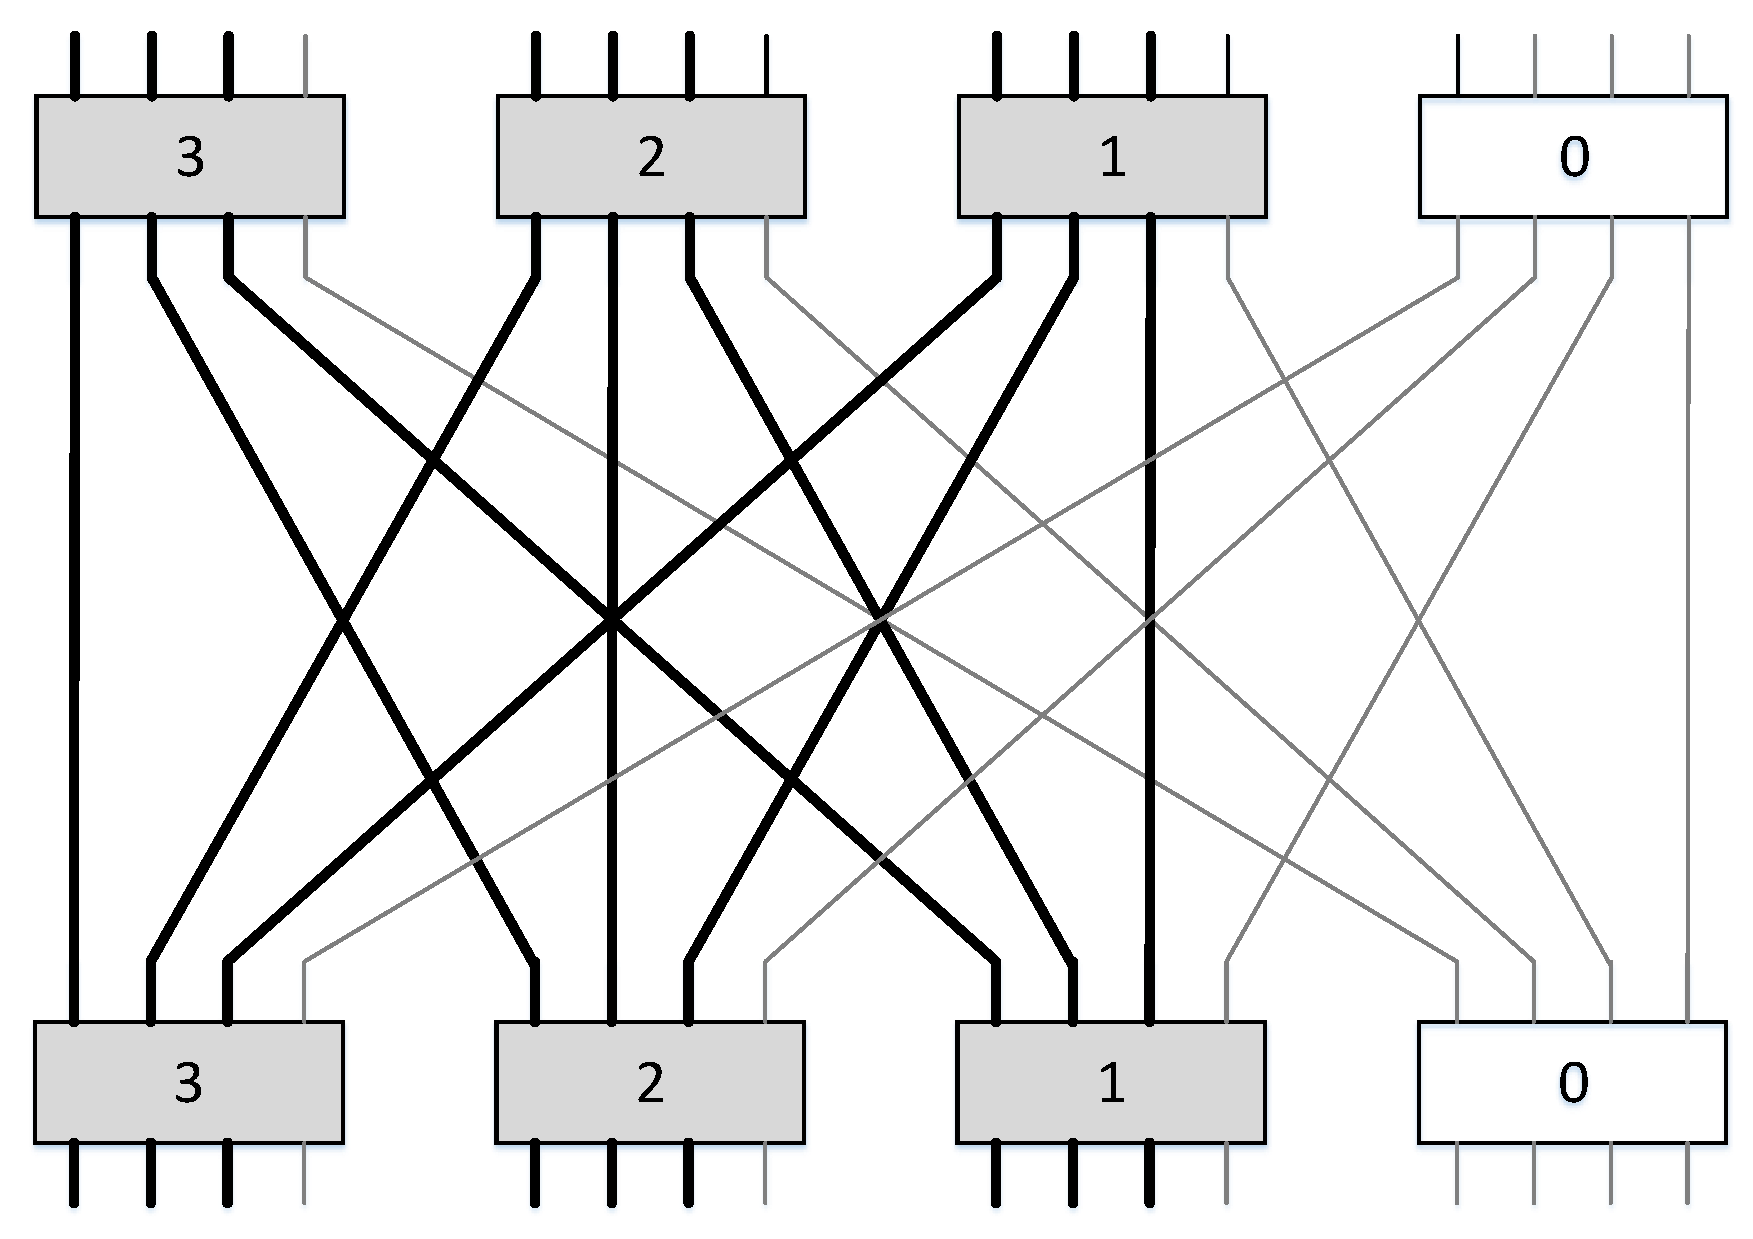
\includegraphics[width=0.9\textwidth,height = 7cm]{images/SMALLPRESENT-4_9bit_trail}
    \caption{9 bit SS trail in SMALLPRESENT-$[4]$.}
    \label{fig:smallpresent_4_player_9bit_trail}
\end{figure}
Fortunately, there is another good trail if we consider the middle two bits of the middle two S-boxes. Because these four bits are involved only among the middle two S-boxes. That is, we have a SS trail of $4$ bits with only $2$ active S-boxes. Figure \ref{fig:smallpresent_4_player_4bit_trail} shows this trail in bold lines. We have used this trail in our experiments later in this chapter.
\begin{figure}[h!]
    \centering
    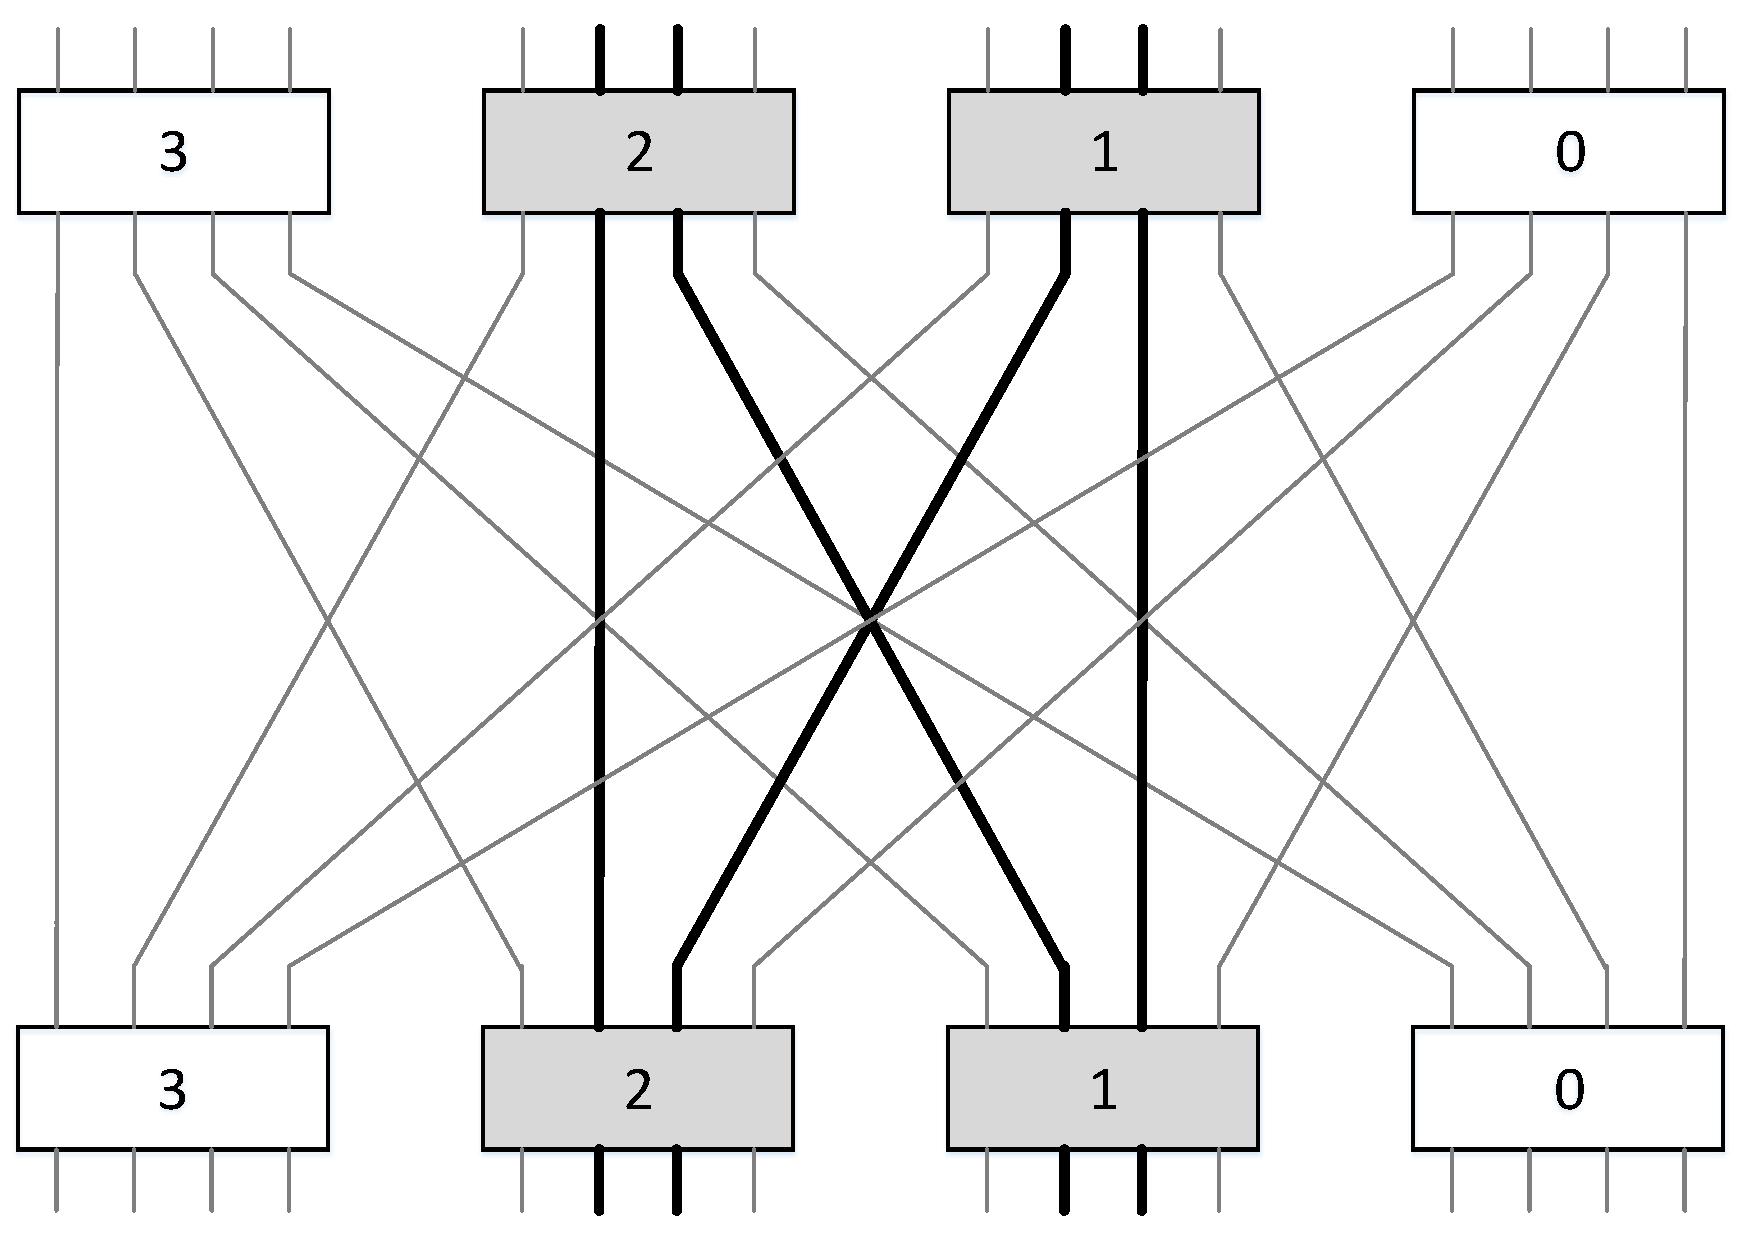
\includegraphics[width=0.9\textwidth,height = 7cm]{images/SMALLPRESENT-4_4bit_trail}
    \caption{4 bit SS trail in SMALLPRESENT-$[4]$.}
    \label{fig:smallpresent_4_player_4bit_trail}
\end{figure}

\subsection{SMALLPRESENT-$[8]$}
In SMALLPRESENT-$[8]$, there are $8$ S-boxes. That means the block size is $32$ bits.   Figure \ref{fig:smallpresent_8_player} shows the non-linear layer of SMALLPRESENT-$[8]$. Based on the principle of choosing an SS trail, we have chosen the trail mentioned in bold lines in this figure. 
\begin{figure}[h!]
    \centering
    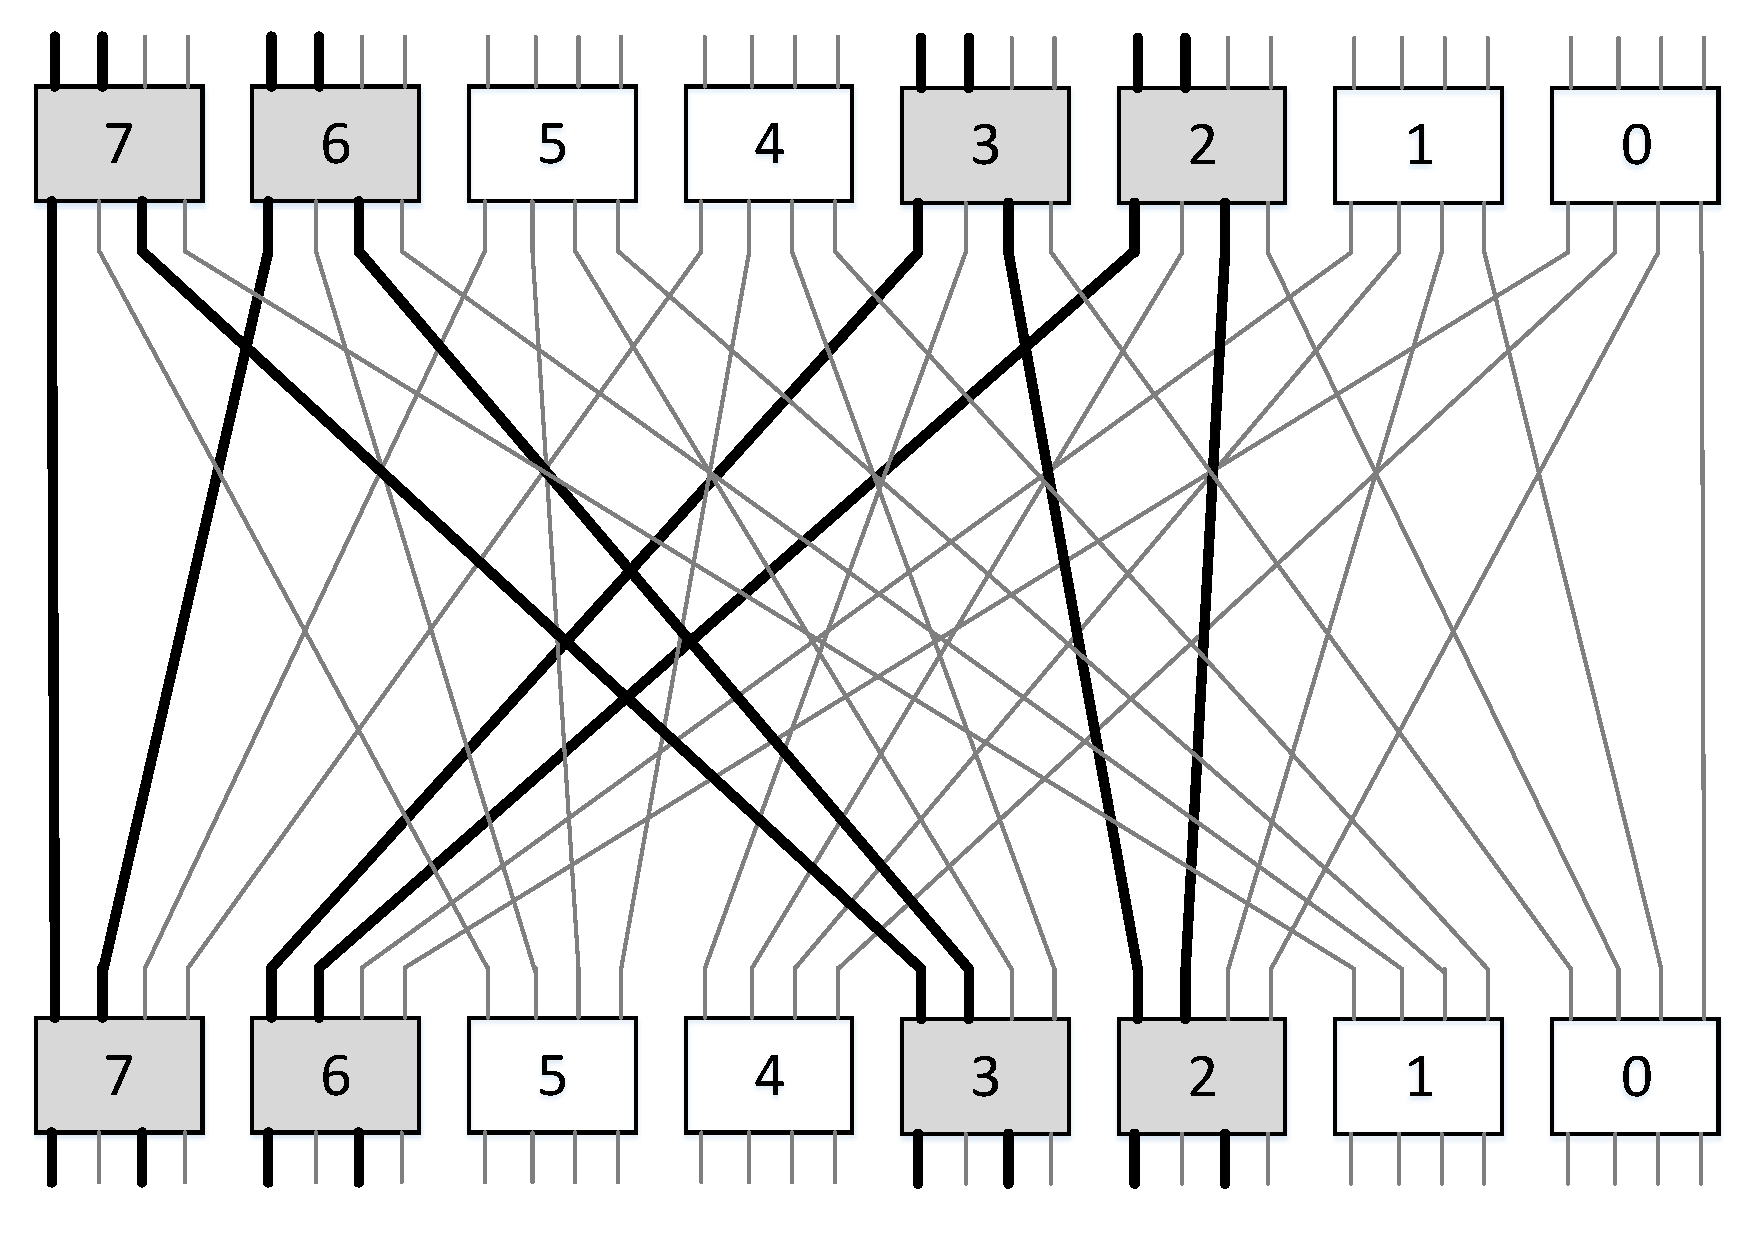
\includegraphics[width=0.9\textwidth,height = 7cm]{images/SMALLPRESENT-8_8bit_trail}
    \caption{8 bit SS trail in SMALLPRESENT-$[8]$.}
    \label{fig:smallpresent_8_player}
\end{figure}
\section{Experiments on SMALLPRESENT-$[4]$}
The trail mentioned in bold lines in Figure \ref{fig:smallpresent_4_player_4bit_trail} is used in these experiments. All the samples that we have used in our experiments are drawn randomly with replacement. At first we investigate the distribution of $C\left(a\right)$ as $a$ varies. As the purpose is to investigate the distribution of $C(a)$, we do not need to consider the key. Then we investigate the distribution of the statistic $T$ for a single fixation where both of the fixation and the sample are varible. Here $a$ is a four bit value, and the size of the distribution is $|Y| = 2^4$.  In the following sections we present the experimental results.
\subsection{SSA Capacities $C(a)$:}
Here $C(a)$ is the capacity of the distribution $p\left(a\right) = \left(p_{\eta}\left(a\right)\right)$ where $a \in \mathbb{F}_2^4$ is the fixation at the input of the trail and $\eta \in \mathbb{F}_2^4$ is the value at the output of the trail. Which means, $C(a)$ is actually $C_{p\left(a\right)}$ as it is defined in Section \ref{section:capacity_of_a_distribution}. And it is computed according to (\ref{eqn:capacity_of_a_distribution}). The experimental value of the variance of $C(a)$ is computed over all the possible fixations $a \in \mathbb{F}_2^4$. The theoretical variance is computed according to Theorem \ref{general capacity distribution}. The result is presented in Table \ref{table:comparing_hypothesis}. \par \noindent From comparative analysis point of view, we observe that, for some numbers of rounds the practical variance is closer to the theoretical one than some other rounds. Now it would be interesting to check how this result agrees with Hypothesis \ref{hyp:hypothesis_on_p_eta_a}. The question is, if the variances of $C(a)$ is  comparatively far from the values predicted by the model, then, is it due to the fact that the probability distributions of $p_{\eta}(a)$ is also far from satisfying the hypothesis? That is, are the variances of  $p_{\eta}(a)$ vary a lot with $\eta$? Similarly, if the variance of $C(a)$ is comparatively closer to the prediction by the model, is it also the case that $p_{\eta}(a)$ have smaller variances? Here $p_{\eta}\left(a\right)$ is calculated using the formula mentioned in (\ref{eqn:p_eta_a}). Which in our case looks like following:
\begin{eqnarray*}
p_{\eta}\left(a\right) = \frac{1}{2^{12}}\left\lbrace x | E_k\left(x,a\right) = \eta  \right\rbrace
\end{eqnarray*}
Table \ref{table:comparing_hypothesis} also compares ``Distance between theoretical and experimental $\sigma^2_{C(a)}$'' with ``variance of $\sigma^2_{p_{\eta}(a)}$ over all $\eta$''
\pagebreak
\begin{center}
\begin{scriptsize}
\captionof{table}{}
\begin{tabular}{l*{4}{c}r} \label{table:comparing_hypothesis}
Round & $C=$ & $\sigma^2_{C(a)}$ &  $\sigma^2_{C(a)}$ & Distance & Variance of $\sigma^2_{p_{\eta}(a)}$ \\
& $\frac{1}{2^4}\sum_{a \in \mathbb{F}_2^4}C(a)$ & (Experimental) & (Theoretical) & & (over all $\eta$)\\
\hline
1 & 1.2500000000 & 0.000000000000 & 0.208333328366 & 0.208333328366 & 0.000000000000000\\
2 & 0.0864257812 & 0.000053644180 & 0.000995922135 & 0.000942277955 & 0.000000000818545\\
3 & 0.0263200998 & 0.000082312916 & 0.000092366354 & 0.000010053438 & 0.000000001487419\\
4 & 0.0084733963 & 0.000012357389 & 0.000009573126 & 0.000002784263 & 0.000000000223686\\
5 & 0.0046606063 & 0.000002714300 & 0.000002896167 & 0.000000181867 & 0.000000000046755\\
6 & 0.0039848089 & 0.000002259238 & 0.000002117160 & 0.000000142078 & 0.000000000014765\\
7 & 0.0029691457 & 0.000000661685 & 0.000001175444 & 0.000000513759 & 0.000000000015007\\
8 & 0.0041698217 & 0.000001235339 & 0.000002318322 & 0.000001082983 & 0.000000000019639\\
9 & 0.0041134357 & 0.000002544029 & 0.000002256047 & 0.000000287982 & 0.000000000015644\\
10 & 0.0029462575 & 0.000001245313 & 0.000001157391 & 0.000000087922 & 0.000000000024034\\
11 & 0.0030920505 & 0.000000583181 & 0.000001274770 & 0.000000691590 & 0.000000000015651\\
12 & 0.0034888982 & 0.000002455807 & 0.000001622988 & 0.000000832819 & 0.000000000030971\\
13 & 0.0038551092 & 0.000001477955 & 0.000001981582 & 0.000000503627 & 0.000000000017599\\
14 & 0.0035421848 & 0.000001178269 & 0.000001672943 & 0.000000494674 & 0.000000000022411\\
15 & 0.0033624172 & 0.000001049226 & 0.000001507447 & 0.000000458220 & 0.000000000015530\\
16 & 0.0040042400 & 0.000001861589 & 0.000002137858 & 0.000000276270 & 0.000000000012828\\
17 & 0.0033563375 & 0.000000747953 & 0.000001502000 & 0.000000754047 & 0.000000000013699\\
18 & 0.0033963918 & 0.000001104406 & 0.000001538064 & 0.000000433658 & 0.000000000016437\\
19 & 0.0035276412 & 0.000001275685 & 0.000001659234 & 0.000000383549 & 0.000000000009210\\
20 & 0.0036349296 & 0.000002631222 & 0.000001761695 & 0.000000869527 & 0.000000000026018\\
21 & 0.0034182071 & 0.000001446692 & 0.000001557885 & 0.000000111193 & 0.000000000017467\\
22 & 0.0035172700 & 0.000004566781 & 0.000001649492 & 0.000002917289 & 0.000000000038211\\
23 & 0.0029666423 & 0.000001265739 & 0.000001173462 & 0.000000092277 & 0.000000000009836\\
24 & 0.0026813745 & 0.000000865261 & 0.000000958636 & 0.000000093375 & 0.000000000012813\\
25 & 0.0035705566 & 0.000002094620 & 0.000001699850 & 0.000000394770 & 0.000000000024349\\
26 & 0.0033077001 & 0.000000503365 & 0.000001458784 & 0.000000955419 & 0.000000000018401\\
27 & 0.0032589435 & 0.000001036276 & 0.000001416095 & 0.000000379819 & 0.000000000020941\\
28 & 0.0035127401 & 0.000002022870 & 0.000001645246 & 0.000000377624 & 0.000000000025578\\
29 & 0.0032626390 & 0.000001063931 & 0.000001419308 & 0.000000355377 & 0.000000000015406\\
30 & 0.0038447380 & 0.000002793566 & 0.000001970935 & 0.000000822632 & 0.000000000035005\\
31 & 0.0032460689 & 0.000001083049 & 0.000001404929 & 0.000000321879 & 0.000000000040317\\
\end{tabular}
\end{scriptsize}
\end{center} \par \noindent Comparatively, we find that the theoretical model disagrees strongly in round $22$ but agrees  better in round $23$. And interestingly we find that the variance of $p_{\eta}(a)$ over all $\eta$ in round $22$ is very large but comparatively small in round $23$. This suggests that the smaller the distance between the theoretical model and  the experimental computation, the closer the hypothesis tends to be valid. %In the next section we will check this phenomenon in the case of statistic $T\left(\phi,a\right)$. 
\par \noindent One important thing to note here is that we do not yet have a proper understanding of what is a small difference or what is a large difference in between the theoretical and experimental values. But we know that our objective is to be a able to distinguish a distribution from random. In other words, we need to know, how useful the theoretical models are, when we use them to perform the statistical test. To visualize this effect, let us check how the theoretical and experimental values of the statistic $T\left(\phi,a\right)$ evolves as the sample size grows and when they start to distinguish from the random distribution.

\subsection{Statistic $T\left(\phi,a\right)$}
\iffalse
Here we will be evaluating Theorem \ref{theorem: variable fixation}. In Table \ref{table:T_a_variable_a_variable_phi_full_codebook}, the comparison is done using sample $\phi$ to be all the possible plaintexts with fixation $a$. So, in the current context $\phi = \mathbb{F}_2^{12}$. The sampling of the chosen plaintexts are done randomly without replacement. 
\begin{center}
\begin{scriptsize}
\captionof{table}{}
\begin{tabular}{l*{4}{c}r} \label{table:T_a_variable_a_variable_phi_full_codebook}
Round & $\mu_{T(\phi,a)}$ &  $\mu_{T(\phi,a)}$ & $\sigma^2_{T(\phi,a)}$ & $\sigma^2_{T(\phi,a)}$ & variance of $\sigma^2_{p_{\eta}(a)}$ \\
 & (Experiment) &  (Theory) & (Experiment) & (Theory) & (over all eta) \\
\hline
1 & 5105.4043 & 5105.4043 & 7138.4285 & 3475353.7379 & 0.000000014823301\\
2 & 372.2495 & 372.2495 & 1908.7264 & 18475.9599 & 0.000000000925185\\
3 & 127.3325 & 127.3325 & 2165.3678 & 2161.8094 & 0.000000002349859\\
4 & 46.7144 & 46.7144 & 314.0983 & 290.9641 & 0.000000000356634\\
5 & 36.2334 & 36.2334 & 171.5494 & 175.0479 & 0.000000000122619\\
6 & 29.6890 & 29.6890 & 66.1217 & 117.5246 & 0.000000000153912\\
7 & 26.7393 & 26.7393 & 142.5548 & 95.3317 & 0.000000000047919\\
8 & 31.2900 & 31.2900 & 128.2649 & 130.5422 & 0.000000000063969\\
9 & 31.0596 & 31.0596 & 147.5356 & 128.6263 & 0.000000000096241\\
10 & 26.8184 & 26.8184 & 37.0340 & 95.8966 & 0.000000000020260\\
11 & 32.7720 & 32.7720 & 71.0487 & 143.2003 & 0.000000000123782\\
12 & 28.8843 & 28.8843 & 82.0928 & 111.2402 & 0.000000000048031\\
13 & 27.8760 & 27.8760 & 82.6281 & 103.6093 & 0.000000000042345\\
14 & 28.1372 & 28.1372 & 84.9019 & 105.5603 & 0.000000000134887\\
15 & 27.6509 & 27.6509 & 101.1446 & 101.9428 & 0.000000000067674\\
16 & 31.7510 & 31.7510 & 102.2708 & 134.4166 & 0.000000000101584\\
17 & 24.4453 & 24.4453 & 111.6897 & 79.6764 & 0.000000000074382\\
18 & 34.2988 & 34.2988 & 150.9873 & 156.8546 & 0.000000000061766\\
19 & 32.1738 & 32.1738 & 139.6693 & 138.0207 & 0.000000000097652\\
20 & 28.4150 & 28.4150 & 93.7672 & 107.6553 & 0.000000000041508\\
21 & 28.3413 & 28.3413 & 96.7962 & 107.0973 & 0.000000000059939\\
22 & 31.7378 & 31.7378 & 106.5411 & 134.3050 & 0.000000000098388\\
23 & 28.8462 & 28.8462 & 136.7566 & 110.9470 & 0.000000000100681\\
24 & 27.6494 & 27.6494 & 61.0345 & 101.9320 & 0.000000000070456\\
25 & 27.4243 & 27.4243 & 153.7815 & 100.2791 & 0.000000000087872\\
26 & 27.3394 & 27.3394 & 60.1927 & 99.6587 & 0.000000000067826\\
27 & 30.8081 & 30.8081 & 83.5536 & 126.5519 & 0.000000000085514\\
28 & 28.8550 & 28.8550 & 165.2511 & 111.0147 & 0.000000000076191\\
29 & 30.2554 & 30.2554 & 197.2302 & 122.0517 & 0.000000000106616\\
30 & 30.2812 & 30.2812 & 223.7799 & 122.2605 & 0.000000000095609\\
31 & 27.1299 & 27.1299 & 76.0133 & 98.1374 & 0.000000000121043\\\end{tabular}
\end{scriptsize}
\end{center}
We observe the same phenomenon here also as we observed in Table \ref{table:comparing_hypothesis}. 
\fi
\par \noindent For each fixation $a$ we draw a line for the statistic $T\left(\phi,a\right)$ computed from experimental data. We plot the size of the sample in the $X$-axis. The same sample is used for all the fixations. That is, For all samples $\phi_1,\phi_2$ used in the experiment, if $|\phi_1| = |\phi_2|$, then $\phi_1 = \phi_2$. And if $|\phi_1| < |\phi_2|$, then $\phi_1 \subset \phi_2$. We also draw the lines for variable fixation and variable sample calculated from theoretical distribution as in Theorem \ref{theorem: variable fixation} and presented in gray color. The dark gray area represents $1$ standard deviation around the theoretical mean. And the light gray area represents $2$ standard deviation around the theoretical mean. We draw the plotting for round $3,4,22$ and $23$ in Figures \ref{fig:T_a_phi_variable_a_varible_phi_variable_size_03rounds}, \ref{fig:T_a_phi_variable_a_varible_phi_variable_size_04rounds},\ref{fig:T_a_phi_variable_a_varible_phi_variable_size_22rounds} and \ref{fig:T_a_phi_variable_a_varible_phi_variable_size_23rounds}. The reason to draw the plot of round $3$ and $4$ is to see how the evolution of the statistic happens in case of smaller number of rounds. And round $22$, $23$ are chosen as they were found interesting in previous section. Observe that, in all the cases of round $3,4,22$ and $23$, they are in close accordance with the theoretical distribution. And in the cases of round $3$ and $4$, both of the theoretical and experimental distribution distinguishes itself from the uniformly random distribution. \par \noindent These plots are also in close accordance with the theoretical data complexity $N_{SS}$ that we have derived in previous chapter. In practice, distinguishing becomes possible when the sample size is large enough so that all the red lines are clearly above the random ($T = 15$). In theory, we can calculate the estimates of $N_{SS}$ using (\ref{eqn:N_ss}). First we set the values of $\zeta_0 = \zeta_1$ to  $\sqrt{2}$ which theoretically suppose to provide $85\%$ success probability of the statistical test. Then using the values of $C$ for the corresponding round gives the theoretical estimation of $N_{SS}$ for that particular round. We see that using this method the theoretical values of $N_{SS}$ for round $3,4,22$ and $23$ are around $2^{10.20},2^{11.84},2^{13.1}$ and $2^{13.35}$ respectively. In contrast, from the experimental plots we see that the red lines start to distinguish at around the same values of $|\phi|$ in the horizontal axis for the case of round $3$ and $4$. From the theoretical values of $N_{SS}$ for round $22$ and $23$, we also find that it distinguishes at the value of $N_{SS}$ which is larger than the full codebook for a fixation. And this is also visible in the plots of those rounds. They do not distinguish at all.

\begin{figure}[h!]
    \centering
    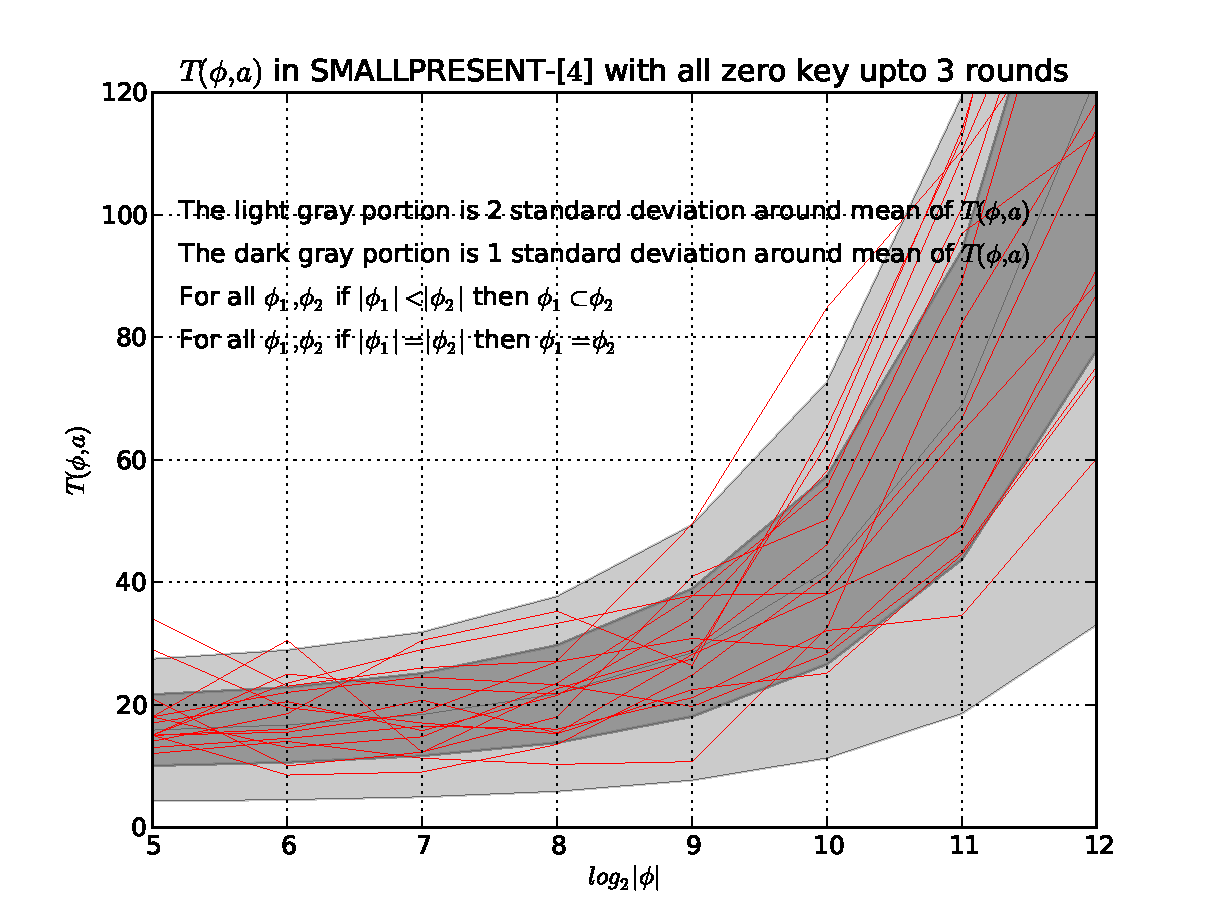
\includegraphics[width=\textwidth , height = 8cm]{images/T_a_phi_variable_a_varible_phi_variable_size_03rounds}
    \caption{$T(\phi,a)$ with $3$ rounds}
    \label{fig:T_a_phi_variable_a_varible_phi_variable_size_03rounds}
\end{figure}

\begin{figure}[h!]
    \centering
    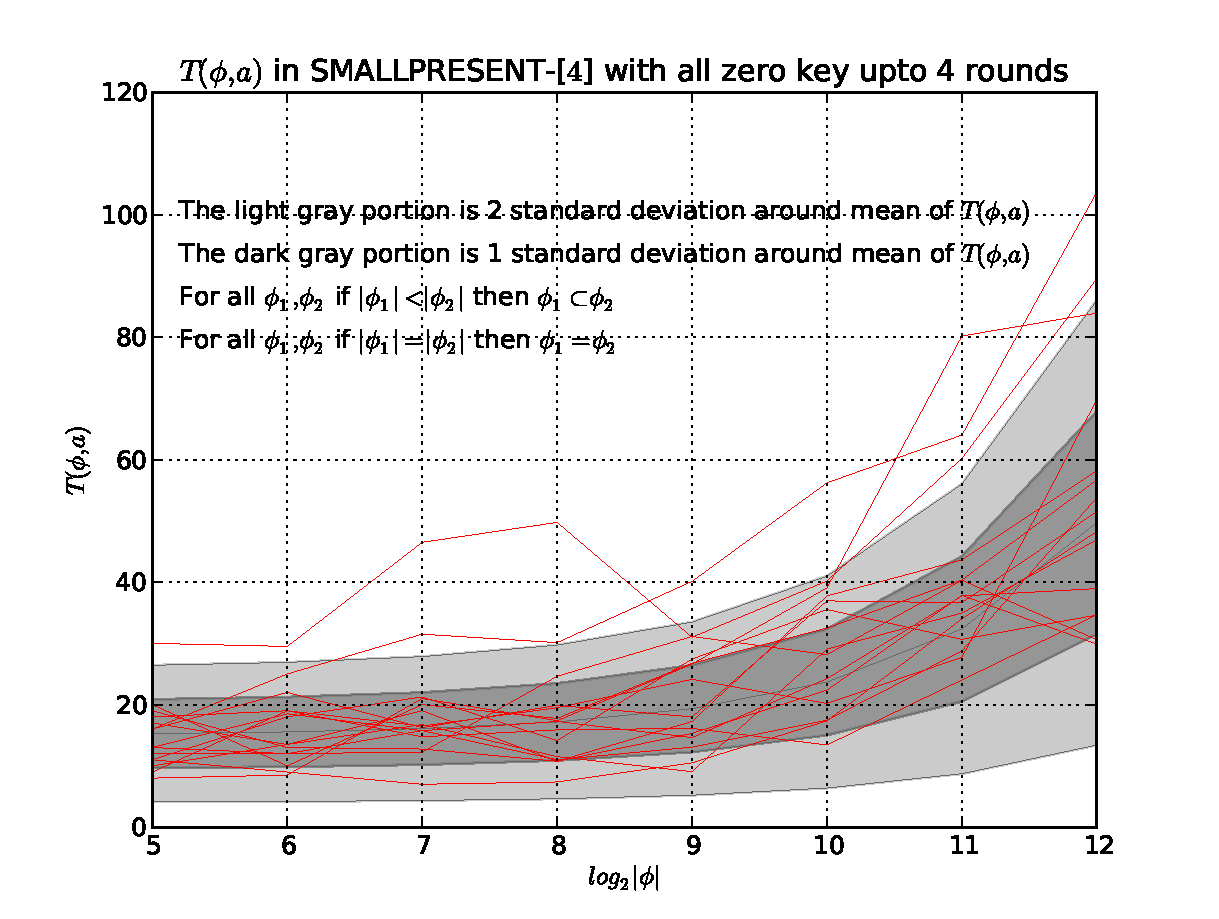
\includegraphics[width=\textwidth , height = 8cm]{images/T_a_phi_variable_a_varible_phi_variable_size_04rounds}
    \caption{$T(\phi,a)$ with $4$ rounds}
    \label{fig:T_a_phi_variable_a_varible_phi_variable_size_04rounds}
\end{figure}

\begin{figure}[h!]
    \centering
    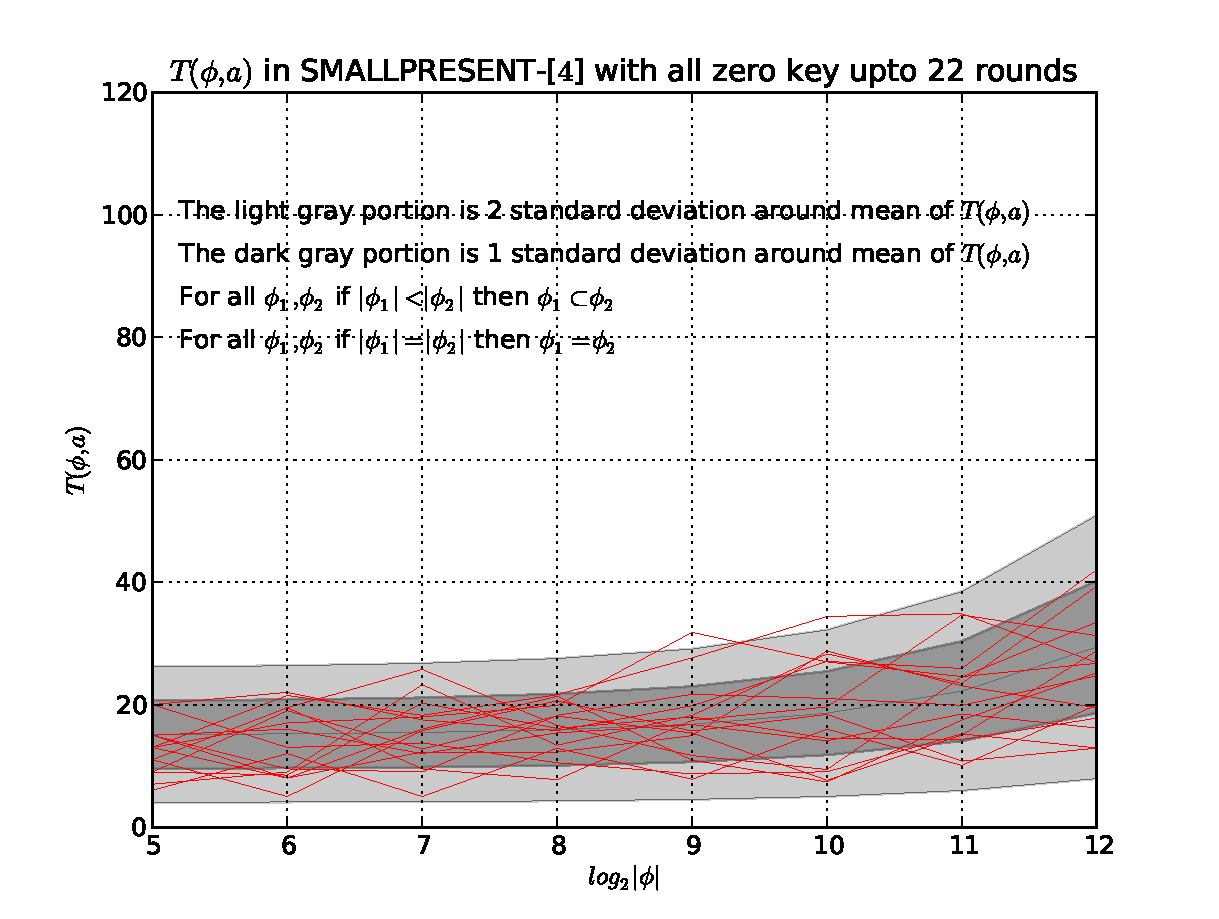
\includegraphics[width=\textwidth , height = 8cm]{images/T_a_phi_variable_a_varible_phi_variable_size_22rounds}
    \caption{$T(\phi,a)$ with $22$ rounds}
    \label{fig:T_a_phi_variable_a_varible_phi_variable_size_22rounds}
\end{figure}

\begin{figure}[h!]
    \centering
    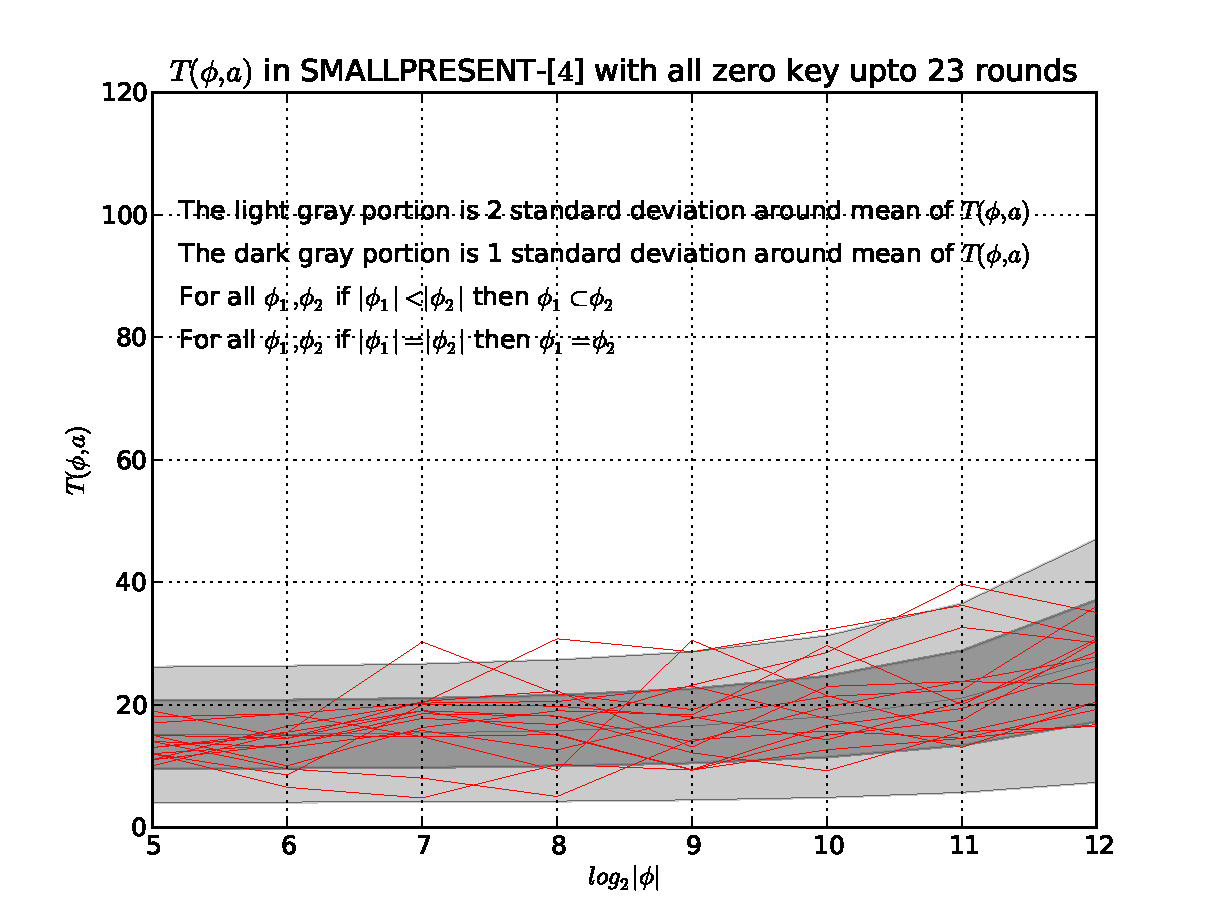
\includegraphics[width=\textwidth , height = 8cm]{images/T_a_phi_variable_a_varible_phi_variable_size_23rounds}
    \caption{$T(\phi,a)$ with $23$ rounds}
    \label{fig:T_a_phi_variable_a_varible_phi_variable_size_23rounds}
\end{figure}%\subsection{Evaluating $T\left(\phi,a\right)$ with $\phi$ sampled randomly with replacement:}
\par \noindent So far, in the experiments of $T\left(\phi,a\right)$, we have used the same sample of equal size for each fixation. Now, let us do the experiment in another way. Let us look at distribution of $T\left(\phi,a\right)$ for a particular round using different fixations and samples of similar sizes. We have used all the possible fixations from 0x0 to 0xf. For each fixation, we have $10000$ samples. Each sample has a size of $2048$ plaintexts and they are chosen randomly with replacement. In this way we had $10000 \times 16 = 160000$ different $T\left(\phi,a\right)$ values. We have calculated the mean and variance of these values of $T$. Then we have compared these with the theoretical values obtained from Theorem \ref{theorem: variable fixation}. Figures \ref{fig:T_a_phi_variable_a_variable_phi_03_round},\ref{fig:T_a_phi_variable_a_variable_phi_04_round},\ref{fig:T_a_phi_variable_a_variable_phi_22_round} and \ref{fig:T_a_phi_variable_a_variable_phi_23_round} shows the theoretical and experimental distribution for round $03,04,22$ and $23$. We observe that the experimental distribution is a little skewed than the theoretical distribution. This is expected as the statistic is originally $\chi^2$ distributed and we have used a normal approximation of $\chi^2$ distribution. As the normal approximation of $\chi^2$ distribution is better satisfied for higher degree of freedom, we understand that the experimental and theoretical distribution will agree better as the number of bits at the output of the SS trail grows. Note that, as like the previous visualization, we observe the same phenomenon in these plots also. For round $3$ it nicely distinguishes from uniform distribution. For round $4$ it looks slightly worse. Nevertheless, it is understandable that the $N_{SS}$ for round $4$ is $2^{11.84}$ and we have used sample of size $2^{11}$ only. And for round $22$ and $23$, they do not distinguishes at all.
\iffalse
\begin{center}
\begin{scriptsize}
\captionof{table}{}
\begin{tabular}{l*{4}{c}r} \label{table:T_a_phi_variable_a_variable_phi}
Round & C & $\mu_{T\left(\phi,a\right)}$ &  $\sigma^2_{T\left(\phi,a\right)}$ & $\mu_{T\left(\phi,a\right)}$ & $\sigma^2_{T\left(\phi,a\right)}$ \\
 & & (Experimental) &  (Experimental) & (Theoretical) & (Theoretical) \\
\hline
15 & 0.003362 & 21.876377 & 61.863674 & 21.885376 & 63.862624355\\
16 & 0.004004 & 23.209412 & 70.374428 & 23.200192 & 71.766521178\\
17 & 0.003356 & 21.855230 & 60.741642 & 21.873088 & 63.790930487
\end{tabular}
\end{scriptsize}
\end{center}
\fi

\begin{figure}[h!]
    \centering
    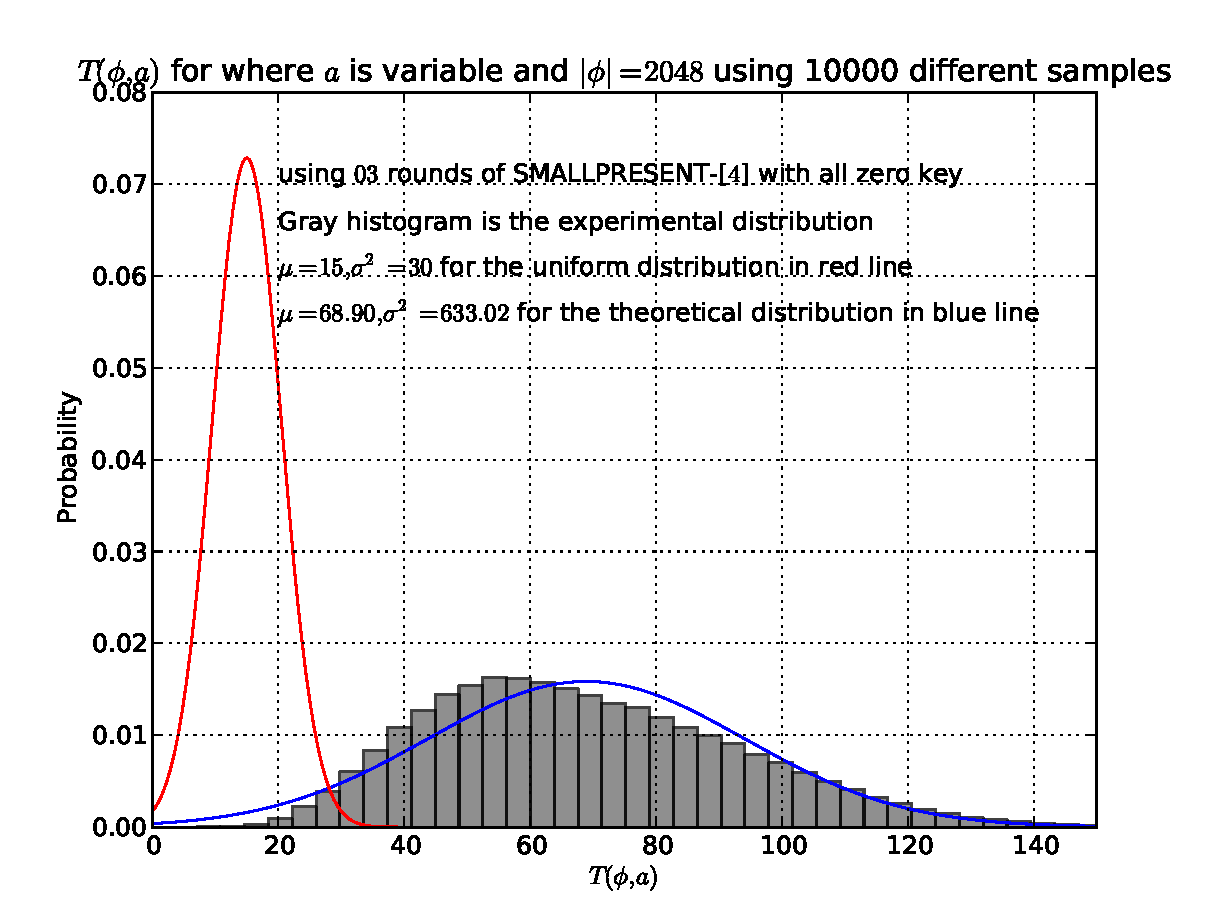
\includegraphics[width= \textwidth , height = 8cm]{images/T_a_phi_variable_a_variable_phi_03_round_plot}
    \caption{$T(\phi,a)$ with $03$ rounds}
    \label{fig:T_a_phi_variable_a_variable_phi_03_round}
\end{figure}
\begin{figure}[h!]
    \centering
    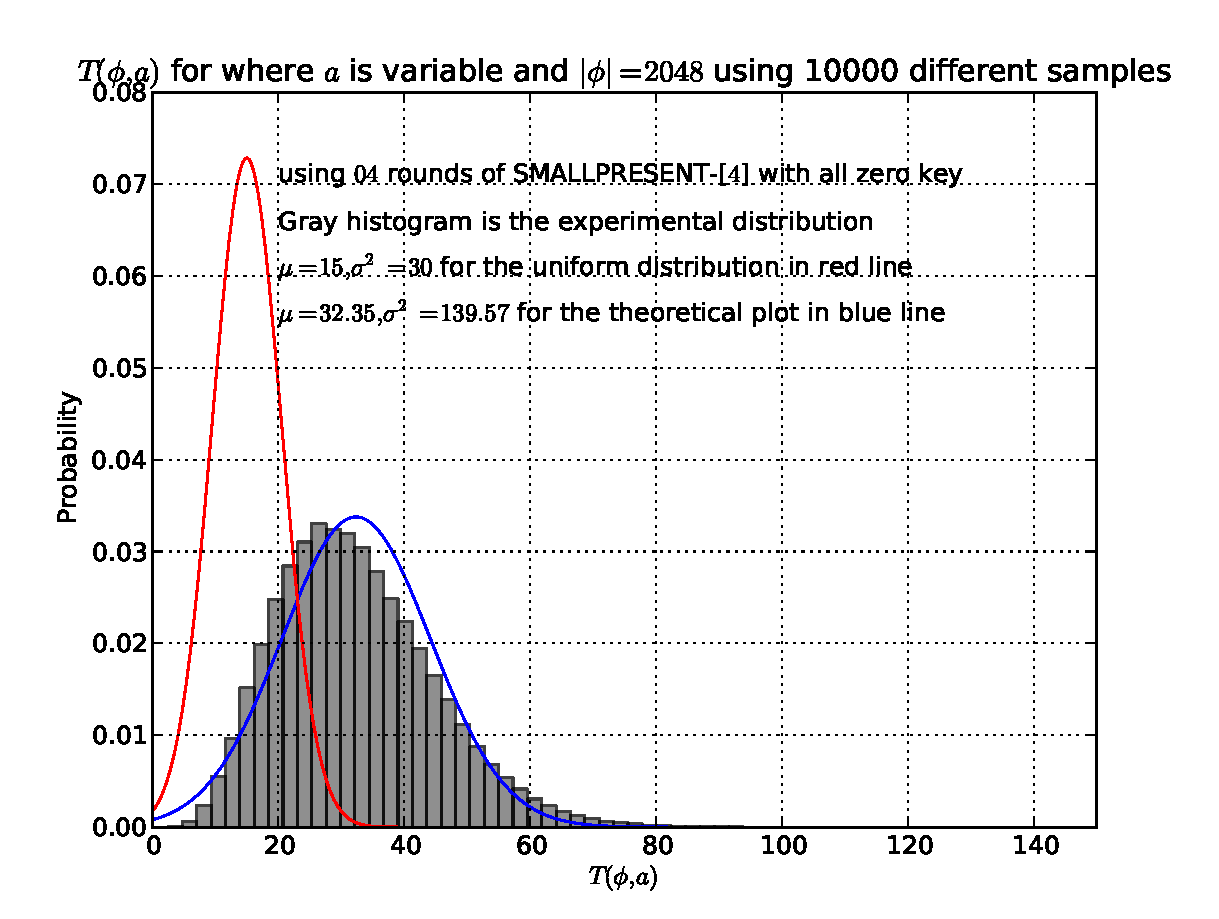
\includegraphics[width=\textwidth , height = 8cm]{images/T_a_phi_variable_a_variable_phi_04_round_plot}
    \caption{$T(\phi,a)$ with $04$ rounds}
    \label{fig:T_a_phi_variable_a_variable_phi_04_round}
\end{figure}

\begin{figure}[h!]
    \centering
    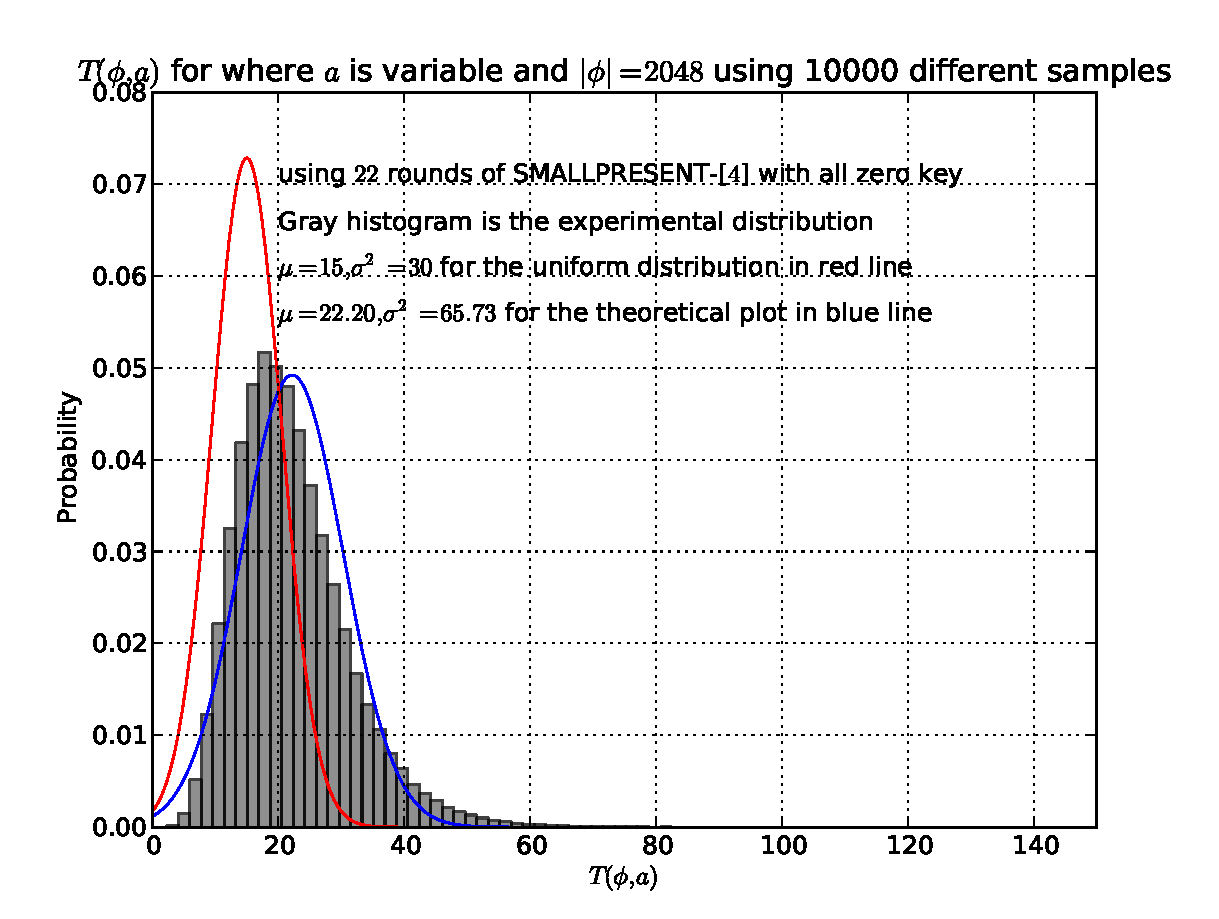
\includegraphics[width=\textwidth , height = 8cm]{images/T_a_phi_variable_a_variable_phi_22_round_plot}
    \caption{$T(\phi,a)$ with $22$ rounds}
    \label{fig:T_a_phi_variable_a_variable_phi_22_round}
\end{figure}

\begin{figure}[h!]
    \centering
    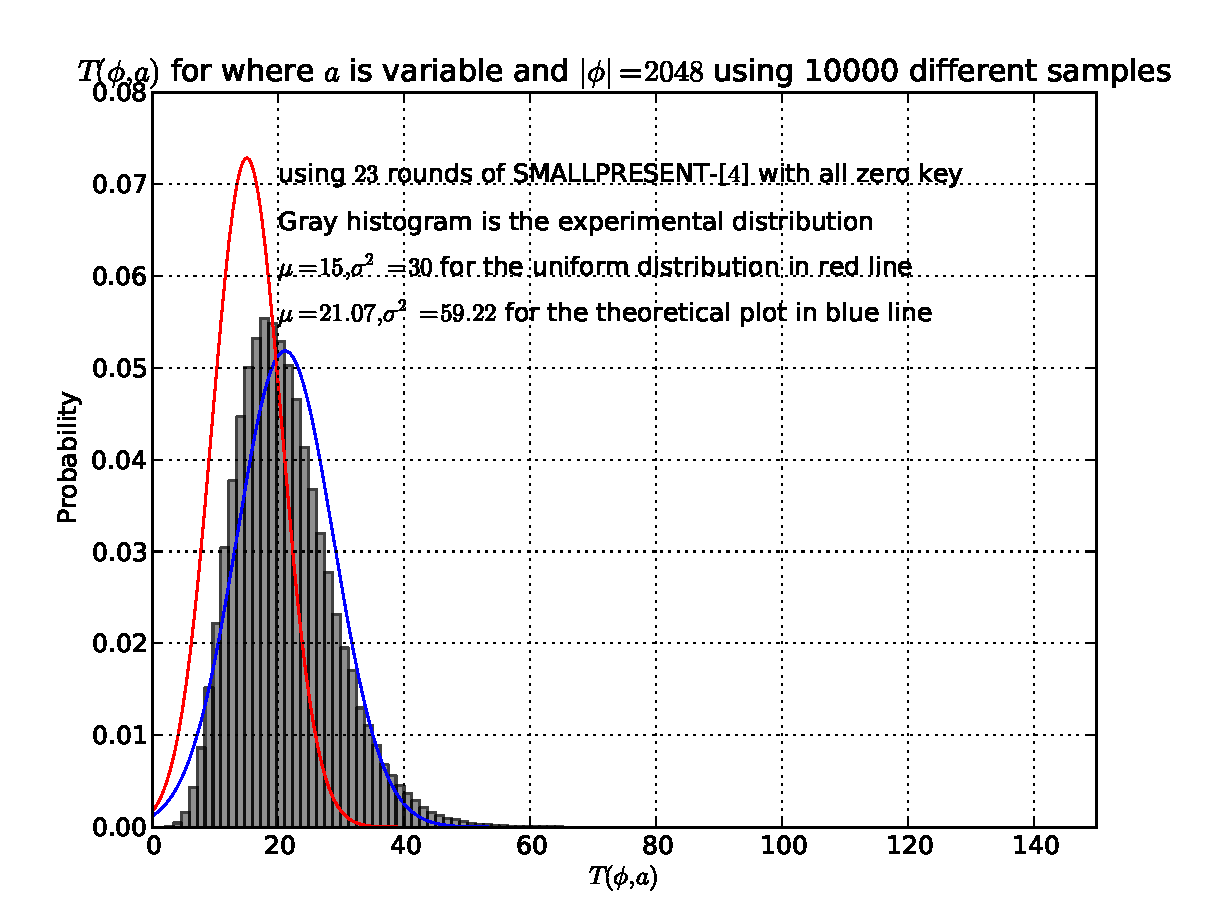
\includegraphics[width=\textwidth , height = 8cm]{images/T_a_phi_variable_a_variable_phi_23_round_plot}
    \caption{$T(\phi,a)$ with $23$ rounds}
    \label{fig:T_a_phi_variable_a_variable_phi_23_round}
\end{figure}

\iffalse

\subsection{Evaluating $T_{a}\left(\phi\right)$ with $\phi$ sampled randomly with replacement:} Here we will be evaluating $T$ for an arbitrarily fixed fixation $a$ or in other words we will now evaluate $T_{a}\left(\phi\right)$ both experimentally and theoretically. We will generate a set $\Phi$ of size $10000$ where each $\phi \in \Phi$ is a randomly chosen (with replacement) subset of  $\mathbb{F}_2^{12}$ and $|\phi| = 2048$. Now for each $\phi \in \Phi$ we will calculate $T_{a}\left(\phi\right)$ according to (\ref{eqn:T_fixed_a_variable_phi}). After that we will calculate the mean and variance of $T_{a}\left(\phi\right)$ over all these $10000$ different $\phi \in \Phi$. And compare this experimentally calculated mean and variance with the theoretically computed mean and variance mentioned in (\ref{eqn:distribution_of_T_fixed_a_variable_phi}). The evaluation is done for $15$ rounds of SMALLPRESENT-$[4]$ and the result is mentioned in Table \ref{table:T_a_phi_fixed_a_variable_fixation}


\begin{center}
\begin{scriptsize}
\captionof{table}{};
\begin{tabular}{l*{4}{c}r} \label{table:T_a_phi_fixed_a_variable_fixation}
$a$ & $\mu_{T_{a}(\phi)}=$ &  $\sigma^2_{T_{a}(\phi)}$ & $C\left(a\right)$ & $\mu_{T_{a}(\phi)}$ & $\sigma^2_{T_{a}(\phi)}$ \\
 & (Experimental) &  (Experimental) &  & (Theoretical) & (Theoretical) \\
\hline
0 & 23.157768 & 64.339134 & 0.004002 & 23.196096 & 62.784384\\
1 & 18.906876 & 45.224827 & 0.001917 & 18.926016 & 45.704064\\
2 & 23.397097 & 63.523018 & 0.004129 & 23.456192 & 63.824768\\
3 & 21.665363 & 56.201130 & 0.003254 & 21.664192 & 57.475968\\
4 & 23.054449 & 61.329144 & 0.003965 & 23.12032 & 62.48128\\
5 & 19.875065 & 49.953552 & 0.002335 & 19.78208 & 49.12832\\
6 & 21.375246 & 55.578331 & 0.003141 & 21.432768 & 55.731072\\
7 & 22.893190 & 60.276630 & 0.003887 & 22.960576 & 61.842304\\
8 & 22.650137 & 62.154163 & 0.003790 & 22.76192 & 61.04768\\
9 & 24.233036 & 63.354294 & 0.004581 & 24.381888 & 67.527552\\
a & 21.359844 & 54.811600 & 0.003134 & 21.418432 & 55.673728\\
b & 17.972765 & 41.687294 & 0.001431 & 17.930688 & 41.722752\\
c & 26.178656 & 74.850182 & 0.005449 & 26.159552 & 74.638208\\
d & 22.964476 & 60.390213 & 0.003950 & 23.0896 & 62.3584\\
e & 19.844593 & 50.031105 & 0.002382 & 19.878336 & 49.513344\\
f & 19.990053 & 50.301014 & 0.002451 & 20.019648 & 50.078592\\
\end{tabular}
\end{scriptsize}
\end{center} \par \noindent Figure \ref{fig:T_a_phi_with_15_rounds_0x00},\ref{fig:T_a_phi_with_15_rounds_0x07}, \ref{fig:T_a_phi_with_15_rounds_0x0b}  shows the distribution of $T_a(\phi)$ for different fixations
\begin{figure}[h!] 
    \centering
    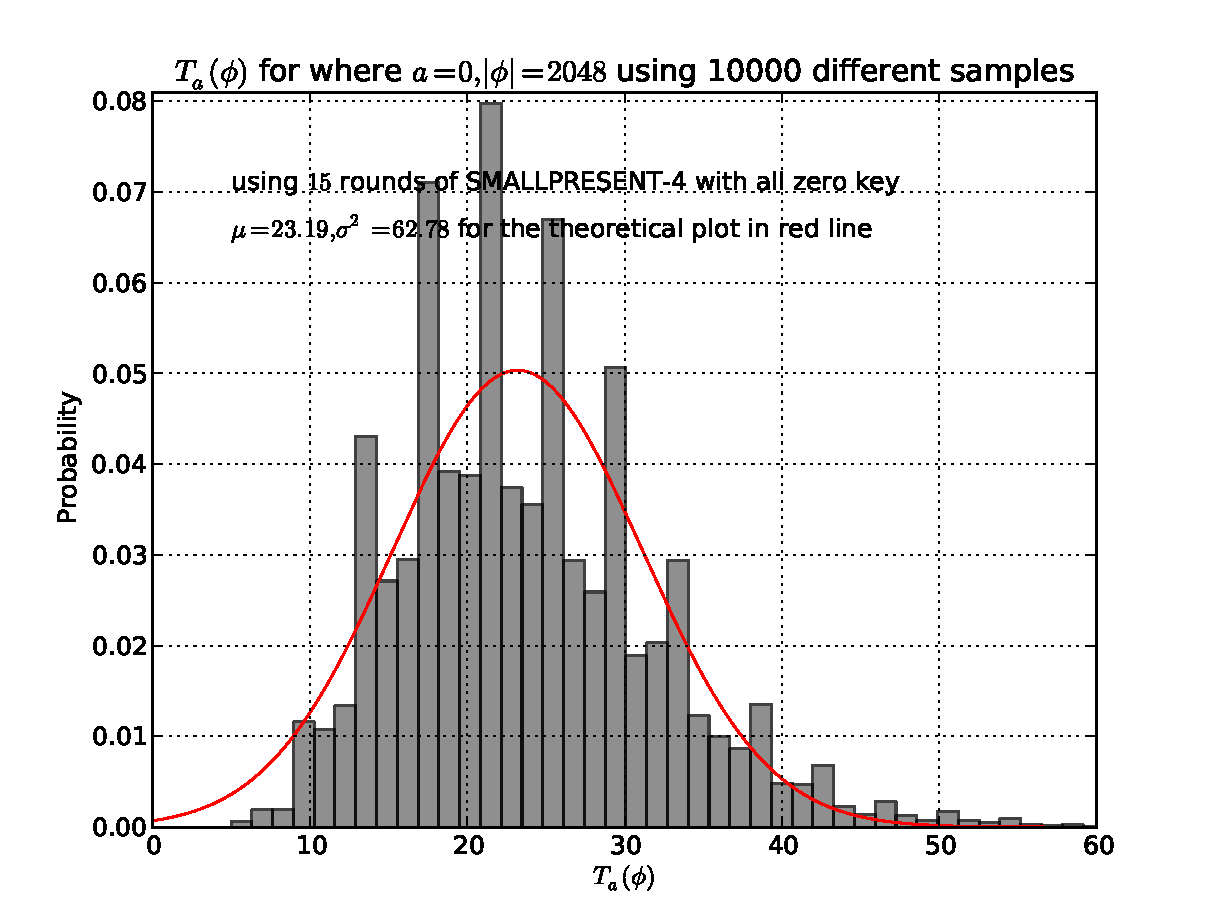
\includegraphics[width=\textwidth , height = 8cm]{images/T_fixed_a_with_value_0_and_variable_phi_size_2048_with_10000_samples}
    \caption{$T_a(\phi)$ with $15$ rounds}
    \label{fig:T_a_phi_with_15_rounds_0x00}
\end{figure}
\begin{figure}[h!]
    \centering
    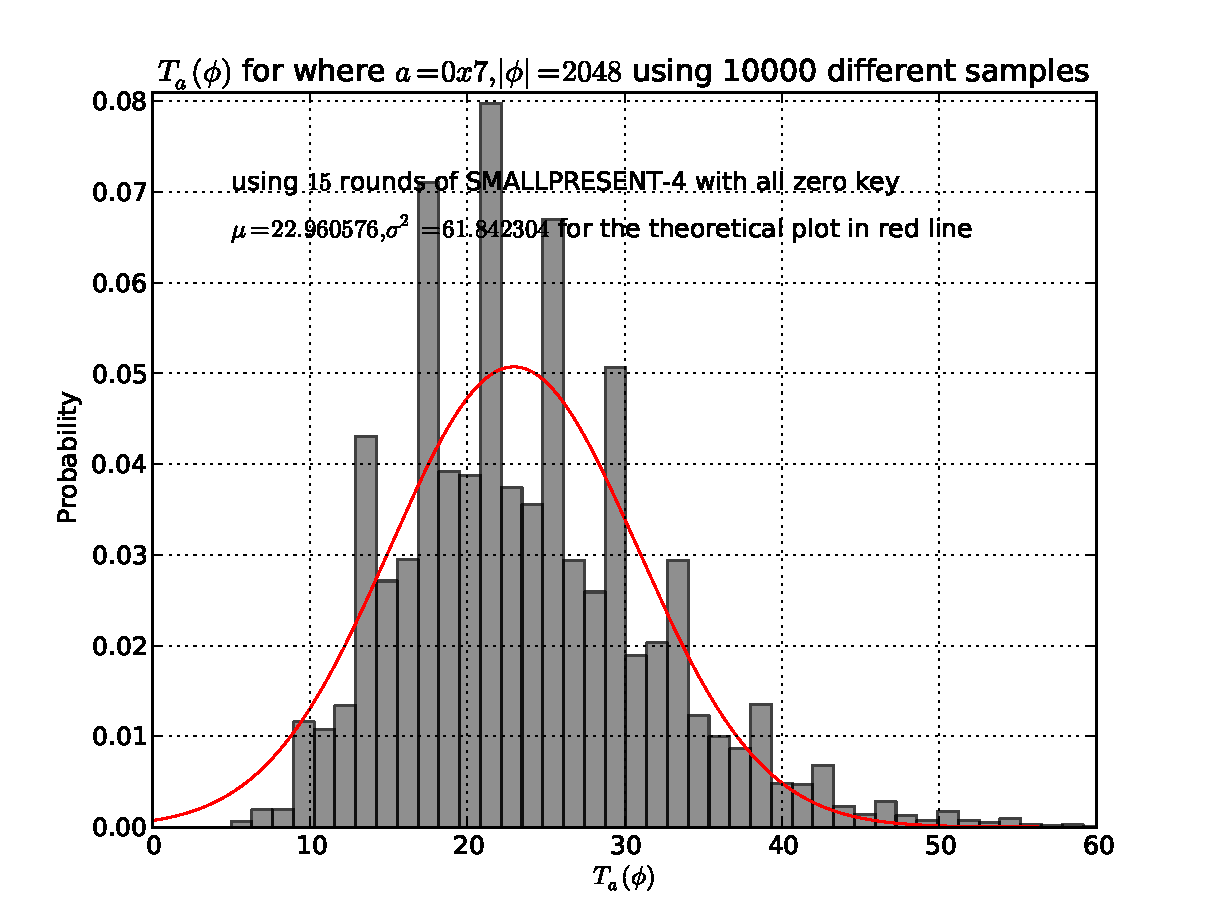
\includegraphics[width=\textwidth , height = 8cm]{images/T_fixed_a_with_value_0x7_and_variable_phi_size_2048_with_10000_samples}
    \caption{$T_a(\phi)$ with $15$ rounds}
    \label{fig:T_a_phi_with_15_rounds_0x07}
\end{figure}
\begin{figure}[h!]
    \centering
    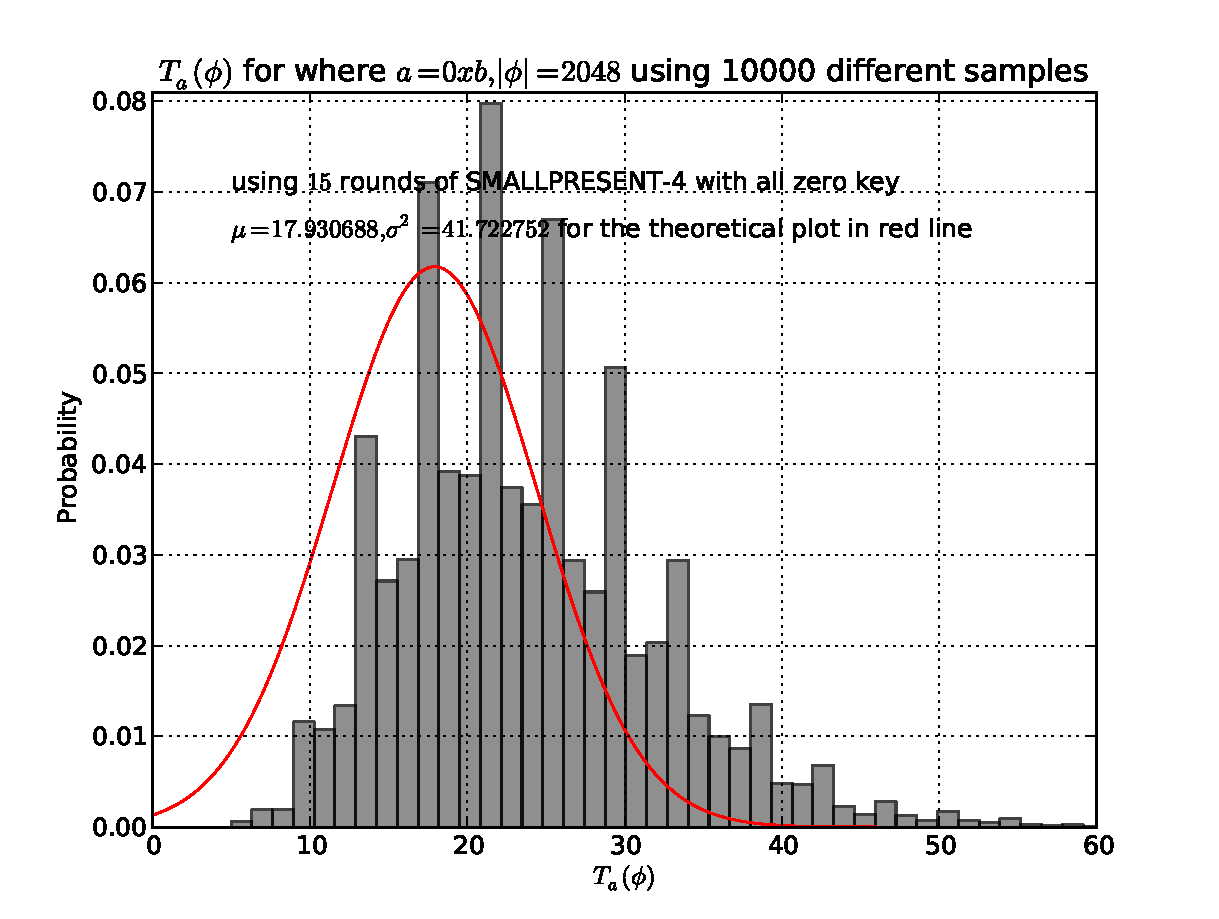
\includegraphics[width=\textwidth , height = 8cm]{images/T_fixed_a_with_value_0xb_and_variable_phi_size_2048_with_10000_samples}
    \caption{$T_a(\phi)$ with $15$ rounds}
    \label{fig:T_a_phi_with_15_rounds_0x0b}
\end{figure} \par \noindent
We observe that there are some spikes in case of a single fixed fixation. But in case variable fixation the theoretical and experimental distribution agrees better.
\fi 
 
\chapter{Conclusions}
\label{chapter:conclusions}
SSA is a comparatively recent statistical cryptanalytic technique among various others, as for example linear and differential cryptanalysis. Researchers have tried and established statistical links among different techniques. Blondeau and Nyberg showed one important link in between TD and SS attacks. They showed that TD attack using structures is identical to the sampling algorithm of SSA \citep{Celine_Kaisa_Links_2014}. Then they used the statistical model of the TD attack to explain the behaviour of SS attack. However, there was no statistical model available which was developed based on the properties of SSA directly. In this thesis, we used the distribution at the output of an SS trail directly to develop a statistical model instead of using any link with other techniques. \par \noindent If an SS trail is chosen wisely as discussed in Chapter \ref{chapter:block_cipher_cryptanalysis}, then there is a significant degree of non-uniformity in the distribution of the values at the output of the trail. %In this thesis we have discussed the principle of choosing a useful SS trail which has significant non-uniformity at the output of the trail. 
As discussed in Chapter \ref{chapter:block_cipher_cryptanalysis}, to perform an SSA, we are in need of an attack that distinguishes the non-uniform distribution from uniform distribution, which eventually can be transformed into a key recovery attack. This thesis has focused only on this distinguishing attack and has not discussed the key recovery attack in detail. In Chapter \ref{chapter:statistics}, we have presented a statistical test that can perform this distinguishing attack. To perform the statistical test %we were in need of a known non-uniform distribution. So, we continued to 
we have developed the statistic $T$ based on the distribution of the values at the output bits of the SS trail, when the bits at the input of the SS trail are fixed and sufficiently many plaintexts are encrypted. The plaintexts differ from each other only in the non-trail input bits. \par \noindent In Chapter \ref{chapter:statistical_distinguishers}, we have derived the distribution of a few different variants of this statistic $T$. We have shown that all of these variants of $T$, which are originally $\chi^2$ distributed are also approximately normally distributed. The mean and variance of all of these variants of $T$ are also derived in this chapter, which enables us to perform the statistical test. We also have derived a reasonable overestimation of the number of required plaintexts (in Chapter \ref{chapter:data_complexity_of_SSA}) to be encrypted to perform the distinguishing attack with an arbitrarily fixed success probability, which is referred as the data complexity of SSA and denoted by $N_{SS}$. Finally, in Chapter \ref{chapter:experiment}, we have verified the statistical model by experimenting on a small variant of the block cipher PRESENT called SMALLPRESENT-[$4$] for the case of a single fixation. The result shows that, the distinguishing attack is successful with very high success probability within the theoretical data complexity bound for smaller rounds. For large number of rounds, the theoretical data complexity is larger than the full code book excluding the fixed bits. As a result they do not distinguish at all using a single fixation. It could be the case that if we used multiple fixations, the distinguisher would distinguish itself from the uniform distribution. That is, there is a scope of more experiments based on multiple fixations.
\par \noindent Both in the theories and experiments it has been considered that, the sample for each fixation is chosen randomly with replacement. When the sample size approaches the full code book excluding the fixed bits, the only sensible option is to use sampling without replacement. However, in real life cryptanalysis the sample size almost never appraoches the full codebook. As a result, we recon, sampling with replacement is good enough for a successfull distinguishing attack. However, in an upcoming paper \citep{kaisa_mohsin_2015},  the case of sampling without replacement is considered. And the experiments have also been extended to SMALLPRESENT-[$8$] for both of the cases of sampling with or without replacement.

%%%%%%%%%%%%%%%%%%%%%%%%%%%%%%%%%%%%%%%%%%%%%%%%%%%%%%%%%%%%%%%%%%%%%%%%%%%%%%%%%%%%%%%%%%%%%%%%%%%%%%%%%%%%%%%%%%%%%%%%%%%%%%
%%%%%%%%%%%%%%%%%%%%%%%%%%%%%%%%%%%%%%%%%%%%%%%%
\iffalse
\par that we used to perform the statistical test. We fixed the bits at the input of the SS trail and encrypted sufficiently many plaintexts which differed from each other only in the non-trail input bits. Then we observed the distribution of the values at the output bits of the trail. We computed a statistic from this distribution which is originally $\chi^2$ distributed. Then we showed that this statistic is approximately a normal deviate and can be used to perform the distinguishing attack. We computed the distribution of a few different variants of this statistic. We also computed a reasonable overestimation of the number of required plaintexts to be encrypted to perform the distinguishing attack with a certain high success probability, which we called to be the data complexity of the attack. We validated this statistical model by experimenting on a small variant of the block cipher PRESENT called SMALLPRESENT-[$4$]. We found that, the distinguishing attack was successful with almost probability $1$ within the theoretical data complexity bound for smaller rounds. We kept our experiment limited for the case of single fixations. For higher rounds, the theoretical data complexity was larger than the full code book excluding the fixed bits. So, it could be the case that if we use multiple fixations, the distinguisher will distinguish itself from the uniform distribution. That is, there is a scope of more experiments based on multiple fixations. \par \noindent Both in our theory and experiment we considered that, the sample for each fixation was chosen randomly with replacement. However, as a future work, it will be very interesting to check how the theory evolves when the sampling is done without replacement. And the experiment could also be extended to SMALLPRESENT-[$8$] for both of the cases of sampling with or without replacement.
\fi

% Load the bibliographic references
% ------------------------------------------------------------------
% You can use several .bib files:
% \bibliography{thesis_sources,ietf_sources}
\bibliography{sources}{}
\bibliographystyle{plain}

% Appendices go here
% ------------------------------------------------------------------
% If you do not have appendices, comment out the following lines
\appendix
%\chapter{First appendix}
\label{chapter:first-appendix}

This is the first appendix. You could put some test images or verbose data in an
appendix, if there is too much data to fit in the actual text nicely.

For now, the Aalto logo variants are shown in Figure~\ref{fig:aaltologo}.

\begin{figure}
\begin{center}
\subfigure[In English]{
\includegraphics[width=.8\textwidth]{images/aalto-logo-en}}
\subfigure[Suomeksi]{
\includegraphics[width=.8\textwidth]{images/aalto-logo-fi}}
\subfigure[P� svenska]{
\includegraphics[width=.8\textwidth]{images/aalto-logo-se}}
\caption{Aalto logo variants}
\label{fig:aaltologo}
\end{center}
\end{figure}


% End of document!
% ------------------------------------------------------------------
% The LastPage package automatically places a label on the last page.
% That works better than placing a label here manually, because the
% label might not go to the actual last page, if LaTeX needs to place
% floats (that is, figures, tables, and such) to the end of the 
% document.
\end{document}
